%\documentclass[11pt,a4paper]{article}
\documentclass[11pt,a4paper]{scrartcl}
%\documentclass[11pt,a4paper,oneside]{book}
\usepackage[british,UKenglish,USenglish,english,american]{babel}
%\usepackage[a4paper, total={16cm, 23cm}]{geometry}
\usepackage[tmargin = 1.25in,bmargin = 1.25in,lmargin = 0.75in,rmargin = 0.75in]{geometry}
\usepackage{tikz}
\usepackage{graphicx}
\usepackage{pgfplots}
\pgfplotsset{width=12cm,compat=1.9}
\usepackage{setspace}
\usepackage{chemmacros}
\usepackage{chemfig}
%\usepackage{ghsystem}
%\usechemmodule{redox}
%\usepackage{chemnum}
%\usepackage{bohr}
%\usepackage{elements}
%\usepackage{endiagram}
%\usepackage{modiagram}
%\usepackage{chemgreek}
%\usepackage{mhchem}
\usepackage{esint}
\usepackage{tabularray}

\usepackage{makeidx}
\usepackage{epstopdf}

\usepackage{amssymb}
\usepackage{mathrsfs}
%\usepackage{minted}
\usepackage{bm}
\usepackage{amsmath}
\usepackage{enumitem}
\usepackage[english]{varioref}
\usepackage[english]{babel}
\usepackage{lipsum}
\usepackage{fancyhdr}
\pagestyle{fancy} 
\usepackage{float}
\usepackage{empheq}
\usepackage[framemethod=tikz]{mdframed}
\usepackage{epstopdf}
\numberwithin{equation}{section}
\usepackage{eso-pic}
\usepackage{calc}
\usepackage{nccmath}
\usepackage{caption}
\usepackage{subcaption}
\usepackage{gensymb}
\usepackage{amsfonts,amsthm,epsfig,epstopdf,titling,url,array}
\usepackage{siunitx}
\sisetup{input-digits = 0123456789\pi}
\usepackage[symbol]{footmisc}
\usepackage{xcolor}
\usepackage{multicol}
\usepackage{boondox-cal}
\DeclareSIUnit\atm{atm}
\setcounter{secnumdepth}{3}
\setcounter{tocdepth}{3}
\usepackage{booktabs}
\usepackage{blindtext}
\usepackage{changepage}
\usepackage{longtable}

% \usepackage{draftwatermark}
% \SetWatermarkText{DRAFT}
% \SetWatermarkScale{5}

\DeclareSIUnit\atm{atm}

\pagestyle{fancy} 
\fancypagestyle{firstpage}{
	\rhead{
	}
}
\fancyhead[L]{\small\slshape\nouppercase{\leftmark}}
\chead{}
\rhead{
}
\lfoot{\textit{}}
\cfoot{-\ \thepage\ -}
\rfoot{\textit{}}

\DeclareMathOperator{\rank}{rank}
\DeclareMathOperator{\atantwo}{atan2}
\DeclareMathOperator{\arctantwo}{arctan2}
\DeclareMathOperator{\spn}{span}

\renewcommand{\headrulewidth}{0.4pt}
\renewcommand{\footrulewidth}{0.4pt}
\newcommand{\abs}[1]{\left|#1\right|}
\definecolor{mycolor1}{rgb}{0.97, 0.97, 0.97}
\definecolor{mycolor2}{rgb}{0.97, 0.97, 0.97}
\definecolor{tableShade}{gray}{0.9}
\newcommand{\sign}{\text{sign}}
\newcommand{\centered}[1]{\begin{tabular}{@{}l@{}} #1 \end{tabular}}
\theoremstyle{it}
\newtheorem{defn}{Definition}[section]
\newtheorem{assumption}{Assumption}[section]
\newtheorem{thm}{Theorem}[section]
\newtheorem{lemma}{Lemma}[section]
\newtheorem{corollary}{Corollary}[section]
\theoremstyle{definition}
%\theoremstyle{it}
\newtheorem{example}{Example}[section]
\let\eqrefn\eqref
\renewcommand{\eqref}[1]{Eq.~(\ref{#1})}

\newenvironment{myitemize_1}
{ \begin{itemize}[topsep=4pt]
		\setlength{\topsep}{2pt}		
		\setlength{\itemsep}{2pt}
		\setlength{\parskip}{2pt}
		\setlength{\parsep}{2pt}    }
{ \end{itemize}                  	}

\newenvironment{myitemize_2}
{ \begin{itemize}[topsep=4pt]
		\setlength{\topsep}{2pt}		
		\setlength{\itemsep}{2pt}
		\setlength{\parskip}{2pt}
		\setlength{\parsep}{2pt}    }
{ \end{itemize}   					}


\newmdenv[innerlinewidth=0.5pt, roundcorner=4pt,backgroundcolor=mycolor2, 
linecolor=mycolor1,innerleftmargin=6pt,
innerrightmargin=6pt,innertopmargin=6pt,innerbottommargin=6pt]{mybox}

\title{\textbf{ 
		\begin{LARGE}
			Modularity:
		\end{LARGE} \\[24pt]
		\begin{Large}
			model and control architecture
	\end{Large}}
}
\author{\textbf{Davide Bagnara}}

\begin{document}
	\thispagestyle{empty}
	\begin{mybox}
		\maketitle
		\vspace{100mm}
	\end{mybox}
	%	\let\clearpage\relax
	\newpage
	\tableofcontents%
	\listoffigures%
	\listoftables
	%	\let\clearpage\LaTeXStandardClearpage
	\newpage
	
\begin{onehalfspace}
\section{Introduction}	
To introduce the work described along the document, it could be useful to start from a generic configuration which the \textit{ElectricalDrive} are subjected, as shown in Figure~\ref{ElectricalDrive_connection_figure_1b}.
\begin{figure}[H]
	\centering
	\includegraphics[width = 450pt, angle = 0, 
	keepaspectratio]{figures/ElectricalDrive_connection.eps}
	\captionsetup{width=0.75\textwidth, font=small}	
	\caption{Functional representation of the electrical drives (\textit{ElectricalDrive}) configuration respect to the PSM modularity and the grid connection. Each, galvanically isolated three phase system of the PSM has been connected to a specific electrical drive.}
	\label{ElectricalDrive_connection}
\end{figure}
Figure~\ref{ElectricalDrive_connection} shows a typical configuration where each independent, and galvanically isolated, PSM (permanent magnet synchronous machine/generator) three phase system is connected to a corresponding \textit{ElectricalDrive}, or in other words each independent three phase system, available in the PSM, is connected to a \textit{ElectricalDrive} to achieve the system requirements in terms of torque and power. \\

Each \textit{ElectricalDrive} is basically made by an AFE (active front end) and an INVERTER (driver of the PSM), and while the INVERTER is connected to a independent PSM three phase system, AFE is connected to the the grid, by a proper grid filter and electromechanical protections\footnote{This document will not focus on electromechanical equipment, but mainly on the effect of parallelization on resulting residual harmonic spectrum of the grid current}.\\

\noindent\textbf{Remark} - by the use of additional control strategies the \textit{ElectricalDrive} can be connected in hard-parallelization\footnote{In this document hard-parallelization means the at least two \textit{ElectricalDrive} are connected together either at AFE side as well as at INVERTER side.} i order to form a single thee phase electrical PSM system, as shown in Figure~\ref{ElectricalDrive_connection_hp}\footnote{The \textit{ElectricalDrive} used for hard-parallelization is equipped with additional common mode inductance, the PWM modulator of each switching stage (AFEn as well as INVERTERn) is synchronized respect to a master timing, moreover, an additional zero sequence current loop control is activated.}. 

\begin{figure}[H]
	\centering
	\includegraphics[width = 450pt, angle = 0, 
	keepaspectratio]{figures/ElectricalDrive_connection_hp.eps}
	\captionsetup{width=0.75\textwidth, font=small}	
	\caption{Functional representation of the electrical drives (here ElectricalDrive) configuration respect to the PSM modularity and the grid connection. The INVERTER output stage of each \textit{ElectricalDrive} has been connected among each other to create a single three phase system. The ElectricalDrive used for this special configuration are equipped with common mode inductors and PWM synchronization mechanism as well as a common mode current loop.}
	\label{ElectricalDrive_connection_hp}
\end{figure}

In general when an installation has a nominal power major than 250kW a medium voltage transformer shall be accounted before the PCC (point of common coupling), see Figure~\ref{ElectricalDrive_connection_hp}.  \\

In order to conclude this introduction a closer look at the \textit{ElectricalDrive} should be taken into account, in fact, the aim of this investigation is to clarify how the presence of multiple \textit{ElectricalDrive} will influence the quality (in terms of harmonic content) of the injected grid current\footnote{This document will assume the case of power generation, the case of \textit{user} will be not accounted. Of course the case of power generation remain the most critical also in terms of power quality requirements as e.g. IEEE519 accounts}:
\begin{itemize}
	\item[--] Figure~\ref{per_phase_eq_circuit_transformer} shows a typical Dyn main transformer configuration (forming a TN system) where all \textit{ElectricalDrives} are connected; the residual leakage inductance of the main transformer will impact considerably into the residual grid current harmonics amplitude;
	\item[--] Figure~\ref{afe_ElectricalDrive_benchmark_1} shows a typical connection to the grid;
	\item[--] Figure~\ref{inv_ElectricalDrive_benchmark_1} shows a typical connection to an independent PSM three phase system (figure shows also the equivalent matrix inductance of the PSM system);
	\item[--] Figure~\ref{inv_ElectricalDrive_benchmark_parallel_1} as above for the hard-parallelization case.
\end{itemize} 
\begin{figure}[H]
	\centering
	\begin{subfigure}{0.5\textwidth}
		\centering
		\includegraphics[width = 250pt, angle = 0, 
		keepaspectratio]{figures/per_phase_eq_circuit_transformer_1.eps}
		\captionsetup{width=0.5\textwidth, font=footnotesize}	
		\caption{Per-phase equivalent circuit of the MV/LV transformer.}
		\label{per_phase_eq_circuit_transformer_1}
	\end{subfigure}%
	\begin{subfigure}{.5\textwidth}
		\centering
		\includegraphics[width = 250pt, angle = 0, 
		keepaspectratio]{figures/per_phase_eq_circuit_transformer_2.eps}
		\captionsetup{width=0.5\textwidth, font=footnotesize}	
		\caption{Per-phase equivalent circuit of the MV/LV transformer.}
		\label{per_phase_eq_circuit_transformer_2}
	\end{subfigure}
	\captionsetup{width=0.65\textwidth, font=small}	
	\caption{MV/LV main transformer; its modelization plays a fundamental role into the resulting harmonic current and power quality.}
	\label{per_phase_eq_circuit_transformer}
\end{figure}
\begin{figure}[H]
	\centering
	\includegraphics[width = 500pt, angle = 0, 
	keepaspectratio]{figures/afe_ElectricalDrive_benchmark_1.eps}
	\captionsetup{width=0.75\textwidth, font=small}	
	\caption{Electrical representation of the \textit{Grid-AFE} side of the \textit{ElectricalDrive} connection. Sections with subscript \textit{s}, e.g. $i_s^{abc}(t)$ concerns \textit{stack} quantities while subscript \textit{g}, e.g. $i_g^{abc}(t)$ concerns \textit{grid side} quantities. The pipe symbol is used to discriminate the number of the \textit{ElectricalDrive} which is accounted.}
	\label{afe_ElectricalDrive_benchmark_1}
\end{figure}
\begin{figure}[H]
	\centering
	\includegraphics[width = 500pt, angle = 0, 
	keepaspectratio]{figures/inv_ElectricalDrive_benchmark_1.eps}
	\captionsetup{width=0.75\textwidth, font=small}	
	\caption{Electrical representation of the inverter side of the \textit{ElectricalDrive}. Sections with subscript \textit{s}, e.g. $i_s^{uvw}(t)$ concerns \textit{stack} quantities. The PSM representation takes into consideration the anisotropy of the magnetic circuit, equivalent matrix inductance as function of the electrical rotor position,  as well as the presence the of fifth harmonic into the flux distribution. The pipe symbol is used to discriminate the number of the \textit{ElectricalDrive} which is accounted.}
	\label{inv_ElectricalDrive_benchmark_1}
\end{figure}
\begin{figure}[H]
	\centering
	\includegraphics[width = 375pt, angle = 0, 
	keepaspectratio]{figures/inv_ElectricalDrive_benchmark_parallel_1.eps}
	\captionsetup{width=0.75\textwidth, font=small}	
	\caption{Electrical representation of the inverter side of the \textit{ElectricalDrive}. Case scenario of hard-parallelization.}
	\label{inv_ElectricalDrive_benchmark_parallel_1}
\end{figure}

\subsection{Nomenclature}	
Here the list of variables and parameters used along the document.\\

\noindent\textbf{Remark} - the main variables which are deputed to describe and influence the resulting grid power quality are the one which are correlated to the \textit{grid} and \textit{line} as well as the quantities involve the MV/LV transformer as well as the number of the \textit{ElectricalDrive}, as follows.
 
\begin{myitemize_1}
	\item[--] Parameters, variables and attributes:
	\begin{myitemize_2}
		\item[--] $P_n\quad\Big[\SI{}{\kilo{\volt\ampere}}\Big]$: nominal apparent power of the MV/LV transformer;	
		\item[--] $U_{2}\quad\Big[\SI{}{\volt}\Big]$: nominal secondary side of the MV/LV main transformer. $U_{2} = \SI{690}{\volt}$ is the nominal voltage of the LV side grid as well as of the \textit{ElectricalDrive} used along this document;			
		\item[--] $i_{cc}\quad\Big[\SI{}{\ampere}\Big]$: nominal short-circuit current at the secondary output of the MV/LV transformer;	the expected short circuit current at the secondary output of the MV/LV transformer is in general designed in order to have a value lower than $\SI{21}{\kilo\ampere}$;
		\item[--] $L_\sigma\quad\Big[\SI{}{\henry}\Big]$: equivalent per phase leakage inductance of the MV/LV transformer (per phase in equivalent star connection);			
		\item[--] $L_m\quad\Big[\SI{}{\henry}\Big]$: equivalent per phase magnetization inductance of the MV/LV transformer (per phase in equivalent star connection);
		\item[--] $\vec{u}_{line}^{\,abc}(t)\quad\Big[\SI{}{\ampere}\Big]$: grid voltage at the PCC;			
		\item[--] $\vec{i}_{line}^{\,abc}(t)\quad\Big[\SI{}{\ampere}\Big]$: grid current at the secondary of the MV/LV transformer (sum of the \textit{ElectricalDrive} grid currents);			
		\item[--] $\vec{i}_s^{\,abc}\Big|_n(t)\quad\Big[\SI{}{\ampere}\Big]$: AFE side stack current of the \textit{ElectricalDrive} number \textit{n};		
		\item[--] $\vec{i}_g^{\,abc}\Big|_n(t)\quad\Big[\SI{}{\ampere}\Big]$: grid side current of the \textit{ElectricalDrive} number \textit{n};
		\item[--] $\vec{u}_s^{\,abc}\Big|_n(t)\quad\Big[\SI{}{\ampere}\Big]$: phase to ground AFE output voltage of the \textit{ElectricalDrive} number \textit{n};
		\item[--] $\vec{u}_g^{\,abc}\Big|_n(t)\quad\Big[\SI{}{\ampere}\Big]$: phase to ground grid voltage;
		\item[--] $\vec{i}_s^{\,uvw}\Big|_n(t)\quad\Big[\SI{}{\ampere}\Big]$: INVERTER side stack current of the \textit{ElectricalDrive} number \textit{n};	
		\item[--] $\vec{u}_s^{\,uvw}\Big|_n(t)\quad\Big[\SI{}{\ampere}\Big]$: phase to ground INVERTER output voltage of the \textit{ElectricalDrive} number \textit{n};	
		\item[--] $u_{dc}\Big|_n(t)\quad\Big[\SI{}{\volt}\Big]$: DC-link voltage of the \textit{ElectricalDrive} number \textit{n};		
		\item[--] $L_{Fu}\Big|_p\quad\Big[\SI{}{\henry}\Big]$: grid output filter inductance (positive sequence);
		\item[--] $L_{Fu}\Big|_0\quad\Big[\SI{}{\henry}\Big]$: grid output filter inductance (zero sequence);
		\item[--] $C_{Fu}\quad\Big[\SI{}{\farad}\Big]$: grid output filter capacitor (per phase - start connection);		
		\item[--] $R_{Fu}\quad\Big[\SI{}{\farad}\Big]$: grid output filter damping resistor (per phase - star connection);
		\item[--] $L_{Fi}\Big|_p\quad\Big[\SI{}{\henry}\Big]$: inverter output $dv/dt$ inductance filter (positive sequence);
		\item[--] $L_{Fi}\Big|_0\quad\Big[\SI{}{\henry}\Big]$: inverter output $dv/dt$ inductance filter (zero sequence);
		\item[--] the total residual current distortion is $\textit{THD}_i$: total harmonic current distortion;
		\item[--] $h$: harmonic order;
		\item[--] \textit{stack}: the term \textit{stack} is used to reference quantities which are close or belong to the semiconductor components;
	\end{myitemize_2}
	\item[--] Nominal values for a single \textit{ElectricalDrive}:
	\begin{myitemize_2}
		\item[--] $U_{grid}^{nom} = \SI{400}{\volt}$ [RMS] - nominal per phase in rms at \textit{AFE/Grid} stage;		
		\item[--] $I_{afe}^{nom} = \SI{270}{\ampere}$ [RMS] - nominal current in rms at \textit{AFE/Grid} stage;		
		\item[--] $U_{inv}^{nom} = \SI{400}{\volt}$ [RMS] - nominal per phase in rms at \textit{INVERTER} stage;				\item[--] $I_{inv}^{nom} = \SI{370}{\ampere}$ [RMS] - nominal current in rms at \textit{INVERTER} stage;
		\item[--] $U_{dc}^{nom} = \SI{1070}{\volt}$ - nominal dclink voltage;
		\item[--] $L_{Fu}\Big|_p = \SI{500}{\micro\henry}$ - nominal value of the grid filter inductance (positive sequence); 
		\item[--] $L_{Fu}\Big|_0 = \SI{320}{\micro\henry}$ - nominal value of the grid filter inductance (zero sequence); 
		\item[--] $C_{Fu} = \SI{200}{\micro\farad}$ - nominal value of the grid filter capacitor; 
		\item[--] $R_{Fu} = \SI{50}{\milli\ohm}$ - nominal value of the grid filter damping resistor; 
		\item[--] $L_{Fi}\Big|_p = \SI{230}{\micro\henry}$: nominal value of the inverter output $dv/dt$ inductance filter (positive sequence);
		\item[--] $L_{Fi}\Big|_0 = \SI{15}{\micro\henry}$: nominal value of the inverter output $dv/dt$ inductance filter (zero sequence);
	\end{myitemize_2}
\end{myitemize_1}

\section{Grid output filter VERSUS number of parallelized systems}
In this section the output filter stage and its relation with the parallelization of \textit{n} modules will be investigated. The analysis consists of the evaluation of the transfer function between the current $i_g(t)$ and any source of disturbance like $u_{line}(t)$, $u_s(t)$ and $i_s(t)$; where
\begin{itemize}
	\item[--] $i_g(t) = \frac{1}{n}\,i_{line}(t)$ is the grid (line) current (\textit{n} is the number of \textit{ElectricalDrive});
	\item[--] $u_{line}(t)$ is the line voltage;	 
	\item[--] $u_{s}(t)$ is the AFE output voltage (in form of space vector pulse width modulation - SV-PWM);	 
	\item[--] $i_{s}(t)$ is the AFE output current; 
\end{itemize} 

\noindent\textbf{Remark} - in some contest the sum of the voltage source inverter plus its commutation inductance will be assumed as a current source inverter, e.g. Figure~\ref{output_stage_transfer_function_fig4}; this assumption is valid only around the frequency of the the current control loop bandwidth; 	
\begin{figure}[H]
	\centering
	\includegraphics[width = 250pt, angle = 0, 
	keepaspectratio]{figures/output_filter_analysis/equivalence.eps}
	\captionsetup{width=0.75\textwidth, font=small}	
	\caption{Equivalent representation of a current controlled VSI.}
	\label{equivalence}
\end{figure}


\begin{figure}[H]
	\centering
	\includegraphics[width = 375pt, angle = 0, 
	keepaspectratio]{figures/output_filter_analysis/output_stage_figure_1.eps}
	\captionsetup{width=0.75\textwidth, font=small}	
	\caption{Equivalent circuit model (per phase equivalent star connection) of the \textit{grid/transformer/output-filter/AFE-VSI} system for the case of single \textit{ElectricalDrive}.}
	\label{output_stage_figure_1}
\end{figure}
\begin{figure}[H]
	\centering
	\includegraphics[width = 375pt, angle = 0, 
	keepaspectratio]{figures/output_filter_analysis/output_stage_figure_2.eps}
	\captionsetup{width=0.75\textwidth, font=small}	
	\caption{Equivalent circuit model (per phase equivalent star connection) of the \textit{grid/transformer/output-filter/AFE-VSI} system for the case of \textit{n}-parallelised \textit{ElectricalDrive}.}
	\label{output_stage_figure_2}
\end{figure}

\begin{figure}[H]
	\centering
	\begin{subfigure}{0.5\textwidth}
		\centering
		\includegraphics[width =250pt, angle = 0, 
		keepaspectratio]{figures/output_filter_analysis/output_stage_transfer_function_fig1.eps}
		\captionsetup{width=0.95\textwidth, font=footnotesize}	
		\caption{Equivalent circuit model of the \textit{grid/transformer/output-filter/AFE-VSI} system for the case of \textit{n}-parallelised \textit{ElectricalDrive}.}
		\label{output_stage_transfer_function_fig1}
	\end{subfigure}%
	\begin{subfigure}{0.5\textwidth}
		\centering
		\includegraphics[width =250pt, angle = 0, 
		keepaspectratio]{figures/output_filter_analysis/output_stage_transfer_function_fig2.eps}
		\captionsetup{width=0.5\textwidth, font=footnotesize}	
		\caption{Equivalent circuit model for the calculus of ${i_g(s)}/{u_s(s)}$ transfer function.}
		\label{output_stage_transfer_function_fig2}
	\end{subfigure}
	\captionsetup{width=0.65\textwidth, font=small}	
	\caption{Equivalent circuit model (per phase equivalent star connection) of the \textit{grid/transformer/output-filter/AFE-VSI} system for the case of \textit{n}-parallelised \textit{ElectricalDrive} (a), and equivalent circuit for the calculus of ${i_g(s)}/{u_s(s)}$ transfer function (b).}
	\label{}
\end{figure}

\begin{figure}[H]
	\centering
	\begin{subfigure}{0.5\textwidth}
		\centering
		\includegraphics[width =250pt, angle = 0, 
		keepaspectratio]{figures/output_filter_analysis/output_stage_transfer_function_fig3.eps}
		\captionsetup{width=0.65\textwidth, font=footnotesize}	
		\caption{Equivalent circuit model for the calculus of ${i_g(s)}/{u_{line}(s)}$ transfer function.}
		\label{output_stage_transfer_function_fig3}
	\end{subfigure}%
	\begin{subfigure}{0.5\textwidth}
		\centering
		\includegraphics[width =250pt, angle = 0, 
		keepaspectratio]{figures/output_filter_analysis/output_stage_transfer_function_fig4.eps}
		\captionsetup{width=0.75\textwidth, font=footnotesize}	
		\caption{Equivalent circuit model for the calculus of ${i_g(s)}/{i_s(s)}$ transfer function.}
		\label{output_stage_transfer_function_fig4}
	\end{subfigure}
	\captionsetup{width=0.65\textwidth, font=small}	
	\caption{Equivalent circuit model (per phase equivalent star connection) of the \textit{grid/transformer/output-filter/AFE-VSI} system for the case of \textit{n}-parallelised \textit{ElectricalDrive}. Equivalent circuit for the calculus of ${i_g(s)}/{u_{line}(s)}$ transfer function (a), and equivalent circuit for the calculus of ${i_g(s)}/{i_s(s)}$ transfer function (b).}
	\label{}
\end{figure}

\noindent\textbf{Remark} - Calculus of ${i_g(s)}/{i_s(s)}$ transfer function.

Defining
\begin{equation}\left\lbrace 
	\begin{aligned}
		Z_{Lg}(s) &= sL_g \\
		Z_{CFu}(s) &= \frac{1}{n}\frac{1}{s\cdot C_{Fu}} + \frac{1}{n}R_{Fu} \\
		Z_{pLg}(s) &= \frac{Z_{Lg}\cdot Z_{CFu}}{Z_{Lg} + Z_{CFu}} \\
		n &= \textit{number of modules} 
	\end{aligned}\right. 
\end{equation}
the transfer function ${i_g(s)}/{i_s(s)}$ becomes as follows
\begin{equation}
	\begin{aligned}
		\frac{i_g(s)}{i_s(s)} = \frac{Z_{pLg}(s)}{Z_{Lg}(s)}
	\end{aligned}
\end{equation}

\noindent\textbf{Remark} - Calculus of ${i_g(s)}/{u_{line}(s)}$ transfer function.

Defining
\begin{equation}\left\lbrace 
	\begin{aligned}
		Z_{Lg}(s) &= sL_g \\
		Z_{LFu}(s) &= \frac{1}{n}sL_{Fu} \\		
		Z_{CFu}(s) &= \frac{1}{n}\frac{1}{s\cdot C_{Fu}} + \frac{1}{n}R_{Fu} \\
		Z_{pLFu}(s) &= \frac{Z_{LFu}\cdot Z_{CFu}}{Z_{LFu} + Z_{CFu}} \\
		n &= \textit{number of modules} 
	\end{aligned}\right. 
\end{equation}
the transfer function ${i_g(s)}/{u_{line}(s)}$ becomes as follows
\begin{equation}
	\begin{aligned}
		\frac{i_g(s)}{u_{line}(s)} = \frac{1}{n} \frac{1}{Z_{Lg}(s)+Z_{pLFu}(s)}
	\end{aligned}
\end{equation}


\noindent\textbf{Remark} - Calculus of ${i_g(s)}/{u_s(s)}$ transfer function.

Defining
\begin{equation}\left\lbrace 
	\begin{aligned}
		Z_{Lg}(s) &= sL_g \\
		Z_{CFu}(s) &= \frac{1}{n}\frac{1}{s\cdot C_{Fu}} + \frac{1}{n}R_{Fu} \\
		Z_{pLg}(s) &= \frac{Z_{Lg}\cdot Z_{CFu}}{Z_{Lg} + Z_{CFu}} \\
		Z_{LFu}(s) &= \frac{1}{n}sL_{Fu} \\		
		n &= \textit{number of modules} 
	\end{aligned}\right. 
\end{equation}
the transfer function ${i_g(s)}/{u_s(s)}$ becomes as follows
\begin{equation}
	\begin{aligned}
		\frac{i_g(s)}{u_s(s)} = \frac{1}{n} \frac{Z_{pLg}(s)}{Z_{pLg}(s)+Z_{LFu}(s)}
	\end{aligned}
\end{equation}

\noindent\textbf{Remark} - as shown from Figure~\ref{bode_analysis_1150kVA} to Figure~\ref{bode_analysis_1850kVA} the presence of multi parallelized modules changes the equivalent output filter properties as follows
\begin{itemize}
	\item[--] increasing the number of parallelized modules the resonance term $f_0 = \frac{1}{2\pi\sqrt{L_g \cdot n\cdot C_{Fu}}}$ moves toward left (lower frequency); this behavior would be not critical until the resonance frequency $f_0$ will not interact with the current control loop;
	\item[--] the attenuation effect is strongly influenced by the number of parallelized modules only for components related to the PWM;	 
	\item[--] for components correlated to 5th, 7th, etc. the presence of multi parallelized module will not strongly influence the impact into the grid;	 
\end{itemize} 

\noindent\textbf{Remark} - as shown from Figure~\ref{bode_analysis_1150kVA_1850kVA} the equivalent grid inductance will not strongly affect the characteristics of the equivalent output filter in presence of multi parallelized systems.

\noindent\textbf{Remark} - the presence of multi parallelized modules affect in strong way the equivalent attenuation of the residual modulation current harmonics.

In the following, transfer function of ${i_g(s)}/{i_{s}(s)}$, ${i_g(s)}/{u_{line}(s)}$, and ${i_g(s)}/{u_{s}(s)}$ will be plotted for different values of modules parallelization:
\begin{itemize}
	\item[--] Figure~\ref{bode_analysis_1150kVA} shows bode diagram of the ${i_g(s)}/{i_{s}(s)}$, ${i_g(s)}/{u_{line}(s)}$ transfer function for $m=1,2,3,4$ modules connected to the grid via a transformer of $P_n=\SI{1150}{\kilo{\volt\ampere}}$;
	\item[--] Figure~\ref{bode_analysis_1670kVA} shows bode diagram of the ${i_g(s)}/{i_{s}(s)}$, ${i_g(s)}/{u_{line}(s)}$ transfer function for $m=1,2,3,4$ modules connected to the grid via a transformer of $P_n=\SI{1670}{\kilo{\volt\ampere}}$;
	\item[--] Figure~\ref{bode_analysis_1850kVA} shows bode diagram of the ${i_g(s)}/{i_{s}(s)}$, ${i_g(s)}/{u_{line}(s)}$ transfer function for $m=1,2,3,4$ modules connected to the grid via a transformer of $P_n=\SI{1850}{\kilo{\volt\ampere}}$;
	\item[--] Figure~\ref{bode_analysis_1150kVA_1850kVA} shows bode diagram of ${i_g(s)}/{u_{s}(s)}$ transfer function for different equivalent values of grid impedance $L_g$ (or $P_n$), and different number of  parallelised \textit{ElectricalDrive};
\end{itemize}

\begin{figure}[H]
	\centering
	\begin{subfigure}{0.5\textwidth}
		\centering
		\includegraphics[width =250pt, angle = 0, 
		keepaspectratio]{figures/output_filter_analysis/bode_analysis/bode_analysis_ig_is_1150kVA.eps}
		\captionsetup{width=0.65\textwidth, font=footnotesize}	
		\caption{Bode diagram of the equivalent of the transfer function: ${i_g(s)}/{i_{s}(s)}$, for $m=1,2,3,4$ modules connected to the grid via a transformer of $P_n=\SI{1150}{\kilo{\volt\ampere}}$.}
		\label{bode_analysis_ig_is_1150kVA}
	\end{subfigure}%
	\begin{subfigure}{0.5\textwidth}
		\centering
		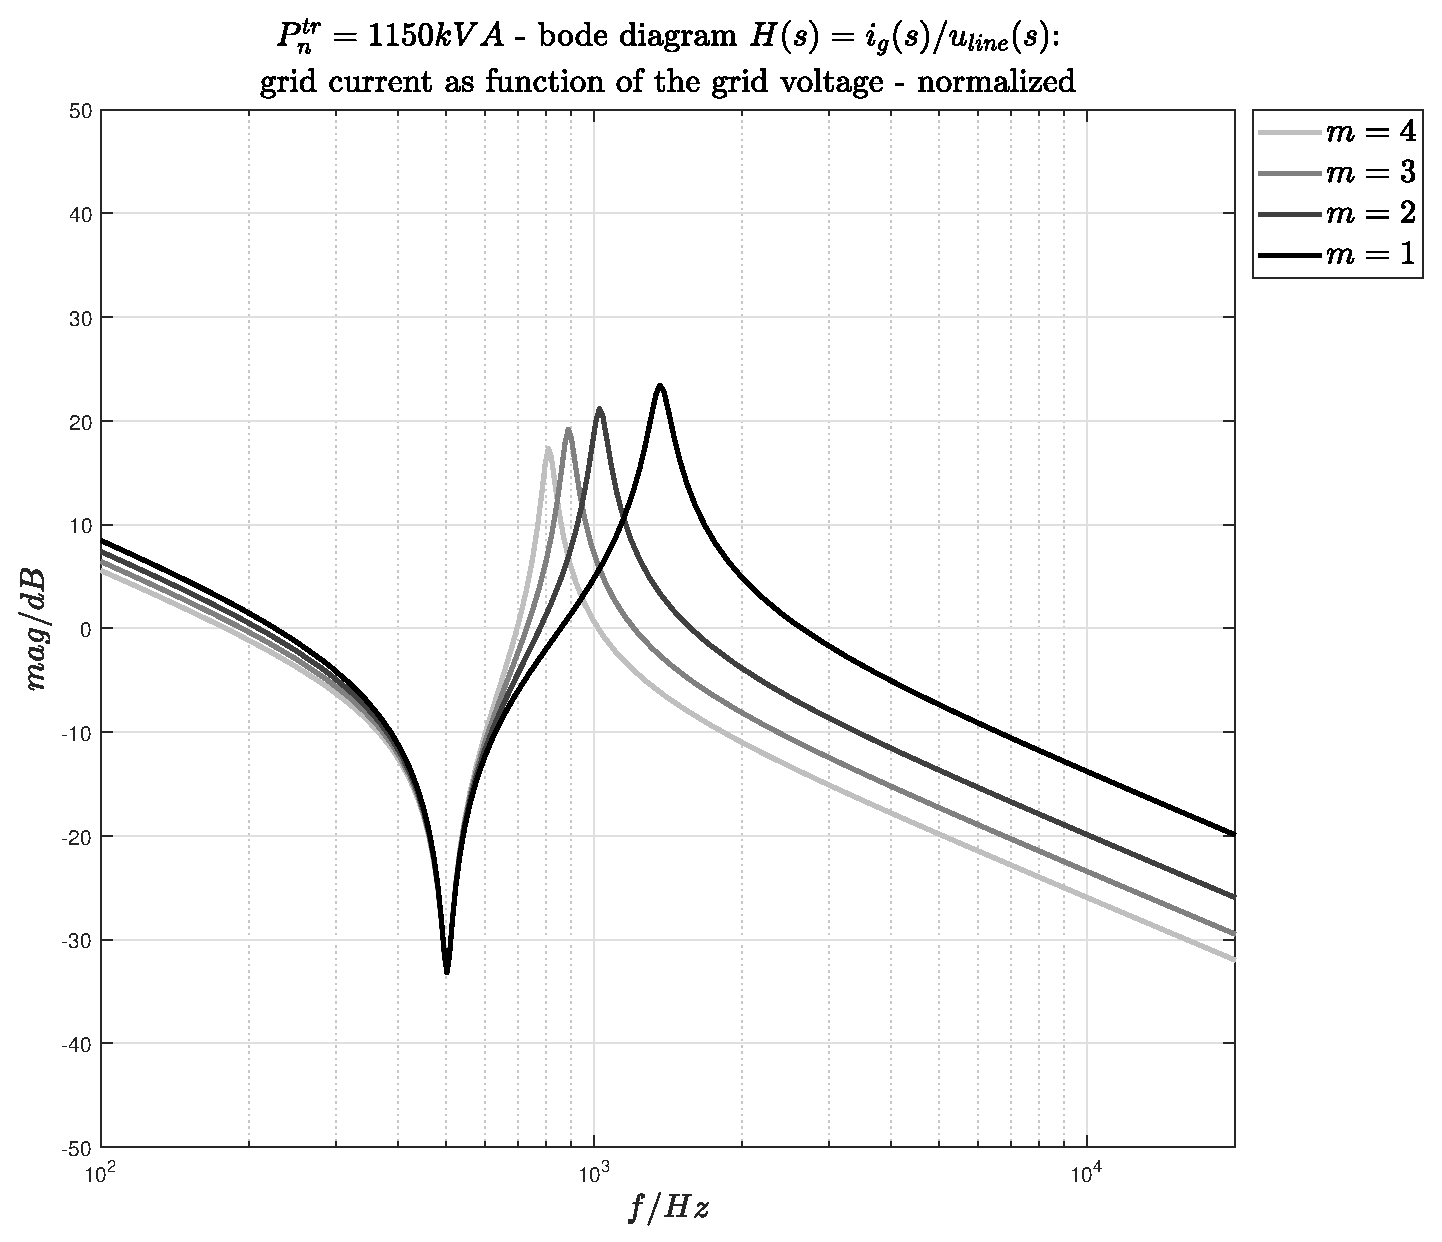
\includegraphics[width =250pt, angle = 0, 
		keepaspectratio]{figures/output_filter_analysis/bode_analysis/bode_analysis_ig_ug_1150kVA.eps}
		\captionsetup{width=0.75\textwidth, font=footnotesize}	
		\caption{Bode diagram of the equivalent of the transfer function: ${i_g(s)}/{u_{line}(s)}$, for $m=1,2,3,4$ modules connected to the grid via a transformer of $P_n=\SI{1150}{\kilo{\volt\ampere}}$.}
		\label{bode_analysis_ig_ug_1150kVA}
	\end{subfigure}
	\begin{subfigure}{0.5\textwidth}
		\centering
		\includegraphics[width =250pt, angle = 0, 
		keepaspectratio]{figures/output_filter_analysis/bode_analysis/bode_analysis_ig_us_1150kVA.eps}
		\captionsetup{width=0.75\textwidth, font=footnotesize}	
		\caption{Bode diagram of the equivalent of the transfer function: ${i_g(s)}/{u_{s}(s)}$, for $m=1,2,3,4$ modules connected to the grid via a transformer of $P_n=\SI{1150}{\kilo{\volt\ampere}}$.}
		\label{bode_analysis_ig_us_1150kVA}
	\end{subfigure}
	\captionsetup{width=0.65\textwidth, font=small}	
	\caption{Bode diagrams of  ${i_g(s)}/{i_{s}(s)}$, ${i_g(s)}/{u_{line}(s)}$, and ${i_g(s)}/{u_{s}(s)}$  transfer functions of the system \textit{grid/transformer/output-filter/AFE-VSI} for $m=1,2,3,4$ modules connected to the grid via a transformer of $P_n=\SI{1150}{\kilo{\volt\ampere}}$.}
	\label{bode_analysis_1150kVA}
\end{figure}


\begin{figure}[H]
	\centering
	\begin{subfigure}{0.5\textwidth}
		\centering
		\includegraphics[width =250pt, angle = 0, 
		keepaspectratio]{figures/output_filter_analysis/bode_analysis/bode_analysis_ig_is_1670kVA.eps}
		\captionsetup{width=0.65\textwidth, font=footnotesize}	
		\caption{Bode diagram of the equivalent of the transfer function: ${i_g(s)}/{i_{s}(s)}$, for $m=1,2,4,6$ modules connected to the grid via a transformer of $P_n=\SI{1670}{\kilo{\volt\ampere}}$.}
		\label{bode_analysis_ig_is_1670kVA}
	\end{subfigure}%
	\begin{subfigure}{0.5\textwidth}
		\centering
		\includegraphics[width =250pt, angle = 0, 
		keepaspectratio]{figures/output_filter_analysis/bode_analysis/bode_analysis_ig_ug_1670kVA.eps}
		\captionsetup{width=0.75\textwidth, font=footnotesize}	
		\caption{Bode diagram of the equivalent of the transfer function: ${i_g(s)}/{u_{line}(s)}$, for $m=1,2,4,6$ modules connected to the grid via a transformer of $P_n=\SI{1670}{\kilo{\volt\ampere}}$.}
		\label{bode_analysis_ig_ug_1670kVA}
	\end{subfigure}
	\begin{subfigure}{0.5\textwidth}
		\centering
		\includegraphics[width =250pt, angle = 0, 
		keepaspectratio]{figures/output_filter_analysis/bode_analysis/bode_analysis_ig_us_1670kVA.eps}
		\captionsetup{width=0.75\textwidth, font=footnotesize}	
		\caption{Bode diagram of the equivalent of the transfer function: ${i_g(s)}/{u_{s}(s)}$, for $m=1,2,4,6$ modules connected to the grid via a transformer of $P_n=\SI{1670}{\kilo{\volt\ampere}}$.}
		\label{bode_analysis_ig_us_1670kVA}
	\end{subfigure}
	\captionsetup{width=0.65\textwidth, font=small}	
	\caption{Bode diagrams of  ${i_g(s)}/{i_{s}(s)}$, ${i_g(s)}/{u_{line}(s)}$, and ${i_g(s)}/{u_{s}(s)}$  transfer functions of the system \textit{grid/transformer/output-filter/AFE-VSI} for $m=1,2,3,4$ modules connected to the grid via a transformer of $P_n=\SI{1670}{\kilo{\volt\ampere}}$.}
	\label{bode_analysis_1670kVA}
\end{figure}

\begin{figure}[H]
	\centering
	\begin{subfigure}{0.5\textwidth}
		\centering
		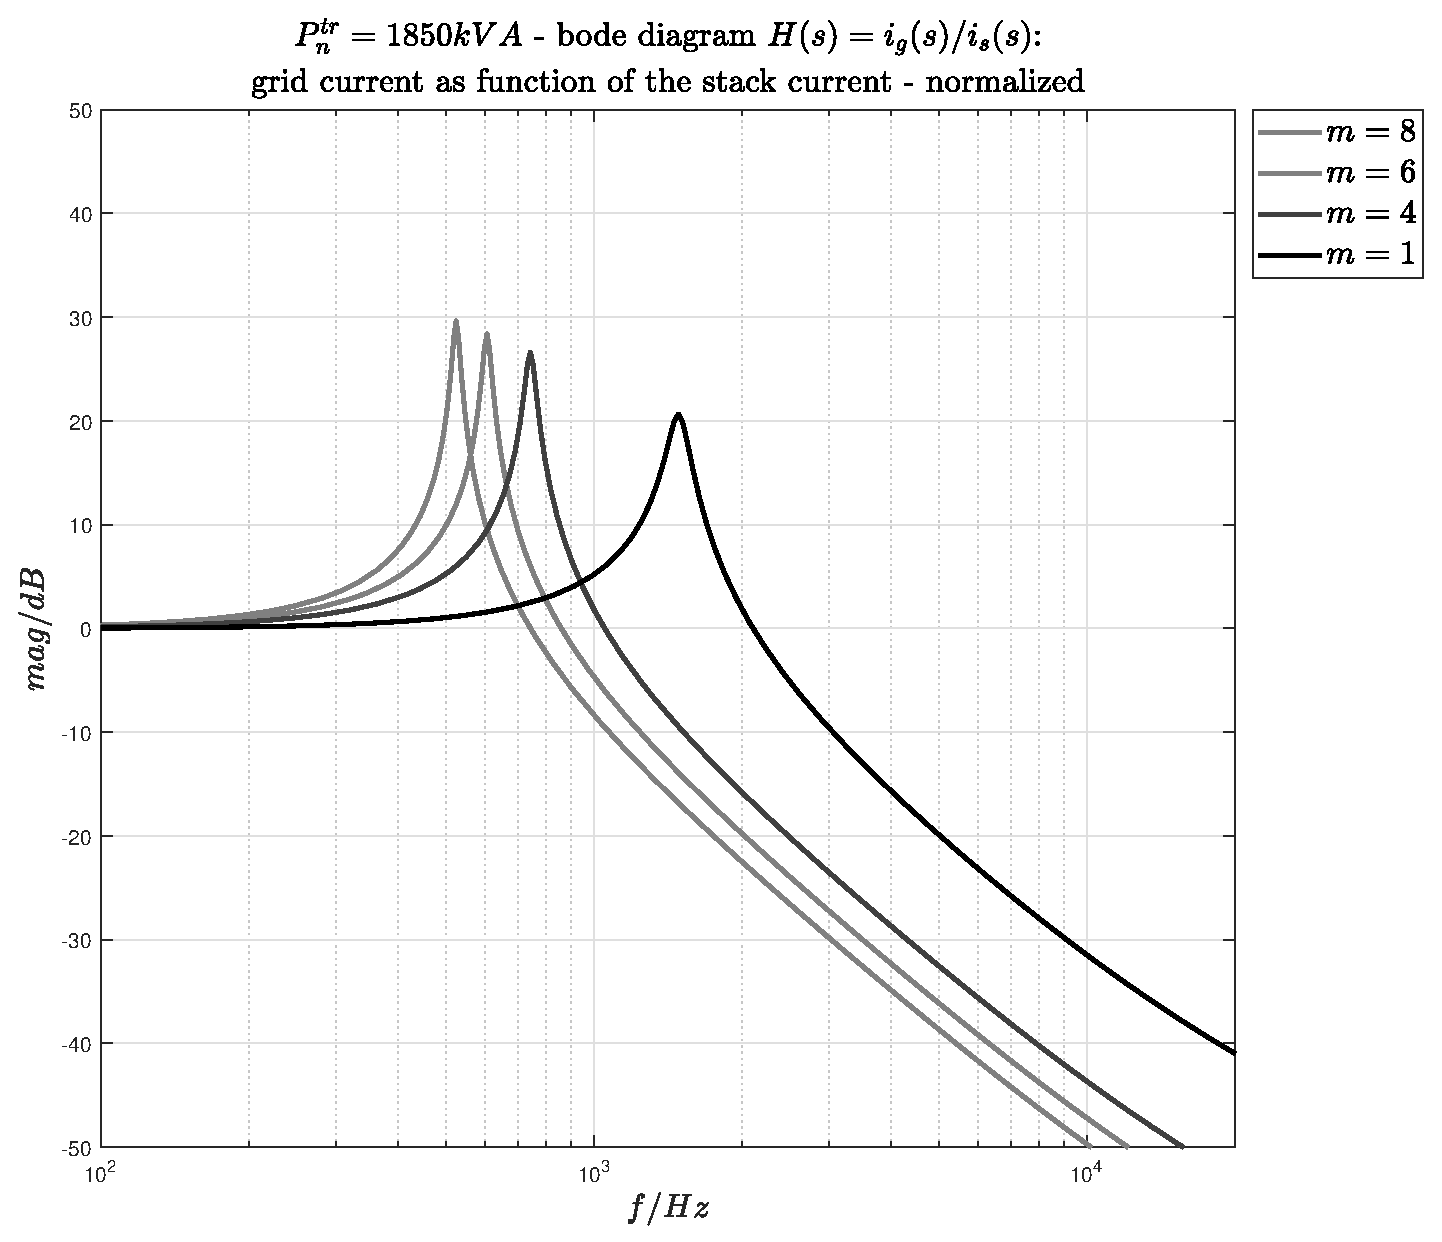
\includegraphics[width =250pt, angle = 0, 
		keepaspectratio]{figures/output_filter_analysis/bode_analysis/bode_analysis_ig_is_1850kVA.eps}
		\captionsetup{width=0.65\textwidth, font=footnotesize}	
		\caption{Bode diagram of the equivalent of the transfer function: ${i_g(s)}/{i_{s}(s)}$, for $m=1,4,6,8$ modules connected to the grid via a transformer of $P_n=\SI{1850}{\kilo{\volt\ampere}}$.}
		\label{bode_analysis_ig_is_1850kVA}
	\end{subfigure}%
	\begin{subfigure}{0.5\textwidth}
		\centering
		\includegraphics[width =250pt, angle = 0, 
		keepaspectratio]{figures/output_filter_analysis/bode_analysis/bode_analysis_ig_ug_1850kVA.eps}
		\captionsetup{width=0.75\textwidth, font=footnotesize}	
		\caption{Bode diagram of the equivalent of the transfer function: ${i_g(s)}/{u_{line}(s)}$, for $m=1,4,6,8$ modules connected to the grid via a transformer of $P_n=\SI{1850}{\kilo{\volt\ampere}}$.}
		\label{bode_analysis_ig_ug_1850kVA}
	\end{subfigure}
	\begin{subfigure}{0.5\textwidth}
		\centering
		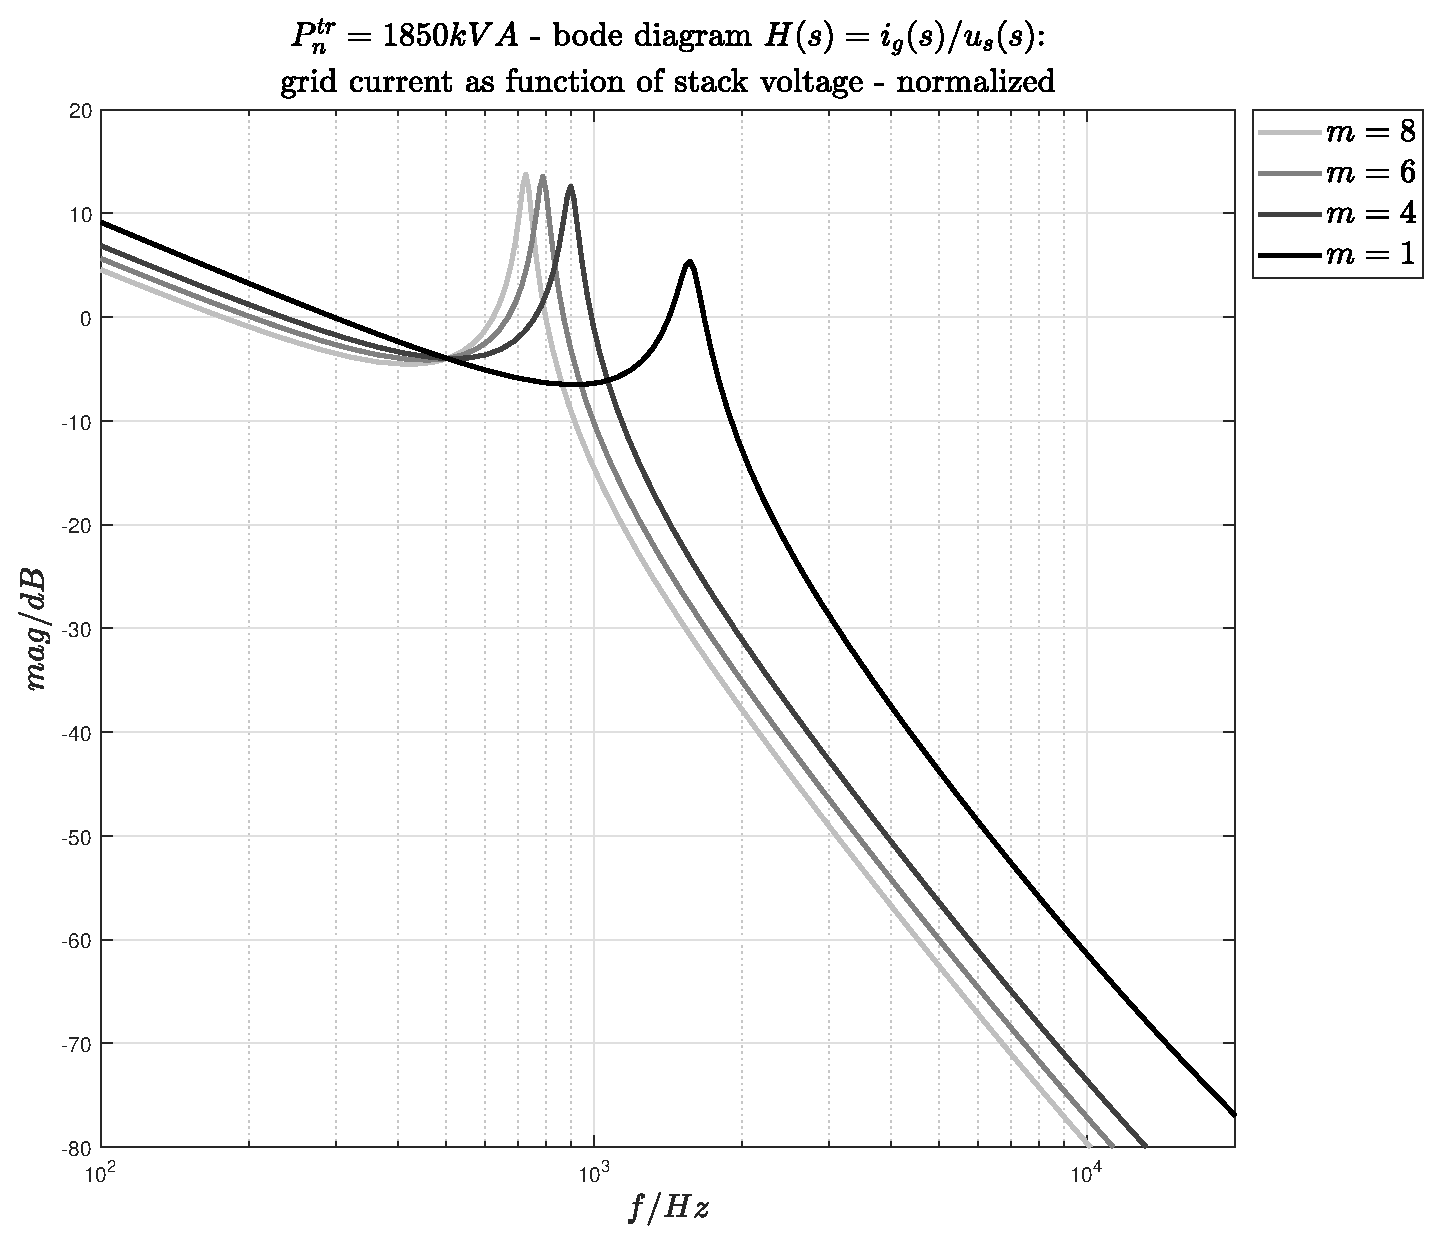
\includegraphics[width =250pt, angle = 0, 
		keepaspectratio]{figures/output_filter_analysis/bode_analysis/bode_analysis_ig_us_1850kVA.eps}
		\captionsetup{width=0.75\textwidth, font=footnotesize}	
		\caption{Bode diagram of the equivalent of the transfer function: ${i_g(s)}/{u_{s}(s)}$, for $m=1,4,6,8$ modules connected to the grid via a transformer of $P_n=\SI{1850}{\kilo{\volt\ampere}}$.}
		\label{bode_analysis_ig_us_1850kVA}
	\end{subfigure}
	\captionsetup{width=0.65\textwidth, font=small}	
	\caption{Bode diagrams of  ${i_g(s)}/{i_{s}(s)}$, ${i_g(s)}/{u_{line}(s)}$, and ${i_g(s)}/{u_{s}(s)}$  transfer functions of the system \textit{grid/transformer/output-filter/AFE-VSI} for $m=1,2,3,4$ modules connected to the grid via a transformer of $P_n=\SI{1850}{\kilo{\volt\ampere}}$.}
	\label{bode_analysis_1850kVA}
\end{figure}

\begin{figure}[H]
	\centering
	\begin{subfigure}{0.5\textwidth}
		\centering
		\includegraphics[width =250pt, angle = 0, 
		keepaspectratio]{figures/output_filter_analysis/bode_analysis/bode_analysis_ig_us_1150kVA.eps}
		\captionsetup{width=0.75\textwidth, font=footnotesize}	
		\caption{Bode diagram of the equivalent of the transfer function: ${i_g(s)}/{u_{s}(s)}$, for $m=1,2,3,4$ modules connected to the grid via a transformer of $P_n=\SI{1150}{\kilo{\volt\ampere}}$.}
		\label{}
	\end{subfigure}%
	\begin{subfigure}{0.5\textwidth}
		\centering
		\includegraphics[width =250pt, angle = 0, 
		keepaspectratio]{figures/output_filter_analysis/bode_analysis/bode_analysis_ig_us_1670kVA.eps}
		\captionsetup{width=0.75\textwidth, font=footnotesize}	
		\caption{Bode diagram of the equivalent of the transfer function: ${i_g(s)}/{u_{s}(s)}$, for $m=1,4,6,8$ modules connected to the grid via a transformer of $P_n=\SI{1670}{\kilo{\volt\ampere}}$.}
		\label{}
	\end{subfigure}
	\begin{subfigure}{0.5\textwidth}
		\centering
		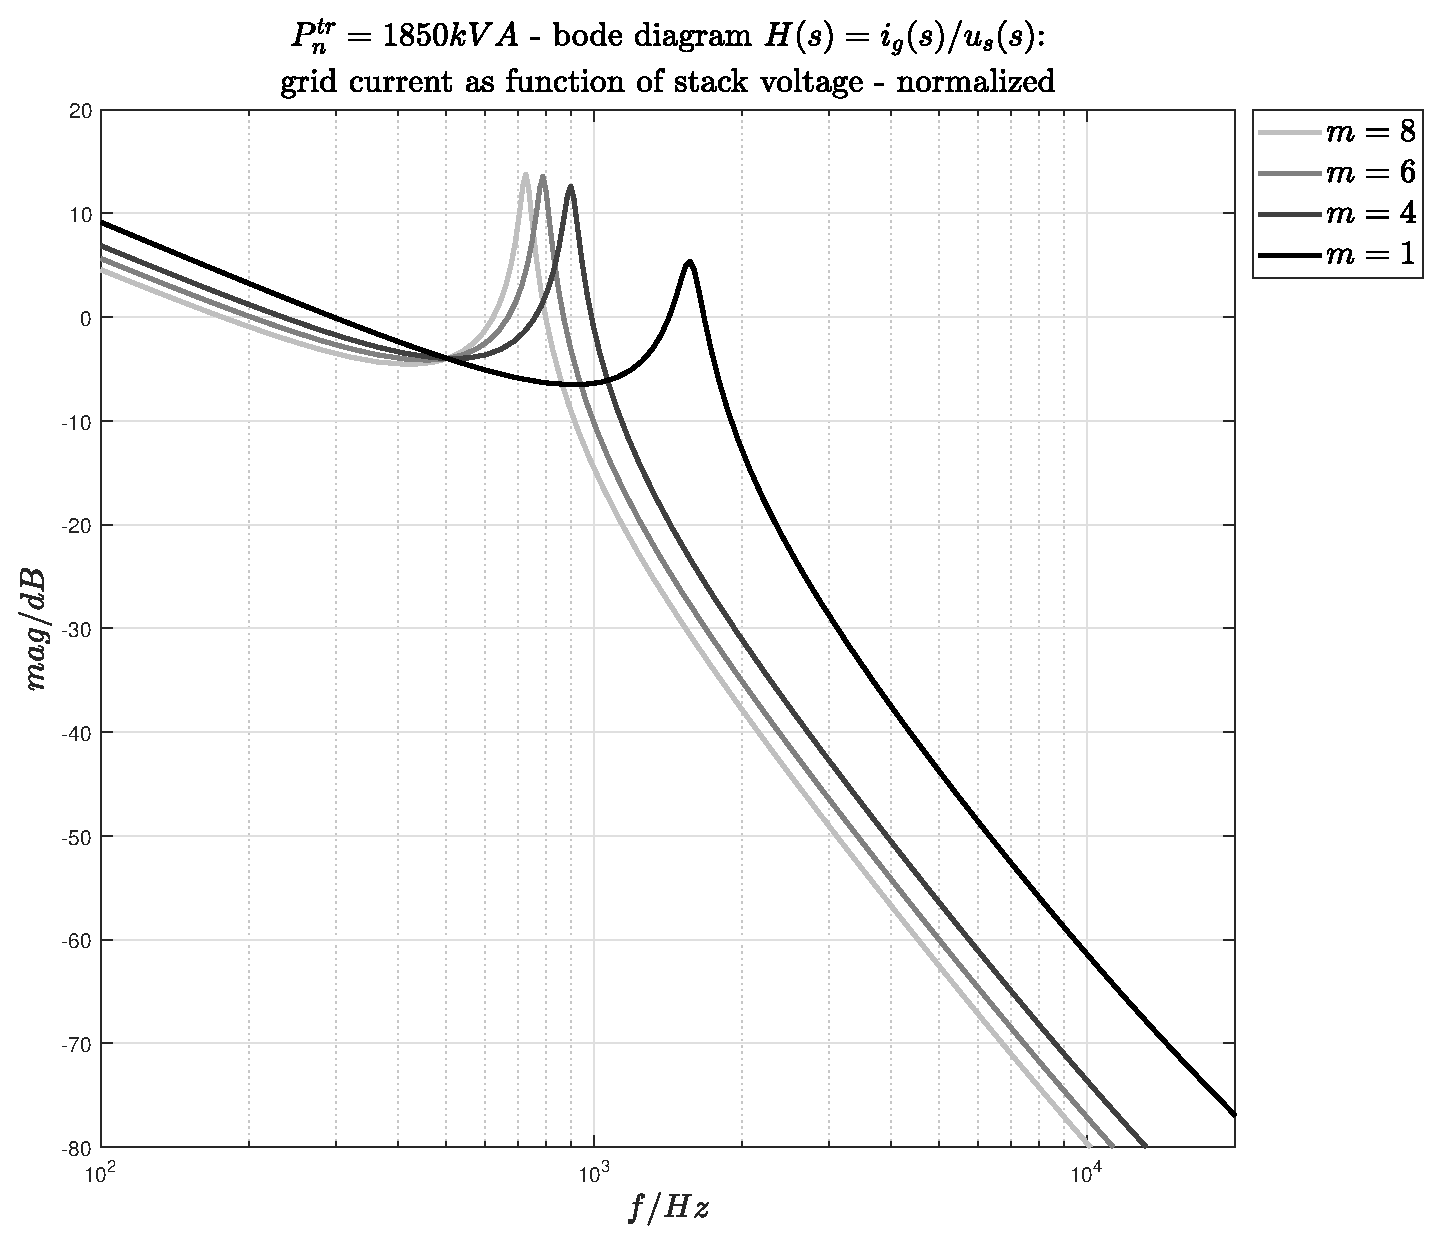
\includegraphics[width =250pt, angle = 0, 
		keepaspectratio]{figures/output_filter_analysis/bode_analysis/bode_analysis_ig_us_1850kVA.eps}
		\captionsetup{width=0.75\textwidth, font=footnotesize}	
		\caption{Bode diagram of the equivalent of the transfer function: ${i_g(s)}/{u_{s}(s)}$, for $m=1,4,6,8$ modules connected to the grid via a transformer of $P_n=\SI{1850}{\kilo{\volt\ampere}}$.}
		\label{}
	\end{subfigure}
	\captionsetup{width=0.65\textwidth, font=small}	
	\caption{Bode diagrams of ${i_g(s)}/{u_{s}(s)}$ transfer function for different equivalent grid impedance $L_g$ (or $P_n$) values, and different number of  parallelised \textit{ElectricalDrive}.}
	\label{bode_analysis_1150kVA_1850kVA}
\end{figure}

\section{Case scenario of one \textit{ElectricalDrive}: benchmark}
In order to investigate the impact of the modularity, a case scenario composed by a single \textit{ElectricalDrive} connected to a $i_{cc}=\SI{50}{\kilo\ampere}$ power grid by a MV/LV transformer with a nominal power of $P_n=\SI{1150}{\kilo{\volt\ampere}}$, see Figure~\ref{one_ElectricalDrive_benchmark}, will be initially investigated. These results will be used as benchmark for the rest of all cases scenario analysis.
\begin{figure}[H]
	\centering
	\includegraphics[width = 500pt, angle = 0, 
	keepaspectratio]{figures/one_ElectricalDrive_benchmark.eps}
	\captionsetup{width=0.75\textwidth, font=small}	
	\caption{One \textit{ElectricalDrive} case scenario used as benchmark for further investigation on modularity effect on grid power quality. As shown in the figure, a $i_{cc}=\SI{50}{\kilo\ampere}$ power grid has been assumed, a $P_n=\SI{1150}{\kilo{\volt\ampere}}$ MV/LV and an equivalent PSM three phase system with a nominal power of 250kW and a nominal current of 370A (rms). For sake of clarity. simulations have been performed supposing the grid line voltage affected by a 1\% of fifth voltage harmonics as well as PSM back EMF voltage is assumed affected by a 2\% of fifth voltage harmonic.}
	\label{one_ElectricalDrive_benchmark}
\end{figure}


 \begin{center}	
	\onehalfspacing
	\begin{longtable}{p{0.4\linewidth}|p{0.15\linewidth}|p{0.35\linewidth}}
		\captionsetup{width=.5\textwidth, font=small}
		\caption{PSM three-phase system data used for the single \textit{ElectricalDrive} case scenario.}
		\label{motor_data_single_ElectricalDrive_case_scenario} \\
		\hline\hline
		\textbf{data} & \textbf{value} & \textbf{comment} \\
		\hline
		{\fontfamily{cmss}\selectfont \verb+nominal RPM+} : \hspace*{\fill} $\omega_m^{nom}$ & \hspace*{\fill} $\SI{17.8}{\per\minute}$ & nominal mechanical rotor speed; \\	
		{\fontfamily{cmss}\selectfont \verb+number of pole pairs+}: \hspace*{\fill} $p$ & \hspace*{\fill} $\SI{52}{}$ & number of pole pairs;\\		
		{\fontfamily{cmss}\selectfont \verb+nominal phase current+}: \hspace*{\fill} $I^{nom}$ & \hspace*{\fill} $\SI{344.0}{\ampere}$ & nominal phase current in rms; \\	
		{\fontfamily{cmss}\selectfont \verb+self inductance+}: \hspace*{\fill} $L_a$ & \hspace*{\fill} $\SI{4.6}{\milli\henry}$ & self inductance, used into matrix inductance; \\	
		{\fontfamily{cmss}\selectfont \verb+mutual inductance+}: \hspace*{\fill} $L_b$ & \hspace*{\fill} $\SI{4.4}{\milli\henry}$ & mutual inductance, used into matrix inductance; \\		
		{\fontfamily{cmss}\selectfont \verb+nominal rotor pm flux+}: \hspace*{\fill} $\psi^m$ & \hspace*{\fill} $\SI{3.84}{\volt\second}$ & permanent magnet per-phase rotor flux linkage to the stator; \\	
		{\fontfamily{cmss}\selectfont \verb+fifth harmonic flux distortion+}: \hspace*{\fill} $h_5$ & \hspace*{\fill} $\SI{2}{\percent}$ & spatial fifth harmonic distortion of the back EMF.\\	
		\hline
	\end{longtable}
\end{center}

 \begin{center}	
	\onehalfspacing
	\begin{longtable}{p{0.35\linewidth}|p{0.15\linewidth}|p{0.4\linewidth}}
		\captionsetup{width=.5\textwidth, font=small}
		\caption{Grid and MV/LV equivalent data used for the single \textit{ElectricalDrive} case scenario.}
		\label{grid_and_transformer_data_single_ElectricalDrive_case_scenario} \\
		\hline\hline
		\textbf{data} & \textbf{value} & \textbf{comment} \\
		\hline
		{\fontfamily{cmss}\selectfont \verb+LV nominal voltage+} : \hspace*{\fill} $U_2$ & \hspace*{\fill} $\SI{690}{\volt}$ & nominal voltage of the LV side; \\	
		{\fontfamily{cmss}\selectfont \verb+5th harmonic component+} : \hspace*{\fill} $U_{5}$ & \hspace*{\fill} $\SI{1}{\percent}$ & 5th grid harmonic voltage component in percentage of the nominal value; \\	
		{\fontfamily{cmss}\selectfont \verb+grid impedance+} : \hspace*{\fill} $L_{line}$ & \hspace*{\fill} $\SI{25.4}{\micro\henry}$ & equivalent grid impedance at LV side: here a $i_{cc}=\SI{50}{\kilo\ampere}$ power grid is assumed; \\	
		{\fontfamily{cmss}\selectfont \verb+nominal power of the TR+} : \hspace*{\fill} $P_n$ & \hspace*{\fill} $\SI{1150}{\kilo{\volt\ampere}}$ & nominal power of the MV/LV power transformer; \\	
		{\fontfamily{cmss}\selectfont \verb+TR leakage impedance+} : \hspace*{\fill} $L_\sigma$ & \hspace*{\fill} $\SI{79}{\micro\henry}$ & equivalent LV side leakage inductance of the MV/LV transformer assuming a $U_{cc} = \SI{6}{\percent}$; \\	
		\hline
	\end{longtable}
\end{center}

\subsection{Simulation results - benchmark}
The following simulation results concerns a case scenario of one \textit{ElectricalDrive} connected to a grid with a short circuit current capability of $i_{cc}=\SI{50}{\kilo\ampere}$\footnote{
Short circuit current and equivalent grid leakage inductance ($L_{line}$) are, along the document, correlated by the formula:
\begin{align}
	L_{line} &= \frac{U_{line}^{ph}}{\omega \ i_{cc}}  &&
\end{align}
} via a MV/LV transformer with a nominal power of $P_n = \SI{1150}{\kilo{\volt\ampere}}$. 

Additional constraints are below reported
\begin{itemize}
	\item[--] grid voltage source $\vec{u}_{line}^{\,abd}$ is supposed to be affected by a fifth harmonic component which amplitude is $U_{5}=\SI{1}{\percent}$;
	\item[--] PSM back EMF is supposed to be affected by a fifth harmonic component which amplitude is $E_{5}=\SI{2}{\percent}$;
	\item[--] PSM mechanical rotor speed is assumed rotating at $\omega_m(t) = \SI{18.0}{\per\minute}$;	
	\item[--] \textbf{Nominal grid current used for normalization} : $I_{g}^{nom}(t) = \SI{295.8}{\ampere}$;	
	\item[--] \textbf{Nominal grid voltage used for normalization} : $U_{g}^{nom}(t) = \SI{563.4}{\volt}$;	
\end{itemize} 

\noindent\textbf{Some remarks:}
\begin{itemize}
	\item[--] the presence of a fifth harmonic component into the grid voltage will generated a contribution into the fifth harmonic current component;
	\item[--] the presence of a fifth harmonic component into the rotor flux (linkage to the stator) will generate an harmonic component which is function of the PSM rotor speed, in other words the harmonic distortion will be frequency-varying and this distortion will propagate from machine to the grid;
	\item[--] the presence of a fifth harmonic component into the PSM back EMF is, in general, rotating in opposite direction respect to the fundamental electrical pulsation, and it will generate a \textbf{torque ripple} component, which pulsation corresponds to the sixth harmonic of the fundamental.
\end{itemize}

\textbf{Remark} - the presence of a fifth harmonic component into the PSM back EMF rotating in opposite direction respect to the fundamental it will generate an active power pulsation (visible e.g. at the DClink stage) at the frequency of six times the fundamental of the PSM electrical pulsation.
\begin{figure}[H]
	\centering
	\begin{subfigure}{0.5\textwidth}
		\centering
		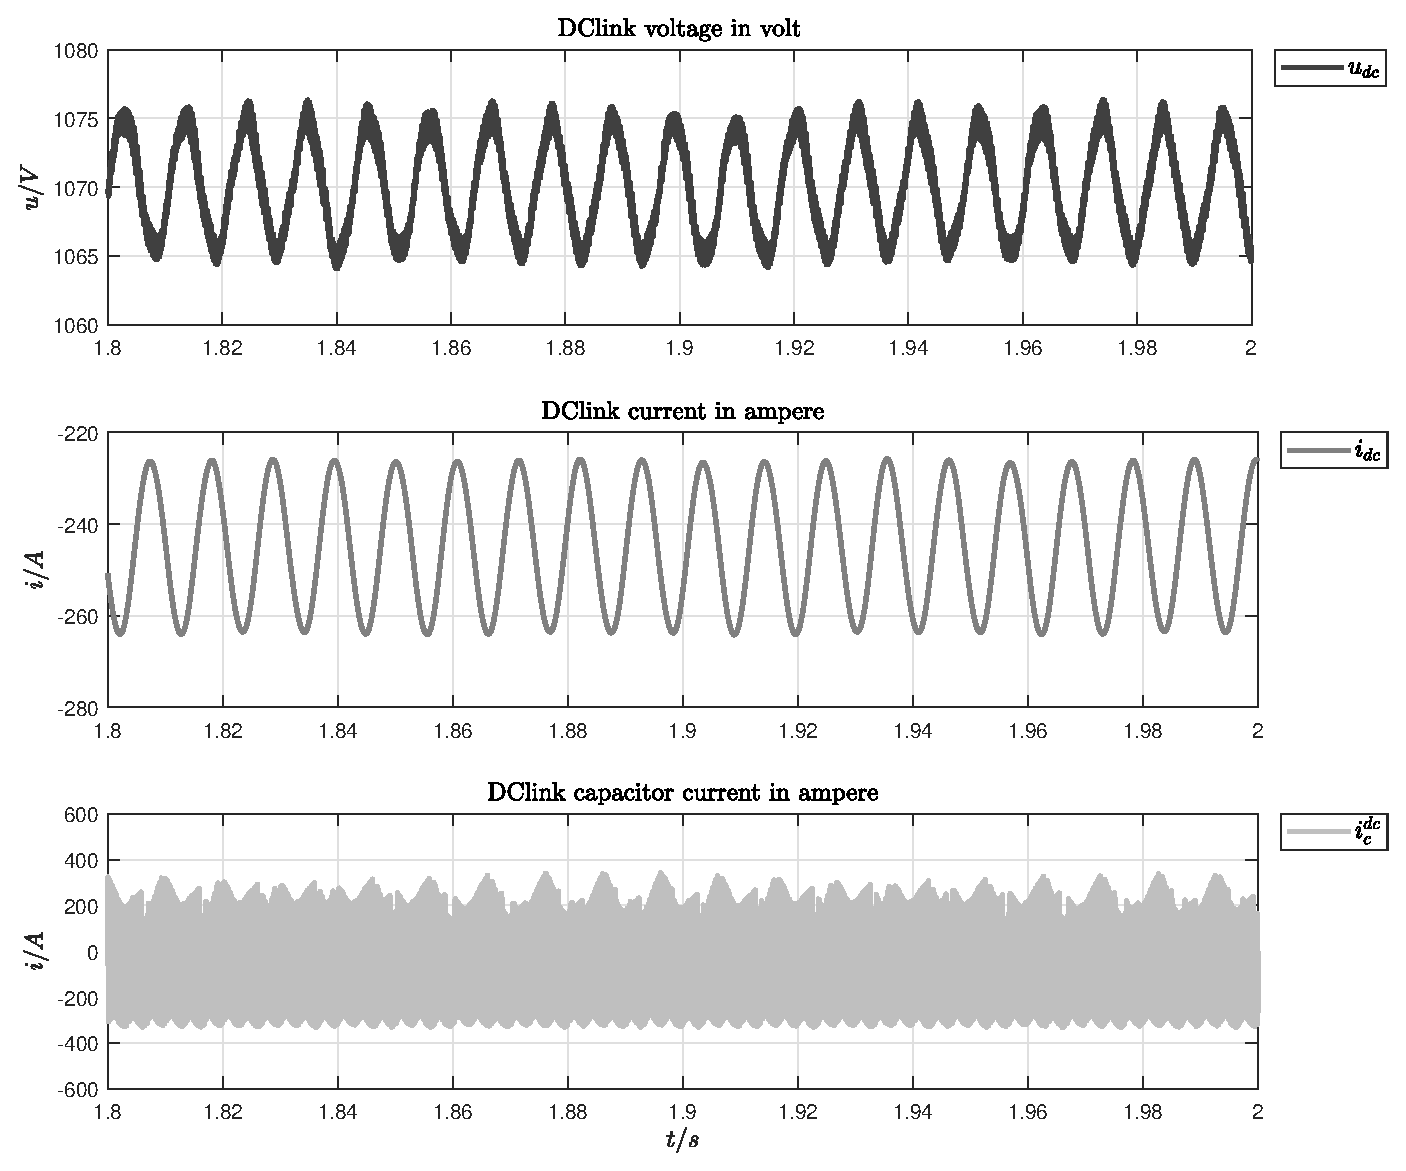
\includegraphics[width =225pt, angle = 0, 
		keepaspectratio]{figures/sim_results/benchmark_case_3/dclink_voltage_current.eps}
		\captionsetup{width=0.85\textwidth, font=footnotesize}	
		\caption{DClink voltage (top), DC-current at DClink stage (middle), and DClink capacitor current.}
		\label{benchmark_dclink_voltage_current}
	\end{subfigure}%
	\begin{subfigure}{0.5\textwidth}
		\centering
		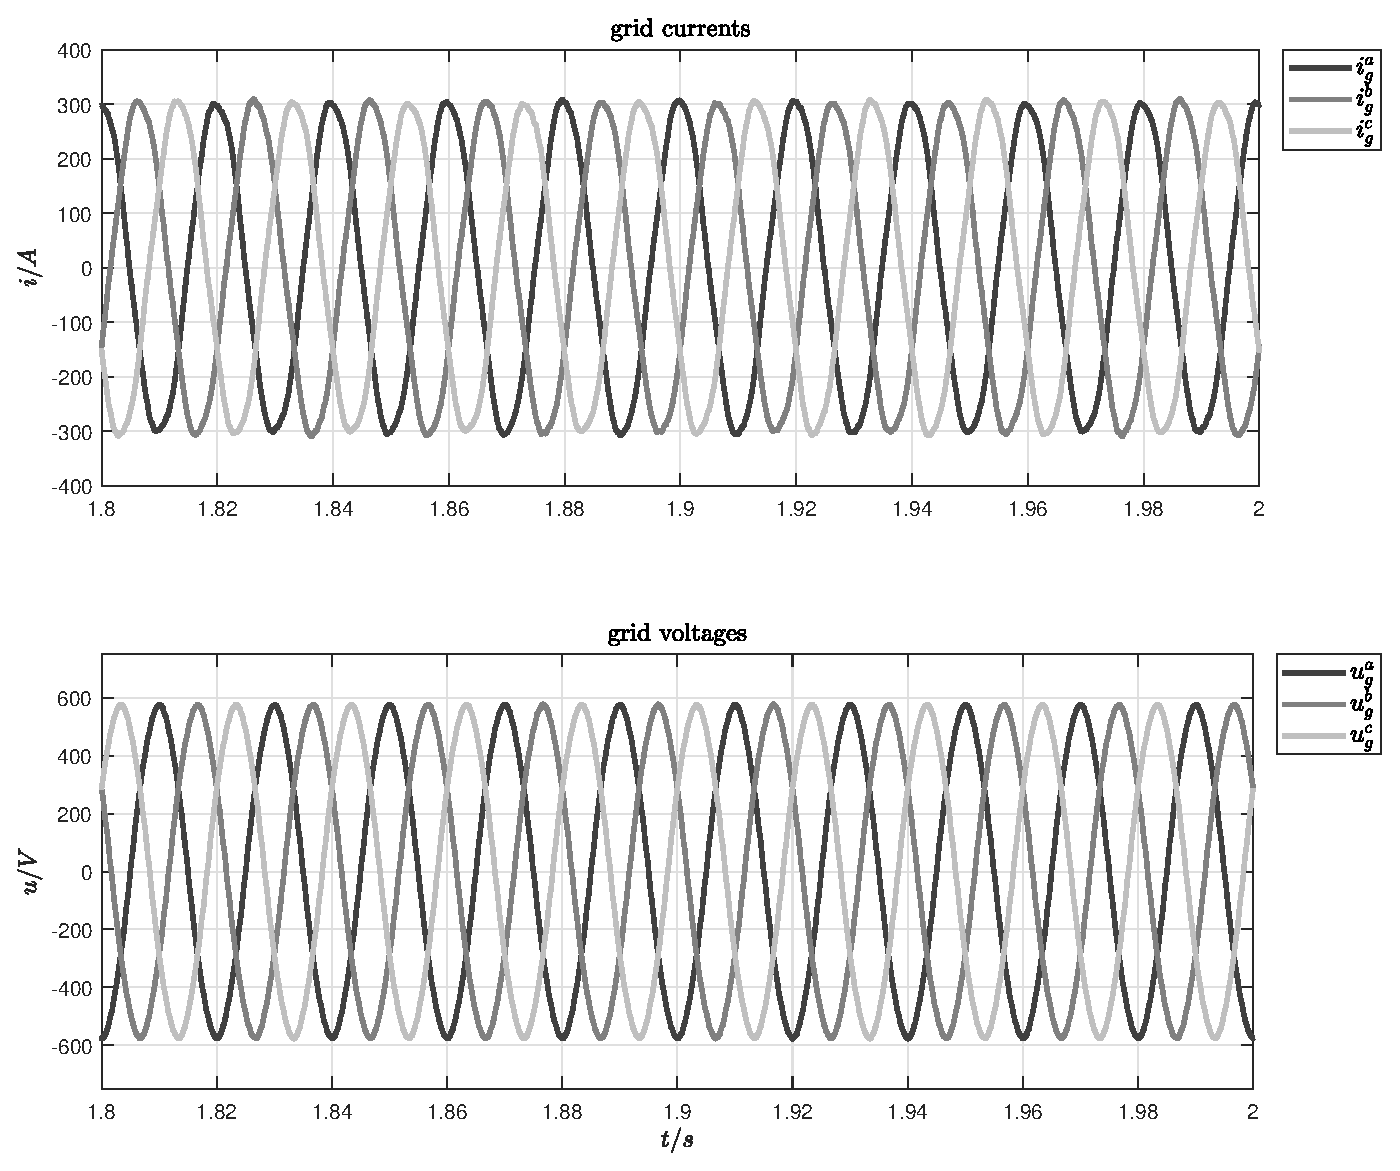
\includegraphics[width =225pt, angle = 0, 
		keepaspectratio]{figures/sim_results/benchmark_case_3/grid_voltages_currents.eps}
		\captionsetup{width=0.85\textwidth, font=footnotesize}	
		\caption{Grid electrical quantities, current (top) and voltage (bottom).}
		\label{}
	\end{subfigure}
	\captionsetup{width=0.65\textwidth, font=small}	
	\caption{DC-link and grid side quantities during nominal power condition for a single \textit{ElectricalDrive} connected to a $i_{cc} = \SI{50}{\kilo\ampere}$ grid with MV/LV transformer with a nominal power of $P_n = \SI{1150}{\kilo{\volt\ampere}}$. As shown in the figure (a), DClink voltage (and DC current) is affected by a sixth harmonic component ($\SI{93.6}{\hertz}$) of the electrical fundamental frequency ($\SI{15.6}{\hertz}$).}
	\label{}
\end{figure}

\begin{figure}[H]
	\centering
	\begin{subfigure}{0.5\textwidth}
		\centering
		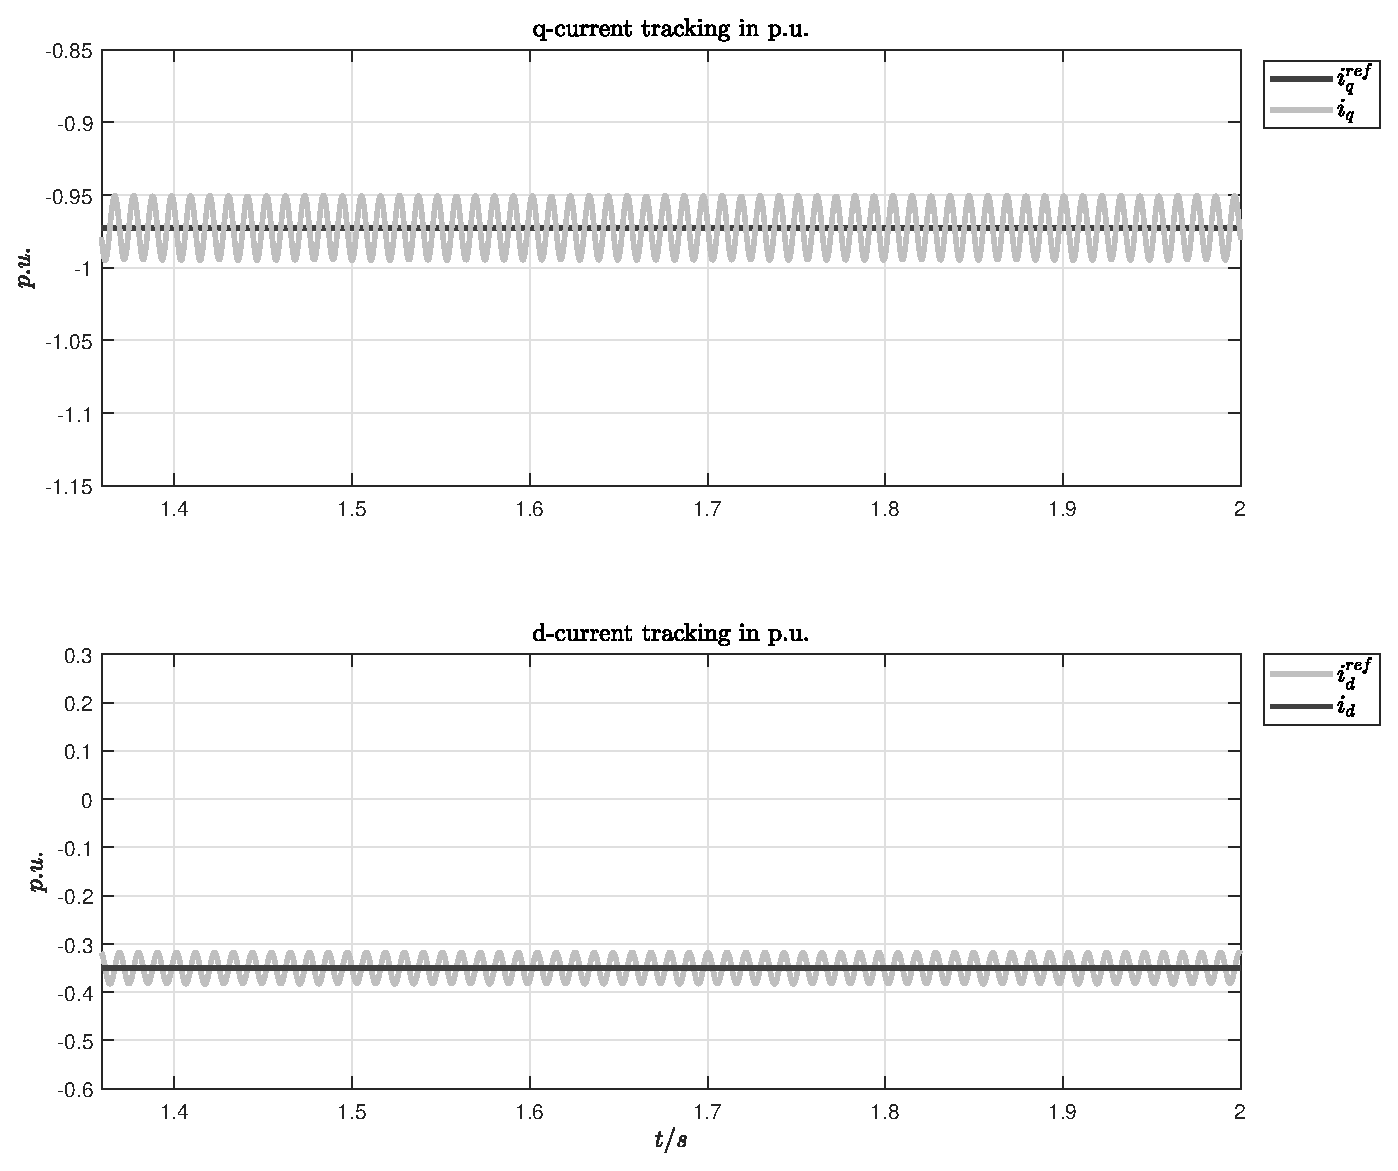
\includegraphics[width =225pt, angle = 0, 
		keepaspectratio]{figures/sim_results/benchmark_case_3/invert_current_control_quantities.eps}
		\captionsetup{width=0.85\textwidth, font=footnotesize}	
		\caption{vector current control tracking at machine side respect to the rotating reference frame: d-current (top), q-current (bottom), in per unit.}
		\label{}
	\end{subfigure}%
	\begin{subfigure}{0.5\textwidth}
		\centering
		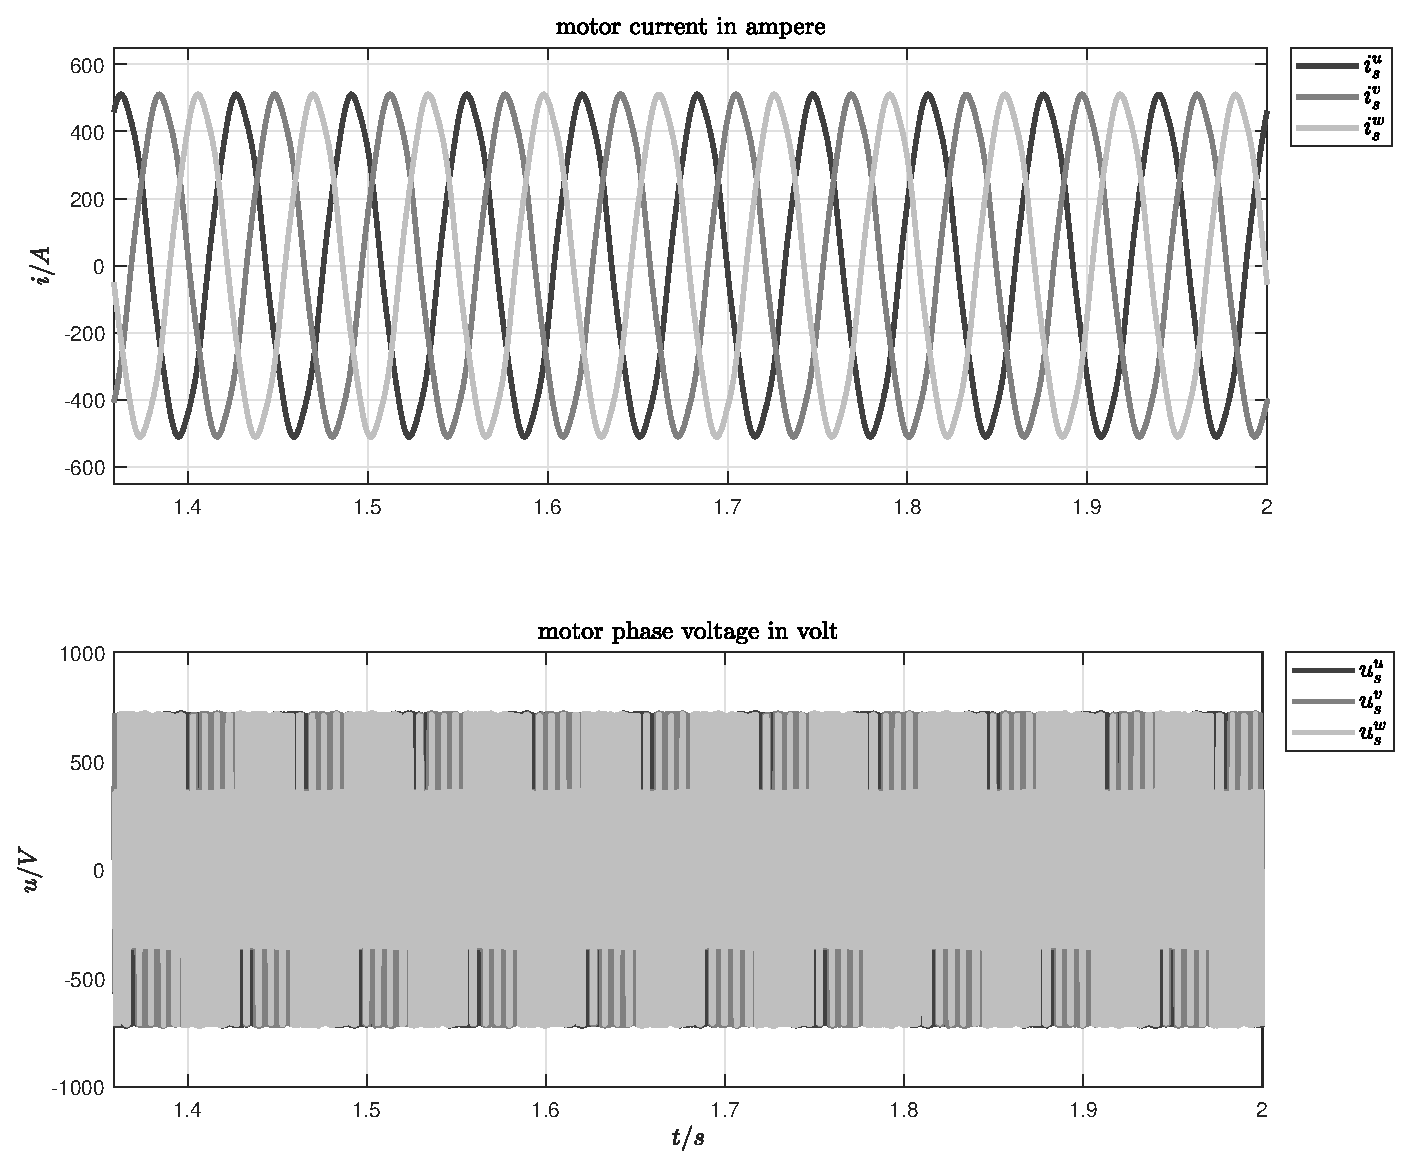
\includegraphics[width =225pt, angle = 0, 
		keepaspectratio]{figures/sim_results/benchmark_case_3/inverter_current_voltage.eps}
		\captionsetup{width=0.65\textwidth, font=footnotesize}	
		\caption{inverter output current and voltage respect to the stationary reference frame, in SI.}
		\label{}
	\end{subfigure}
	\captionsetup{width=0.65\textwidth, font=small}	
	\caption{Machine side quantities: inner current loop control (a), output current and voltage (b) during nominal power condition for a single \textit{ElectricalDrive} connected to a $i_{cc} = \SI{50}{\kilo\ampere}$ grid with MV/LV transformer with a nominal power of $P_n = \SI{1150}{\kilo{\volt\ampere}}$.}
	\label{}
\end{figure}

\begin{figure}[H]
	\centering
	\begin{subfigure}{0.5\textwidth}
		\centering
		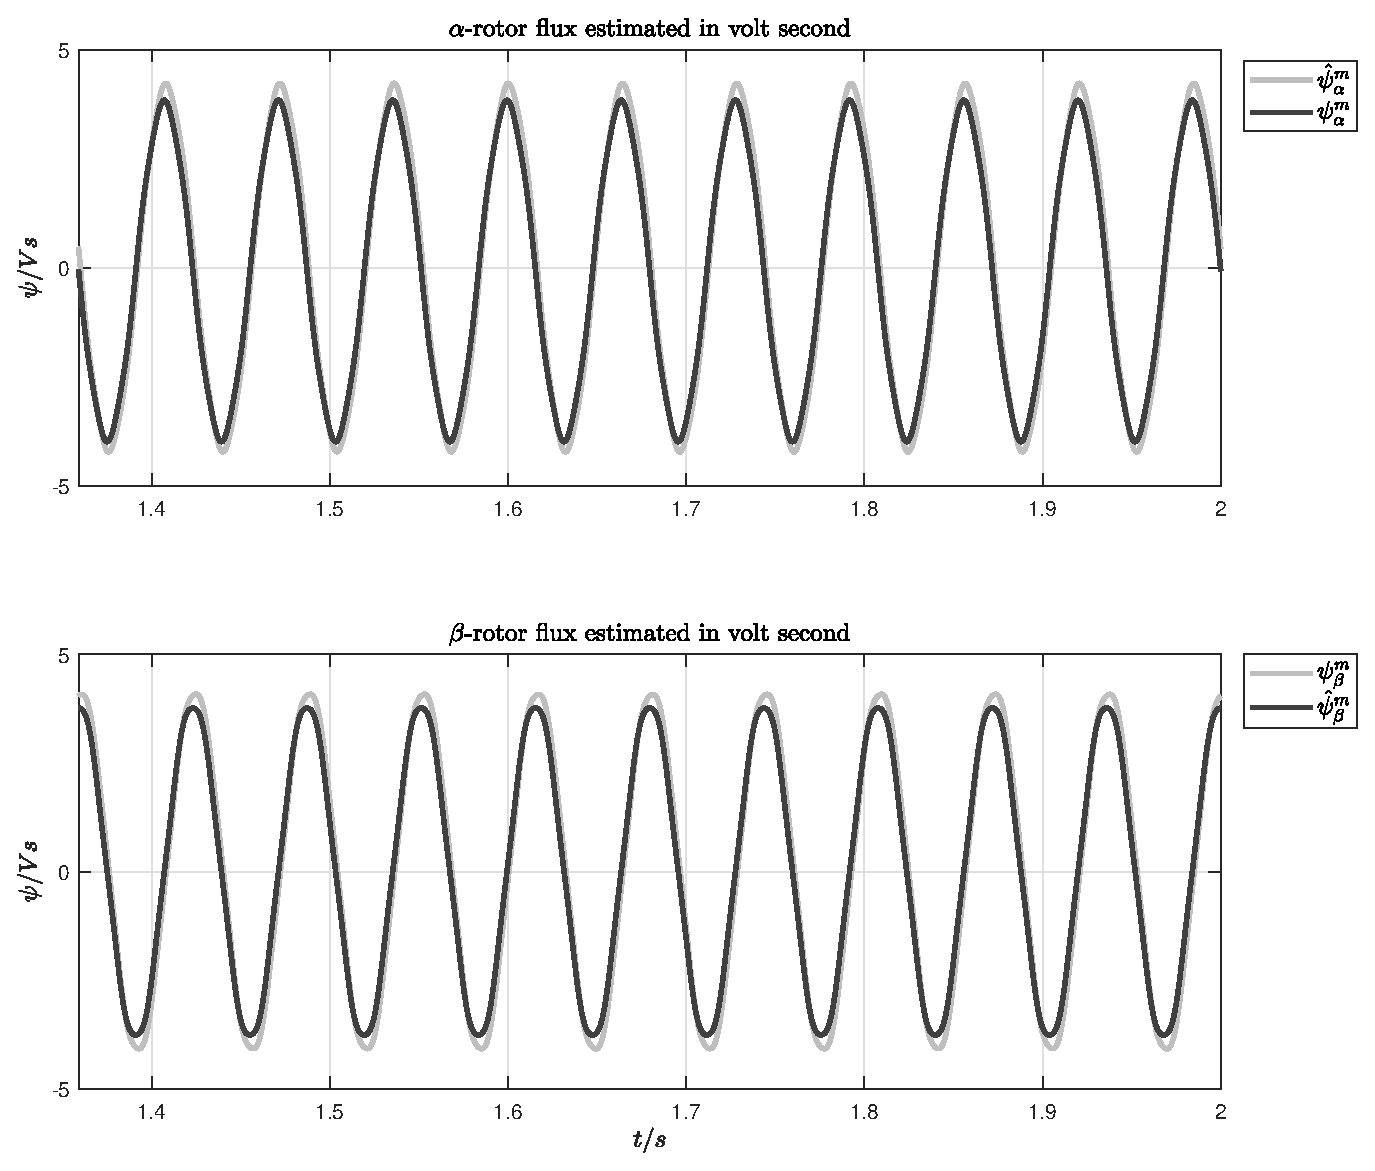
\includegraphics[width =225pt, angle = 0, 
		keepaspectratio]{figures/sim_results/benchmark_case_3/inverter_flux_observer.eps}
		\captionsetup{width=0.5\textwidth, font=footnotesize}	
		\caption{machine rotor flux (dark gray) and estimated (light gray) - $\alpha$-component (top), $\beta$-component (bottom).}
		\label{}
	\end{subfigure}%
	\begin{subfigure}{0.5\textwidth}
		\centering
		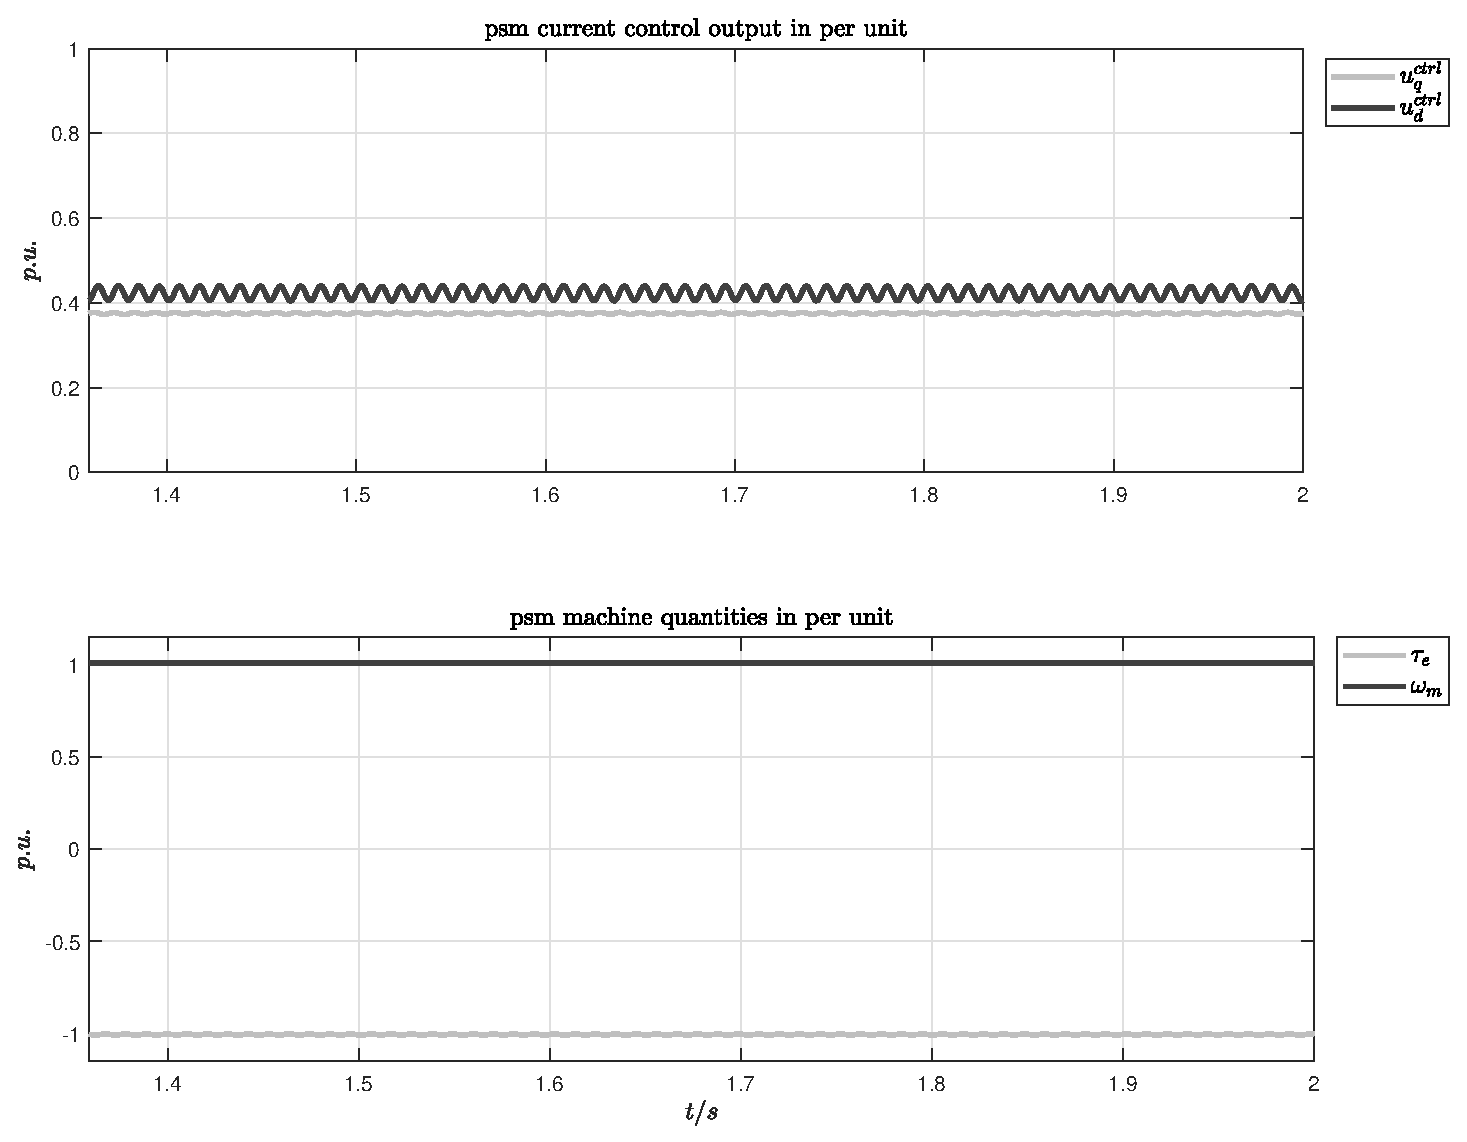
\includegraphics[width =225pt, angle = 0, 
		keepaspectratio]{figures/sim_results/benchmark_case_3/inverter_machine_quantities.eps}
		\captionsetup{width=0.95\textwidth, font=footnotesize}	
		\caption{per unit output current control loop: $u_d^{ctrl}(k)$, $u_q^{ctrl}(k)$ respect to the rotating reference frame (top); per unit mechanical quantities: rotor speed and electromechanical torque (bottom).}
		\label{}
	\end{subfigure}
	\captionsetup{width=0.65\textwidth, font=small}	
	\caption{inverter side per unit quantities, during nominal power condition for a single \textit{ElectricalDrive} connected to a $i_{cc} = \SI{50}{\kilo\ampere}$ grid with MV/LV transformer with a nominal power of $P_n = \SI{1150}{\kilo{\volt\ampere}}$.}
	\label{}
\end{figure}

\begin{figure}[H]
	\centering
	\begin{subfigure}{0.5\textwidth}
		\centering
		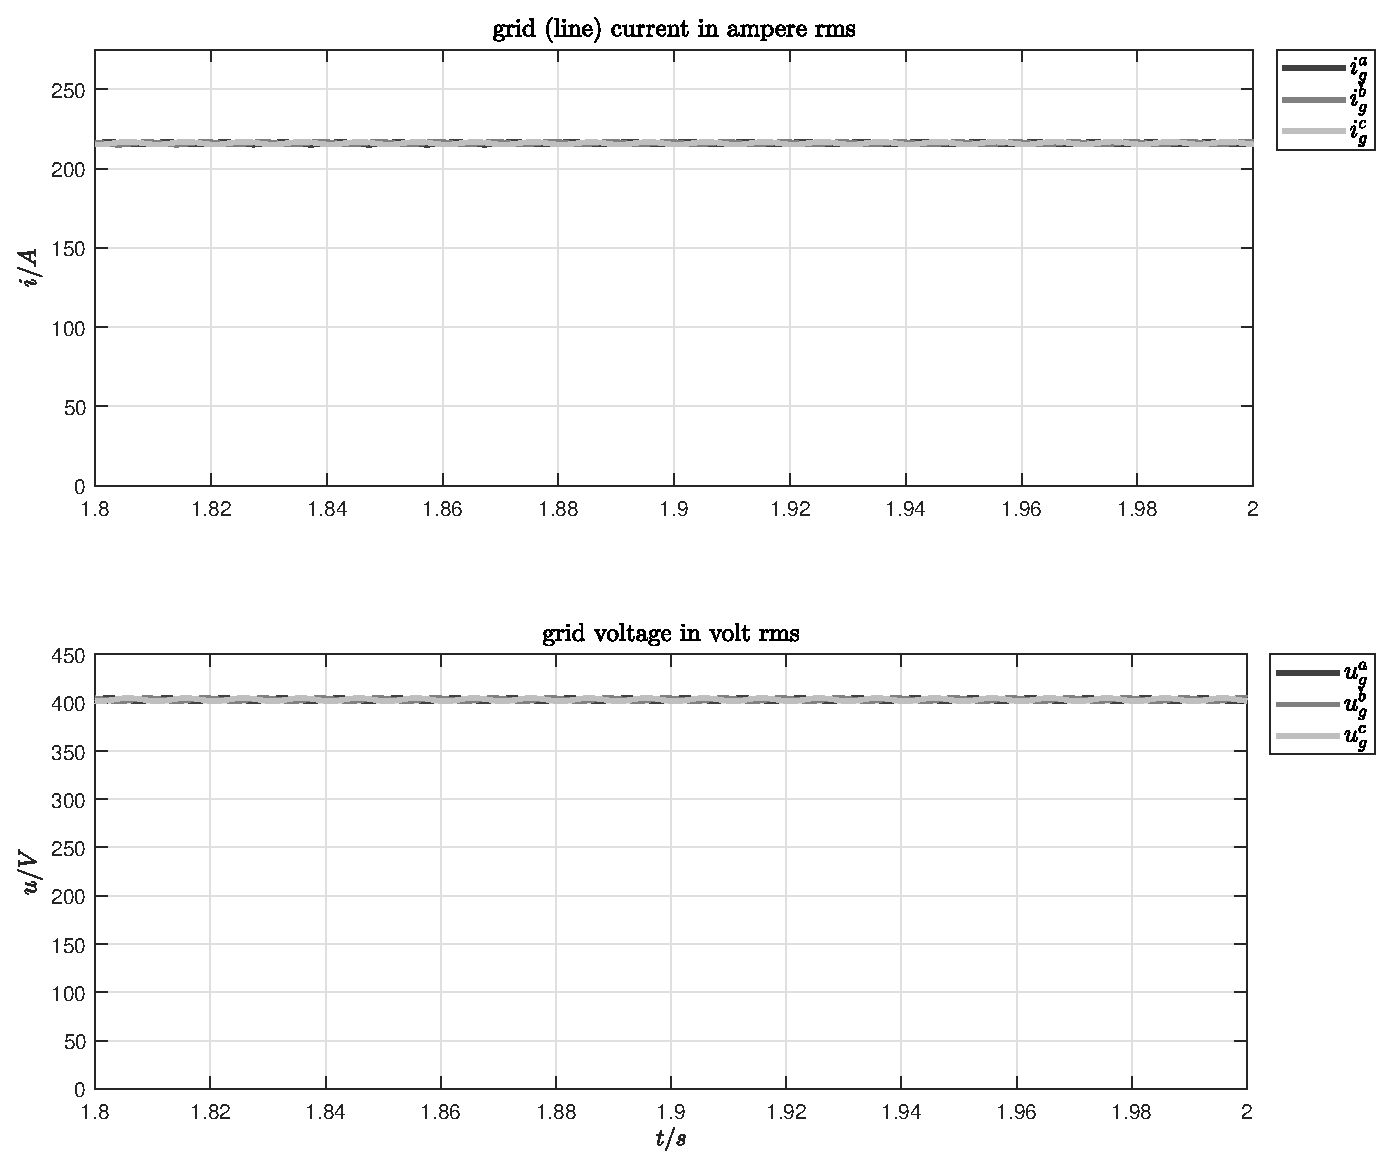
\includegraphics[width =225pt, angle = 0, 
		keepaspectratio]{figures/sim_results/benchmark_case_3/line_voltage_current_rms.eps}
		\captionsetup{width=0.5\textwidth, font=footnotesize}	
		\caption{grid side rms quantities: current rms (top), voltage rms (bottom).}
		\label{}
	\end{subfigure}%
	\begin{subfigure}{0.5\textwidth}
		\centering
		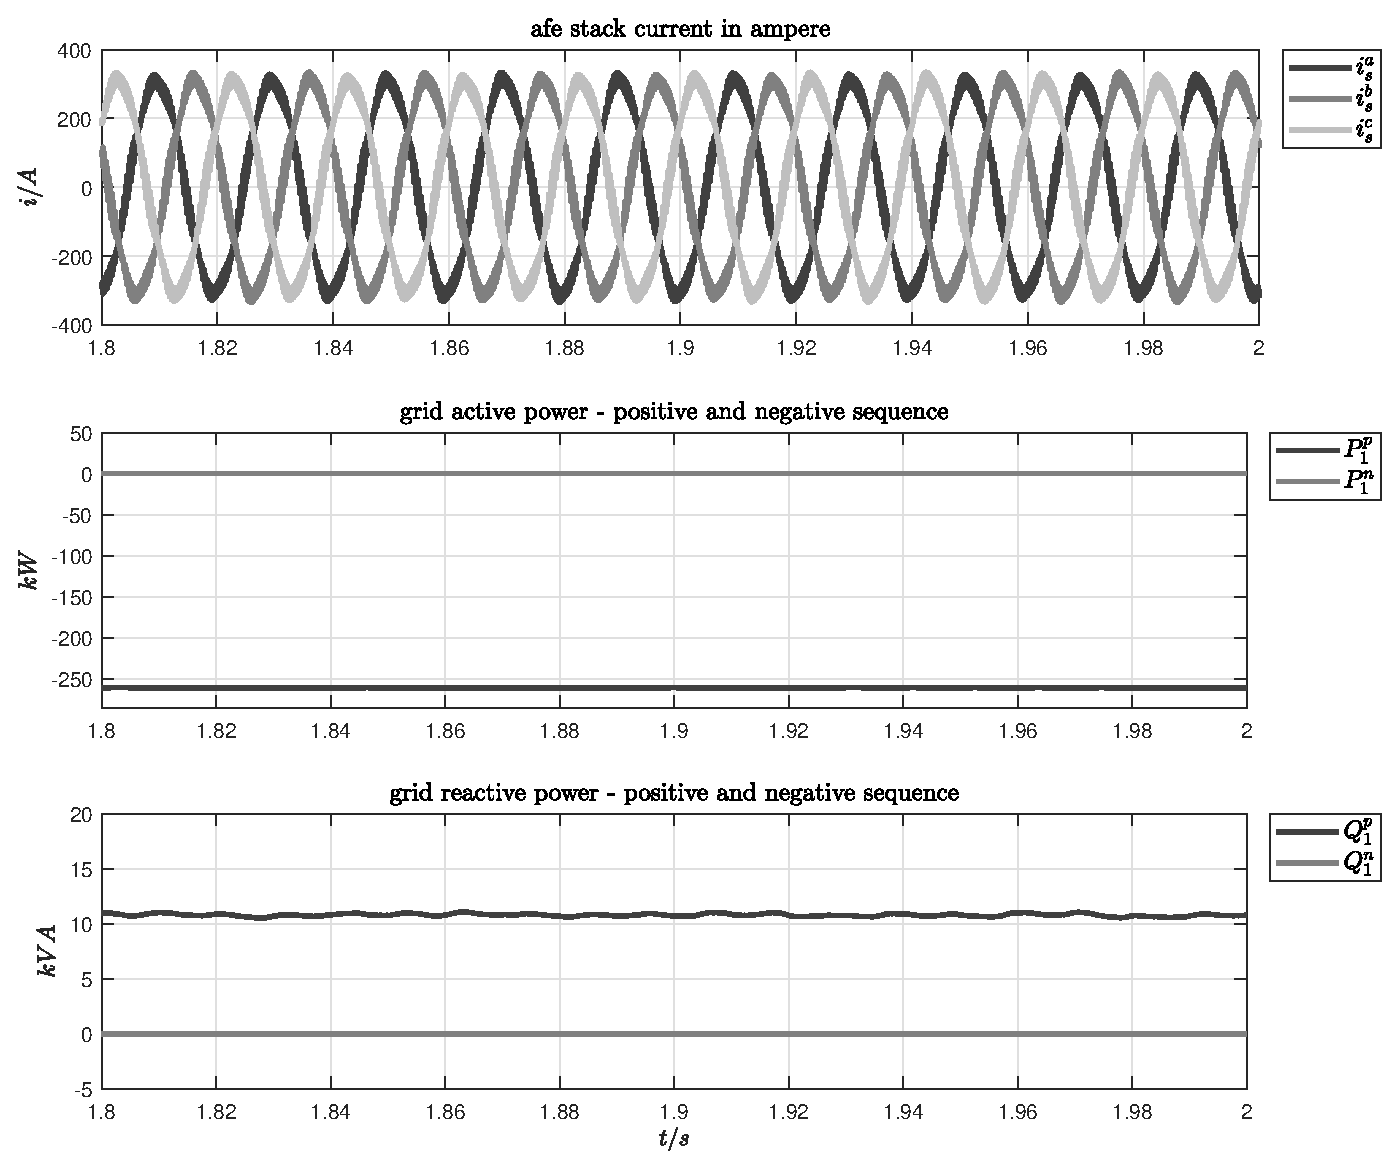
\includegraphics[width =225pt, angle = 0, 
		keepaspectratio]{figures/sim_results/benchmark_case_3/power_sequences.eps}
		\captionsetup{width=0.95\textwidth, font=footnotesize}	
		\caption{afe stack current respect a stationary reference frame in SI (top); active power components in SI (middle); reactive power components in SI (bottom).}
		\label{}
	\end{subfigure}
	\captionsetup{width=0.65\textwidth, font=small}	
	\caption{grid and afe quantities in SI, during nominal power condition for a single \textit{ElectricalDrive} connected to a $i_{cc} = \SI{50}{\kilo\ampere}$ grid with MV/LV transformer with a nominal power of $P_n = \SI{1150}{\kilo{\volt\ampere}}$.}
	\label{}
\end{figure}

\begin{figure}[H]
	\centering
	\begin{subfigure}{0.5\textwidth}
		\centering
		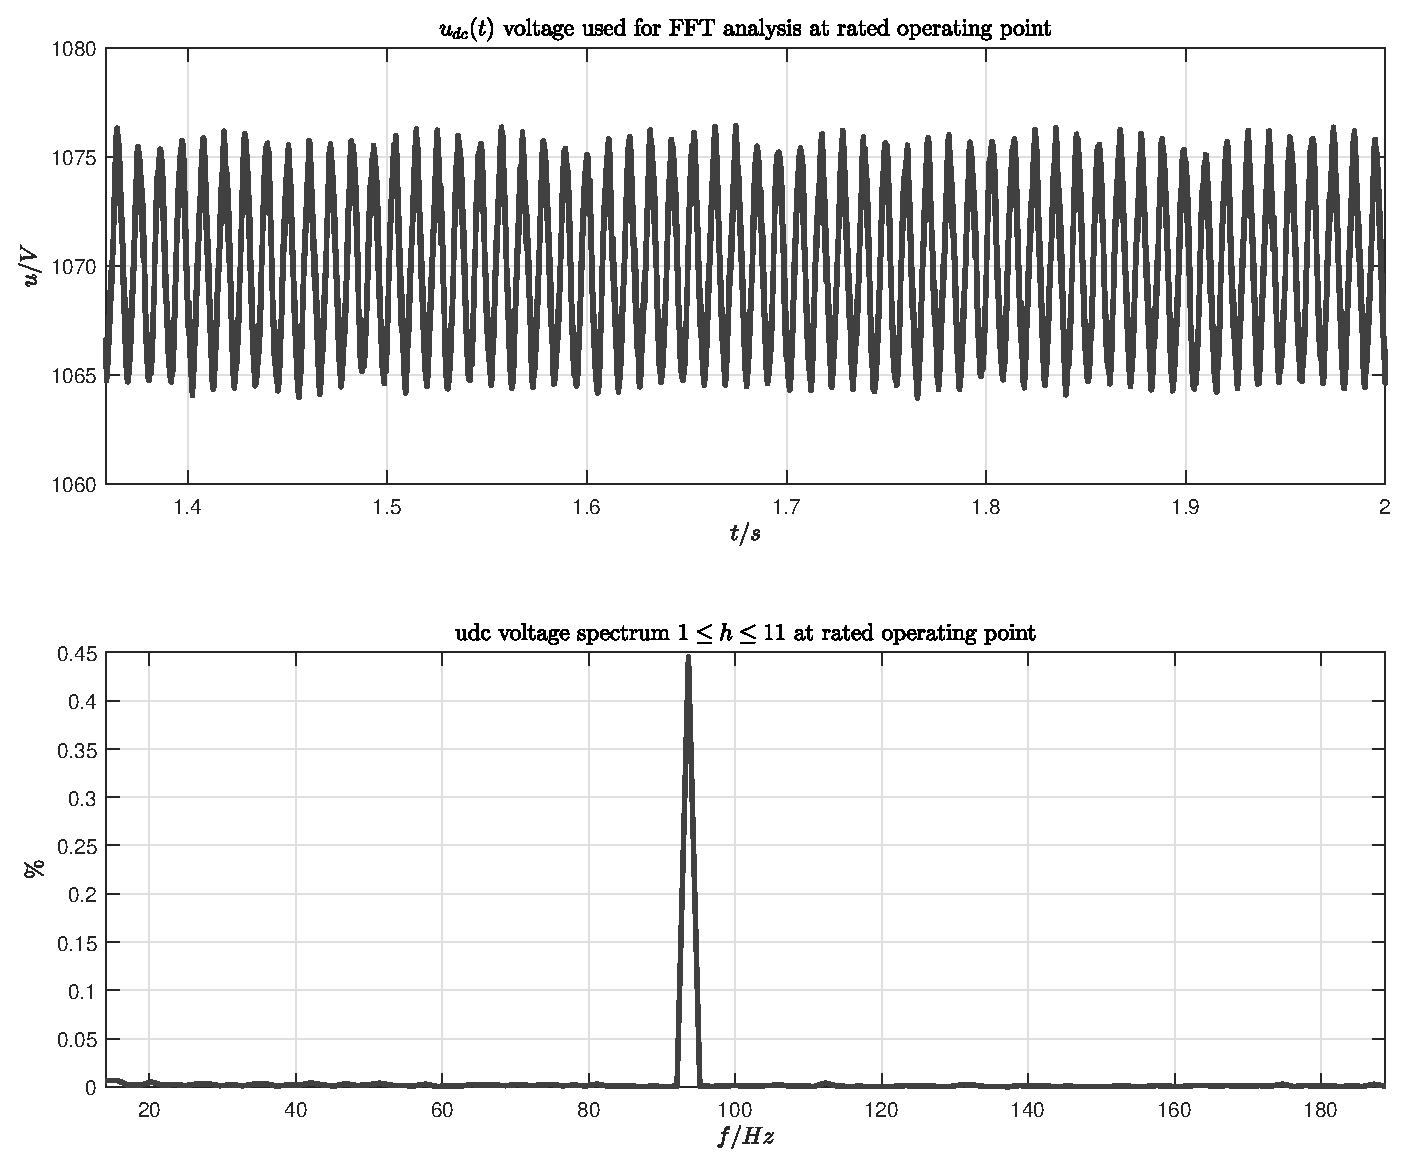
\includegraphics[width =225pt, angle = 0, 
		keepaspectratio]{figures/sim_results/benchmark_case_3/udc_spectrum_figure1.eps}
		\captionsetup{width=0.75\textwidth, font=footnotesize}	
		\caption{DClink voltage, $u_{dc}(t)$, used for spectrum analysis (top); $u_{dc}(t)$ spectrum: relevant is the 6th order component related to the 5th PSM flux component (bottom). $u_{dc}^{base} = \SI{1070}{\volt}$.}
		\label{}
	\end{subfigure}%
	\begin{subfigure}{0.5\textwidth}
		\centering
		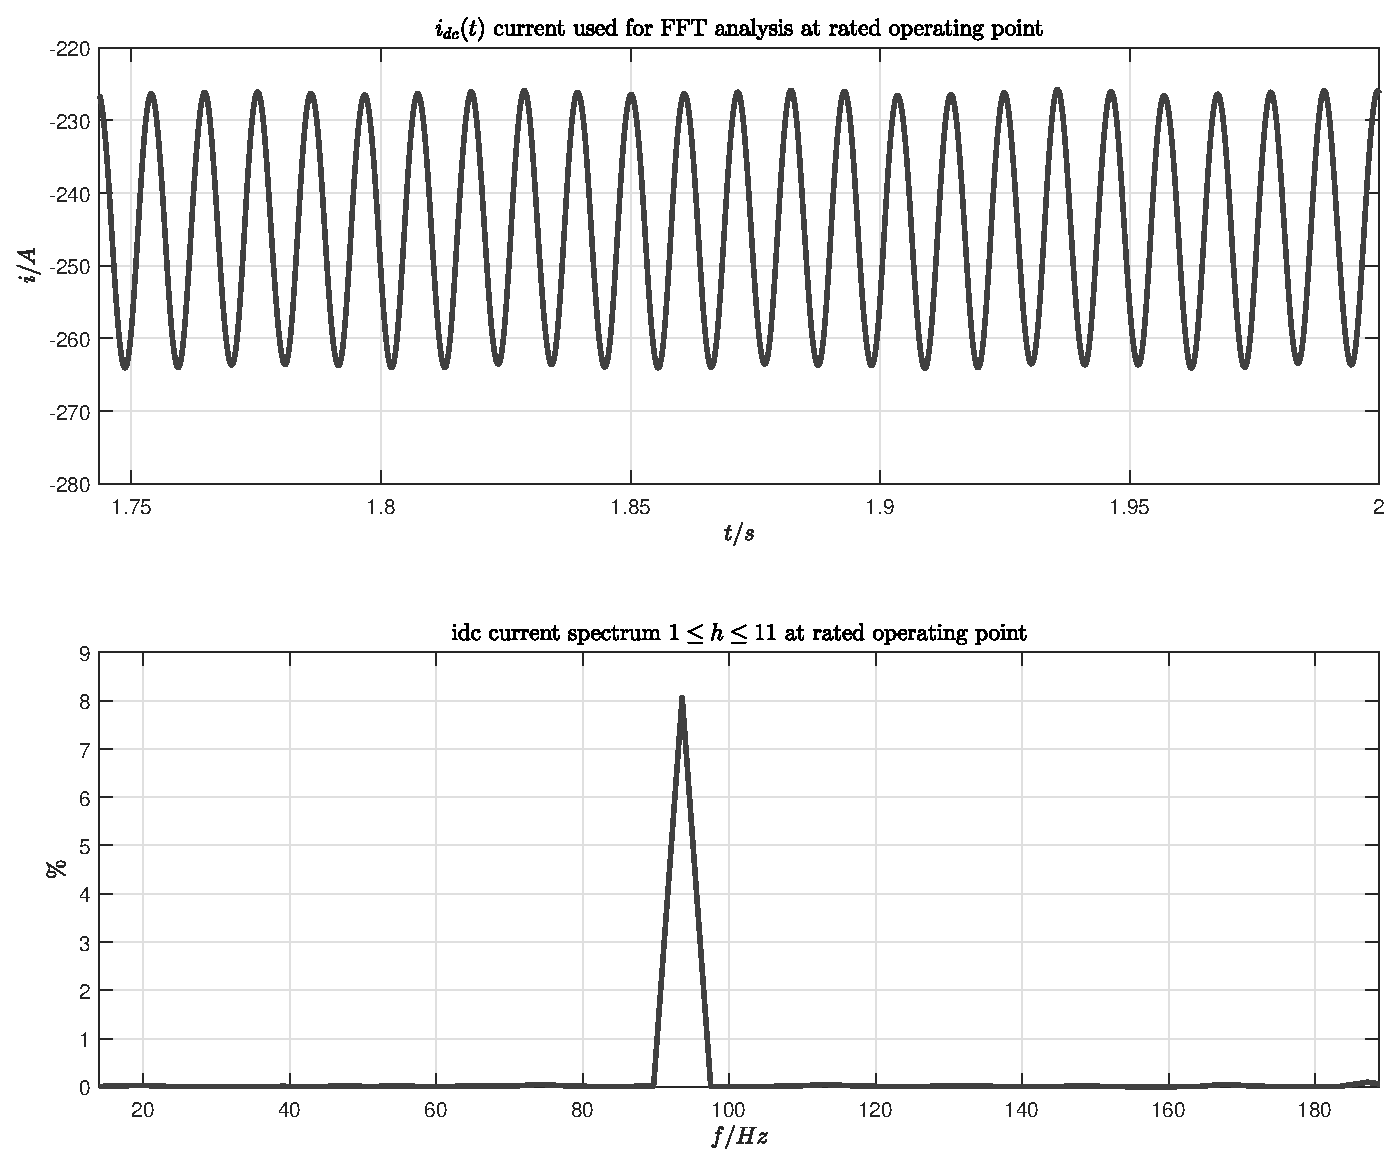
\includegraphics[width =225pt, angle = 0, 
		keepaspectratio]{figures/sim_results/benchmark_case_3/idc_spectrum_figure1.eps}
		\captionsetup{width=0.75\textwidth, font=footnotesize}	
		\caption{DClink current, $i_{dc}(t)$, used for spectrum analysis (top); $i_{dc}(t)$ spectrum: relevant is the 6th order component related to the 5th PSM flux component (bottom). $i_{dc}^{base} = \SI{234}{\ampere}$.}
		\label{}
	\end{subfigure}
	\captionsetup{width=0.65\textwidth, font=small}	
	\caption{DClink quantities in SI, during nominal power condition for a single \textit{ElectricalDrive} connected to a $i_{cc} = \SI{50}{\kilo\ampere}$ grid with MV/LV transformer with a nominal power of $P_n = \SI{1150}{\kilo{\volt\ampere}}$.}
	\label{}
\end{figure}

\subsection{Effects of the grid impedance}
In the following subsection the effects of the grid (line) impedance on grid current harmonic content is investigated. \textbf{Same operating condition will be applied to the same system where the only discrepancy lays into the grid (line) impedance as shown below}.

\begin{itemize}
	\item[--] \textbf{Nominal grid current used for normalization} : $I_{g}^{nom}(t) = \SI{295.8}{\ampere}$;	
	\item[--] \textbf{Nominal grid voltage used for normalization} : $U_{g}^{nom}(t) = \SI{563.4}{\volt}$;	
\end{itemize} 

\begin{figure}[H]
	\centering
	\begin{subfigure}{0.5\textwidth}
		\centering
		\includegraphics[width =225pt, angle = 0, 
		keepaspectratio]{figures/sim_results/benchmark_case_1/igrid_spectrum_figure1.eps}
		\captionsetup{width=0.65\textwidth, font=footnotesize}	
		\caption{grid phase current (top); grid phase current spectrum (bottom); components at $\SI{43.6}{\hertz}$ and $\SI{143.6}{\hertz}$ are coupled to the fifth harmonic component of the PSM back EMF; component at $\SI{250}{\hertz}$ is coupled to the homologous grid voltage harmonic component.}
		\label{}
	\end{subfigure}%
	\begin{subfigure}{0.5\textwidth}
		\centering
		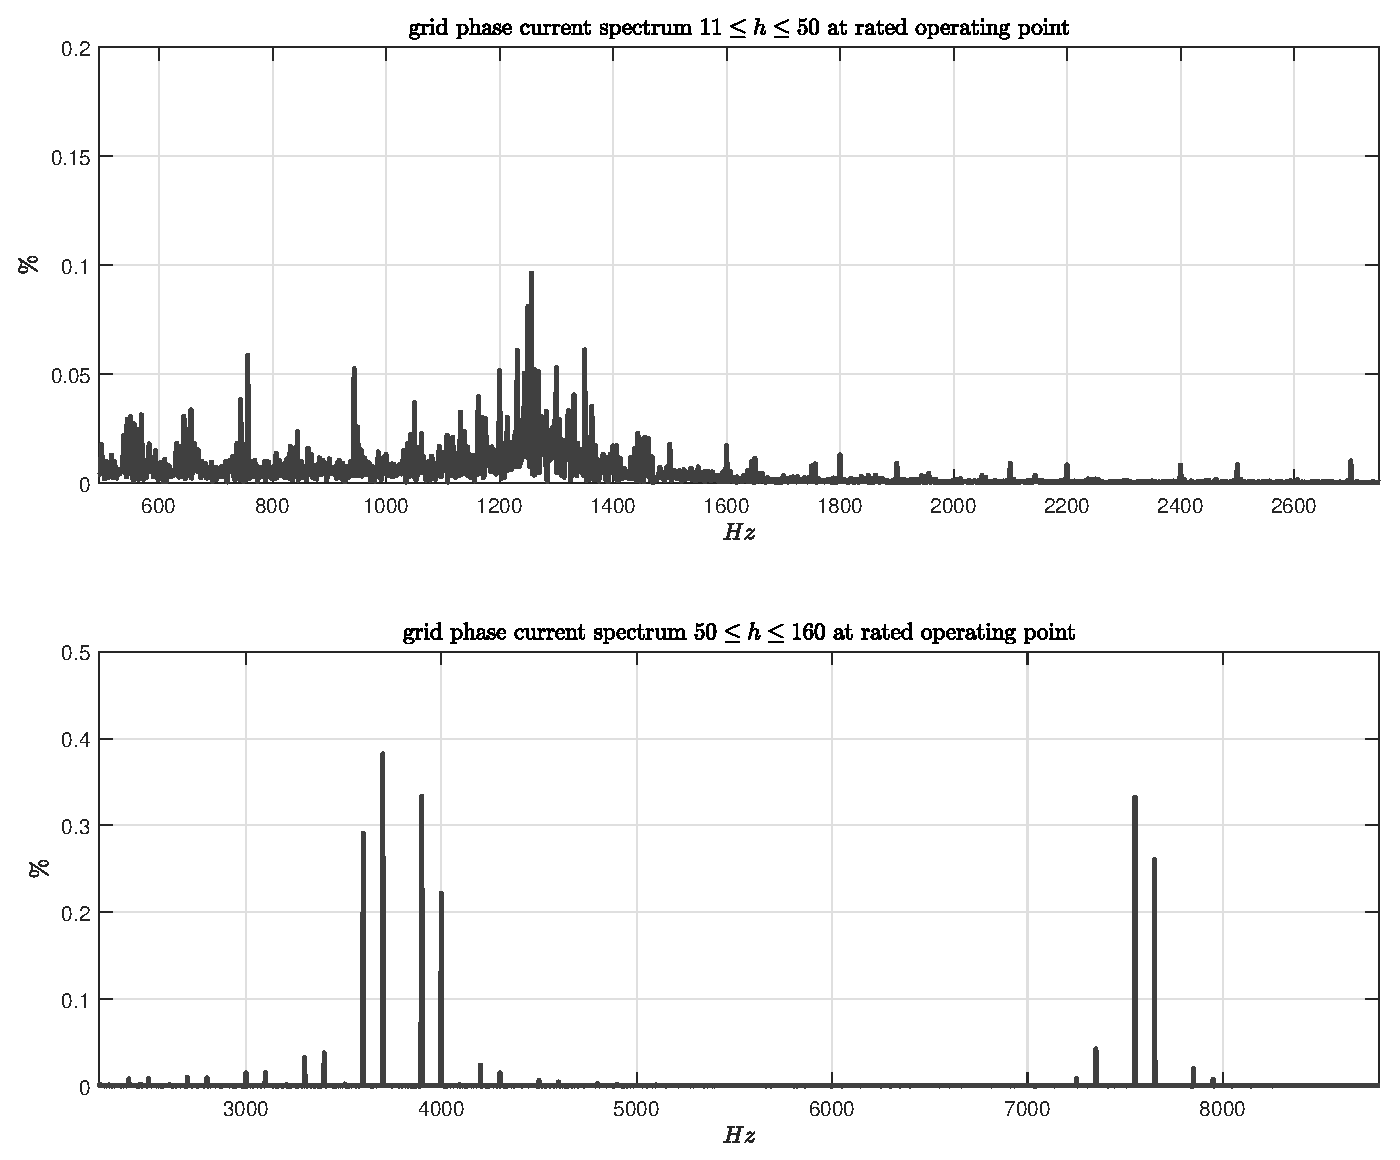
\includegraphics[width =225pt, angle = 0, 
		keepaspectratio]{figures/sim_results/benchmark_case_1/igrid_spectrum_figure2.eps}
		\captionsetup{width=0.75\textwidth, font=footnotesize}	
		\caption{grid current spectrum; effect of the resonance between equivalent grid side inductance ($L_{line} + L_\sigma$) and output filter capacitor of the AFE stage $C_{Fu}$ (top); residual PWM switching harmonic current components (strongly affected by the quantity $L_{line} + L_\sigma$) (bottom).}
		\label{}
	\end{subfigure}
	\captionsetup{width=0.65\textwidth, font=small}	
	\caption{Grid current spectrum for the case of $i_{cc} = \SI{100}{\kilo\ampere}$.}
	\label{}
\end{figure}

\begin{figure}[H]
	\centering
	\begin{subfigure}{0.5\textwidth}
		\centering
		\includegraphics[width =225pt, angle = 0, 
		keepaspectratio]{figures/sim_results/benchmark_case_3/igrid_spectrum_figure1.eps}
		\captionsetup{width=0.65\textwidth, font=footnotesize}	
		\caption{grid phase current (top); grid phase current spectrum (bottom); components at $\SI{43.6}{\hertz}$ and $\SI{143.6}{\hertz}$ are coupled to the fifth harmonic component of the PSM back EMF; component at $\SI{250}{\hertz}$ is coupled to the homologous grid voltage harmonic component.}
		\label{}
	\end{subfigure}%
	\begin{subfigure}{0.5\textwidth}
		\centering
		\includegraphics[width =225pt, angle = 0, 
		keepaspectratio]{figures/sim_results/benchmark_case_3/igrid_spectrum_figure2.eps}
		\captionsetup{width=0.65\textwidth, font=footnotesize}	
		\captionsetup{width=0.75\textwidth, font=footnotesize}	
		\caption{grid current spectrum; effect of the resonance between equivalent grid side inductance ($L_{line} + L_\sigma$) and output filter capacitor of the AFE stage $C_{Fu}$ (top); residual PWM switching harmonic current components (strongly affected by the quantity $L_{line} + L_\sigma$) (bottom).}
		\label{}
	\end{subfigure}
	\captionsetup{width=0.65\textwidth, font=small}	
	\caption{AFE and grid side SI quantities: for the case of $i_{cc} = \SI{50}{\kilo\ampere}$.}
	\label{}
\end{figure}
\begin{figure}[H]
	\centering
	\begin{subfigure}{0.5\textwidth}
		\centering
		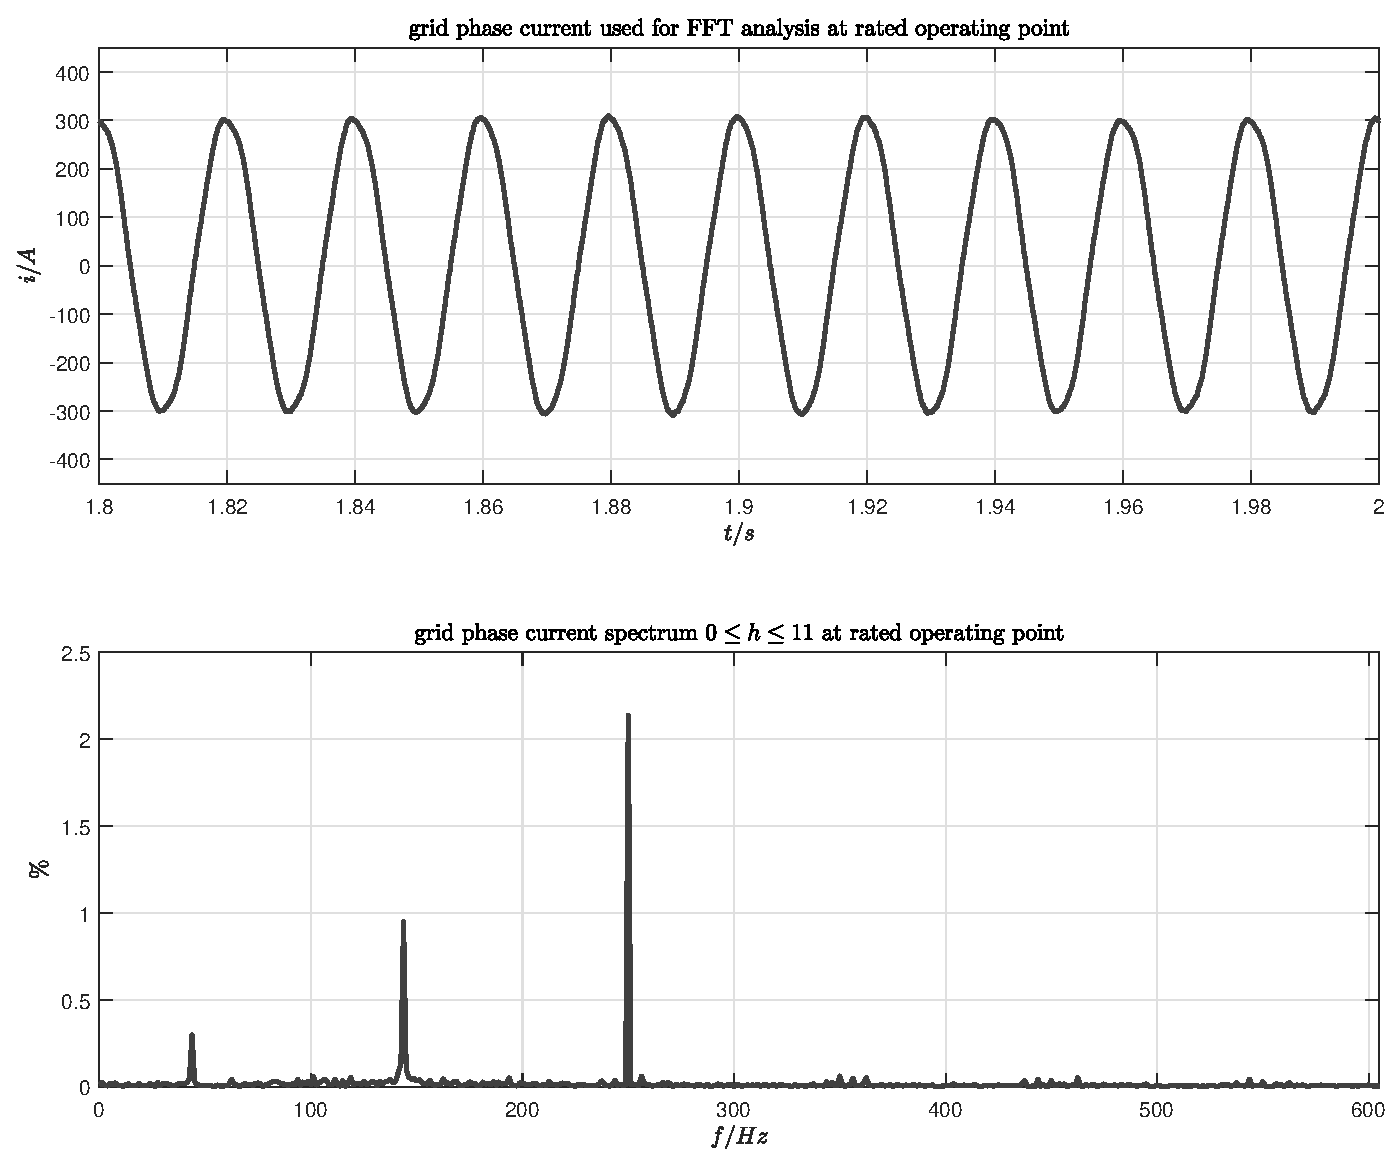
\includegraphics[width =225pt, angle = 0, 
		keepaspectratio]{figures/sim_results/benchmark_case_2/igrid_spectrum_figure1.eps}
		\captionsetup{width=0.65\textwidth, font=footnotesize}	
		\caption{grid phase current (top); grid phase current spectrum (bottom); components at $\SI{43.6}{\hertz}$ and $\SI{143.6}{\hertz}$ are coupled to the fifth harmonic component of the PSM back EMF; component at $\SI{250}{\hertz}$ is coupled to the homologous grid voltage harmonic component.}
		\label{}
	\end{subfigure}%
	\begin{subfigure}{0.5\textwidth}
		\centering
		\includegraphics[width =225pt, angle = 0, 
		keepaspectratio]{figures/sim_results/benchmark_case_2/igrid_spectrum_figure2.eps}
		\captionsetup{width=0.75\textwidth, font=footnotesize}	
		\caption{grid current spectrum; effect of the resonance between equivalent grid side inductance ($L_{line} + L_\sigma$) and output filter capacitor of the AFE stage $C_{Fu}$ (top); residual PWM switching harmonic current components (strongly affected by the quantity $L_{line} + L_\sigma$) (bottom).}
		\label{}
	\end{subfigure}
	\captionsetup{width=0.65\textwidth, font=small}	
	\caption{Grid current spectrum for the case of $i_{cc} = \SI{35}{\kilo\ampere}$.}
	\label{}
\end{figure}

\subsection{Theoretical investigation on one \textit{ElectricalDrive} benchmark simulation results}\label{fifth_harmonic_psm}
Grid current harmonics content is dependent by many factors, as follows
\begin{itemize}
	\item[--] \textbf{pre-existing grid voltage harmonics content};
	\item[--] \textbf{residual PWM switching current};
	\item[--] grid filter residual resonance (as function of grid inductance) components;
	\item[--] distortion introduced by current control loops;	 
	\item[--] \textbf{PSM flux harmonics};	 
\end{itemize} 
Simulation results, already presented in this document, had been made by the use of the above source of distortions, in particular in this sub-section the contribution of the PSM flux distortion will be, in detail, investigated. 

In general in PSM machines, the major contribution of distortion comes from 5th and 7th flux harmonic components which are visible in the back EMF voltage spectrum. In general the 5th harmonic component rotate in negative direction (respect to the fundamental) as well as the 7th harmonic component rotate in positive direction respect to the fundamental. 

Both 5th and 7th harmonic distortions generate a torque ripple which pulses at six times the electrical fundamental pulsation.

Suppose the machine flux can be written as follows, $h_5$ and $h_7$ represent the portion of flux distortion in per unit:
\begin{equation}
	\left\lbrace 
	\begin{aligned}
		\psi_r^u &=\psi^m\sin\left(\vartheta\right) + h_{5}\,\psi^m\sin\left({-5\vartheta}\right) + h_{7}\,\psi^m\sin\left({7\vartheta}\right) \\[6pt]
		\psi_r^v &=\psi^m\sin\left(\vartheta-\frac{{2\pi}}{3}\right) + h_{5}\,\psi^m\sin\left({-5\vartheta-\frac{{2\pi}}{3}}\right) + h_{7}\,\psi^m\sin\left({7\vartheta-\frac{{2\pi}}{3}}\right) \\[6pt]
		\psi_r^w &=\psi^m\sin\left(\vartheta+\frac{{2\pi}}{3}\right) + h_{5}\,\psi^m\sin\left({-5\vartheta+\frac{{2\pi}}{3}}\right) + h_{7}\,\psi^m\sin\left({7\vartheta+\frac{{2\pi}}{3}}\right)
	\end{aligned}
	\right. 
\end{equation}


\begin{equation}
	\left\lbrace 
	\begin{aligned}
			\frac{{d\psi_r^u}}{dt} &=-\omega \Bigg[\psi^m\sin \left( \vartheta \right) - 5\,h_{5}\,\psi^m\sin\left({-5\vartheta}\right) + 7\,h_{7}\,\psi^m\sin\left({7\vartheta}\right) \Bigg] \\[6pt]
		\frac{{d\psi_r^v}}{dt} &= -\omega \Bigg[\psi^m\sin\left(\vartheta - \frac{2\pi}{3}\right) - 5\,h_{5}\,\psi^m\sin\left({-5\vartheta-\frac{{2\pi}}{3}}\right) + 7\,h_{7}\,\psi^m\sin\left({7\vartheta-\frac{{2\pi}}{3}}\right)\Bigg] \\[6pt]
		\frac{{d\psi_r^w}}{dt} &=-\omega \Bigg[\psi^m\sin\left({\vartheta+\frac{{2\pi}}{3}}\right) - 5\,h_{5}\,\psi^m\sin\left({-5\vartheta+\frac{{2\pi}}{3}}\right) + 7\,h_{7}\,\psi^m\sin\left({7\vartheta+\frac{{2\pi}}{3}}\right)\Bigg]
	\end{aligned}
	\right. 
\end{equation}

\begin{equation}\label{uvw_back_emf_1}
	\left\lbrace 
	\begin{aligned}
		e^u(t) & = -E_1\sin\left(\vartheta\right)  + 5\,h_5\,E_1\sin\left(-5\vartheta\right) - 7\,h_7\,E_1\sin\left(7\vartheta\right)\\[6pt]
		e^v(t) & = -E_1\sin\left(\vartheta - \frac{2\pi}{3})\right) + 5\,h_5\,E_1\sin\left(-5\vartheta - \frac{2\pi}{3}\right) - 7\,h_7\,E_1\sin\left(7\vartheta - \frac{2\pi}{3}\right)\\[6pt]
		e^w(t) & = -E_1\sin\left(\vartheta + \frac{2\pi}{3})\right) + 5\,h_5\,E_1\sin\left(-5\vartheta + \frac{2\pi}{3}\right) - 7\,h_7\,E_1\sin\left(7\vartheta + \frac{2\pi}{3}\right)
	\end{aligned}
	\right. 
\end{equation}
In a 3-wire three phase system Kirchhoff condition $x_a+x_b+x_c=0$ holds, that means the phase vector lays in a plane (2-dimensions), and that means the whole three phase system can be 
written by the use of two components $(\alpha,\beta)$, applying the coordinates transformation $\mathbf{T}_1$ defined as follows:
\begin{equation}
	\begin{aligned}
		\mathbf{T}_1 = 
		\frac{2}{3}\begin{bmatrix}
			1 & -\frac{1}{2} & -\frac{1}{2} \\[6pt]
			0 & \frac{\sqrt{3}}{2} & -\frac{\sqrt{3}}{2} 
		\end{bmatrix} \qquad
		\mathbf{T}_1^{-1} = 
		\begin{bmatrix}
			1 & 0 \\[6pt]
			-\frac{1}{2} & \frac{\sqrt{3}}{2} \\[6pt]
			-\frac{1}{2} & -\frac{\sqrt{3}}{2} 
		\end{bmatrix}
	\end{aligned} 
\end{equation}
\begin{equation}
	\mathbf{T}_1\mathbf{T}_1^{-1} = \mathbf{I}_2
\end{equation}
where 
\begin{equation}\label{t1}
	\begin{aligned}
		\vec{x}_{\alpha\beta}=\mathbf{T}_1\vec{x}_{uvw}
	\end{aligned} 
\end{equation}

Applying \eqref{t1} to \eqref{uvw_back_emf_1} it results
\begin{equation}\label{alphabeta_back_emf_1}
	\left\lbrace 
	\begin{aligned}
		e^{\alpha}(t) & = -E_1\sin\left(\vartheta\right)  - 5\,h_5\,E_1\sin\left(-5\vartheta\right) + 7\,h_7\,E_1\sin\left(7\vartheta \right) \\[6pt]
		e^{\beta}(t) & = E_1\cos\left(\vartheta\right) - 5\,h_5\,E_1\cos\left(-5\vartheta\right) + 7\,h_7\,E_1\cos\left(7\vartheta\right)
	\end{aligned}
	\right. 
\end{equation}
changing reference frame from stationary to synchronous\footnote{
\begin{multicols}{2}
	\begin{figure}[H]
		\centering
		\includegraphics[width = 225pt, 
		keepaspectratio]{figures/psm/reference_frames_dq_ii.eps}
		\captionsetup{width=0.5\textwidth, font=small} \caption	{Reference frames}
		\label{dq_ref_frame}
	\end{figure}
	\begin{align}\label{t2}
			\vec{x}_{dq}=\mathbf{T}_2\vec{x}_{\alpha\beta} &&
	\end{align}
	\begin{align}\label{t2_1}
			\mathbf{T}_2^{-1}\vec{x}_{dq}=\vec{x}_{\alpha\beta} &&
	\end{align}
	where
	\begin{align}
			\mathbf{T}_2(\vartheta_0) = 
			\begin{bmatrix}
				\cos(\vartheta_0) & \sin(\vartheta_0) \\[6pt]
				-\sin(\vartheta_0) & \cos(\vartheta_0) 
			\end{bmatrix} &&
	\end{align}
	\begin{align}
			\mathbf{T}_2^{-1}(\vartheta_0) = 
			\begin{bmatrix}
				\cos(\vartheta_0) & -\sin(\vartheta_0) \\[6pt]
				\sin(\vartheta_0) & \cos(\vartheta_0) 
			\end{bmatrix} &&
	\end{align}
	\begin{align}
			\mathbf{T}_2(\vartheta_0) \ \mathbf{T}_2^{-1}(\vartheta_0) = \mathbf{I}_2 &&
	\end{align}
\end{multicols}
}
\eqref{alphabeta_back_emf_1} become
\begin{equation}\label{dq_back_emf_1}
	\left\lbrace 
	\begin{aligned}
		e^{d}(t) & = -5\,h_5\,E_1\sin\left( -6\vartheta \right) + 7\,h_7\,E_1\sin\left(6\vartheta \right)\\[6pt]
		e^{q}(t) & = E_1 - 5\,h_5\,E_1\cos\left(-6\vartheta\right) - 7\,h_7\,E_1\cos\left(6\vartheta\right)
	\end{aligned}
	\right. 
\end{equation}
if $5\,h_5\approx7\,h_7$ (a condition which can be reasonably satisfied) \eqref{dq_back_emf_1} become
\begin{equation}\label{dq_back_emf_2}
	\left\lbrace 
	\begin{aligned}
		e^{d}(t) & \approx 0 \\[6pt]
		e^{q}(t) & = E_1 - E_6 \cos\left(6\vartheta\right)
	\end{aligned}
	\right. 
\end{equation}
where $e^{d}(t)$ and $e^{q}(t)$ represent the back EMF voltage of the PSM.

Supposing a perfect sinusoidal PSM current, the total power flowing through the DClink can be represented as follow
\begin{equation}
		\begin{aligned}
	p(t) &= e^{d}(t)\,i_d(t) + e^{q}(t)\,i_q(t) = \\[6pt]
		 &= p_1(t) + p_6(t)
		\end{aligned}
\end{equation}
where total power is composed by two terms
\begin{itemize}
	\item[--] $p_1(t)$ : constant instantaneous active power which reflects the quantity $\omega_m(t)\tau_e(t)$;  
	\item[--] $p_6(t)$ : pulsating instantaneous active power due to the torque ripple\footnote{generating sound emission and residual grid current harmonics};  
\end{itemize}

Part of the term $p_6(t) = P_{h6}\cos(6\vartheta)$ will be injected into the grid in the form of current harmonic components as follows
\begin{itemize}
	\item[--] let $i_\xi(t) = i_1^\xi(t) + i_6^\xi(t)\cos(6\vartheta)$ the instantaneous active grid current, where 
	\begin{equation}
		\frac{d\vartheta}{dt} = \omega
	\end{equation} is PSM electrical pulsation;  
	\item[--] the equivalent \textit{abc} grid current are generated by the transformation 
	\begin{equation}
		\begin{aligned}
			& \mathbf{T}_2(\vartheta_g) = 
			\begin{bmatrix}
				\cos(\vartheta_g) & \sin(\vartheta_g) \\[6pt]
				-\sin(\vartheta_g) & \cos(\vartheta_g) 
			\end{bmatrix} \quad
			& \mathbf{T}_2^{-1}(\vartheta_g) = 
			\begin{bmatrix}
				\cos(\vartheta_g) & -\sin(\vartheta_g) \\[6pt]
				\sin(\vartheta_g) & \cos(\vartheta_g) 
			\end{bmatrix} \quad
			& \mathbf{T}_2(\vartheta_g) \ \mathbf{T}_2^{-1}(\vartheta_g)= \mathbf{I}_2
		\end{aligned} 
		\end{equation} where \begin{equation}\frac{d\vartheta_g}{dt} = \omega_g\end{equation} is grid electrical pulsation;  
\end{itemize}
That means
\begin{equation}
	\begin{bmatrix}
		\cos(\vartheta_g) & -\sin(\vartheta_g) \\[6pt]
		\sin(\vartheta_g) & \cos(\vartheta_g) 
	\end{bmatrix}
	\begin{bmatrix}
		i_\xi(t) \\[6pt]
		0 
	\end{bmatrix} = 
	\begin{bmatrix}
		i_1^\xi(t)\cos(\vartheta_g) + i_6^\xi(t)\cos(6\vartheta)\cos(\vartheta_g) \\[6pt]
		i_1^\xi(t)\sin(\vartheta_g) + i_6^\xi(t)\cos(6\vartheta)\sin(\vartheta_g)
	\end{bmatrix}
\end{equation}
the term $i_6^\xi(t)\cos(6\vartheta)\cos(\vartheta_g)$ can be decomposed into 
\begin{equation}
	\begin{aligned}
		i_6^\xi(t)\cos(6\vartheta)\cos(\vartheta_g) = \frac{i_6^\xi(t)}{2}\Big[\cos(\vartheta_g+6\vartheta)+\cos(\vartheta_g-6\vartheta)\Big]
	\end{aligned}
\end{equation}
as well as the term $i_6^\xi(t)\cos(6\vartheta)\sin(\vartheta_g)$ can be decomposed into 
\begin{equation}
	\begin{aligned}
		i_6^\xi(t)\cos(6\vartheta)\sin(\vartheta_g) = \frac{i_6^\xi(t)}{2}\Big[\sin(\vartheta_g+6\vartheta)+\sin(\vartheta_g-6\vartheta)\Big]
	\end{aligned}
\end{equation}
\noindent\textbf{Remark} - the presence of negative rotating 5th PSM flux harmonic component (positive rotating 7th PSM flux harmonic component) generates an active power component pulsating at 6th order, of the fundamental PSM pulsation, at the DClink power stage. The 6th order pulsation at the DClink stage ($6\vartheta$) will appear at the grid side (three phase system pulsating at $\omega_g$) with the components $\vartheta_g - 6\vartheta$ and $\vartheta_g + 6\vartheta$ where $\vartheta_g$ is the electrical grid phase while $\vartheta$ is the electrical PSM phase.

\section{Case scenario analysis}	
In this section overall case scenario, concerning the \textit{ElectricalDrive} configuration will be investigated. Below a list of all cases is shown:
\begin{myitemize_2}
	\item[--] \textbf{case scenario 1} - $P_n = \SI{1150}{\kilo{\volt\ampere}}$  - four \textit{ElectricalDrive} connected to four, galvanically isolated PSM three phase system, as per Figure~\ref{ElectricalDrive_connection_figure_1b};
	\item[--] \textbf{case scenario 2} - $P_n = \SI{1670}{\kilo{\volt\ampere}}$  - two, galvanically isolated PSM three phase system, connected, each one, to three hard-parallelized \textit{ElectricalDrive}, as per Figure~\ref{ElectricalDrive_connection_figure_2b};
	\item[--] \textbf{case scenario 3} - $2\ \times \ P_n = \SI{1150}{\kilo{\volt\ampere}}$  - two power system connected to the same PCC which each one consists of four \textit{ElectricalDrive} connected to four, galvanically isolated PSM three phase system, as per Figure~\ref{ElectricalDrive_connection_figure_3b};
	\item[--] \textbf{case scenario 4} - $\ P_n = \SI{1850}{\kilo{\volt\ampere}}$  - eight \textit{ElectricalDrive} connected to eight, galvanically isolated PSM three phase system, as per Figure~\ref{ElectricalDrive_connection_figure_6};
\end{myitemize_2}

\subsection{Case scenario 1 - four galvanically isolated systems ($\mathbf{P_{plant} = \SI{1150}{\kilo{\volt\ampere}}}$)}	
This subsection shows the simulation results for the following case scenario
\begin{itemize}
	\item[--] the PSM generator is made by four galvanically isolated three phase systems;
	\item[--] all four PSM three phase systems have the same back EMF waveform in terms of fundamental amplitude, phase, and harmonic distortion (in other words all systems are overlapped);
	\item[--] each PSM three phase system is connected to the grid by a modular electrical drive (\textit{ElectricalDrive}); 
	\item[--] all \textit{ElectricalDrive} are connected to the grid via a Dyn11 MV/LV transformer with a nominal power of $P_n=\SI{1150}{\kilo{\volt\ampere}}$ and $u_{cc} = \SI{6}{\percent}$\footnote{The relation between $u_{cc}$ and residual leakage inductance is given by the formula
	\begin{align}
		L_\sigma &= u_{cc}\frac{U_2}{\sqrt{3}\,I_2\,\omega} &&
	\end{align}
	where $I_2 = \frac{P_n}{\sqrt{3}\,U_2}$
};
	\item[--] line inductance is assumed equal to $L_{line} = \SI{25.4}{\micro\henry}$ which corresponds to a prospective short circuit current at PCC of $i_{cc} = \SI{50}{\kilo\ampere}$ (\textbf{remark}: equivalent values seen at LV side);	
	\item[--] all space vector modulators (four for AFE and four for INVERTER) are synchronized and \textit{in phase}; \textbf{remark}: this correspond to a worst case scenario;
\end{itemize}

\begin{figure}[H]
	\centering
	\includegraphics[width = 500pt, angle = 0, 
	keepaspectratio]{figures/ElectricalDrive_connection_figure_1b.eps}
	\captionsetup{width=0.75\textwidth, font=small}	
	\caption{Functional representation of the 1MW power solution. The configuration is made by four \textit{ElectricalDrive} each one connected, at inverter side, to one, galvanically isolated PSM three phase system; at grid side the \textit{ElectricalDrive} are connected to each other to create a common connection point.}
	\label{ElectricalDrive_connection_figure_1b}
\end{figure}

\begin{figure}[H]
	\centering
	\begin{subfigure}{0.5\textwidth}
		\centering
		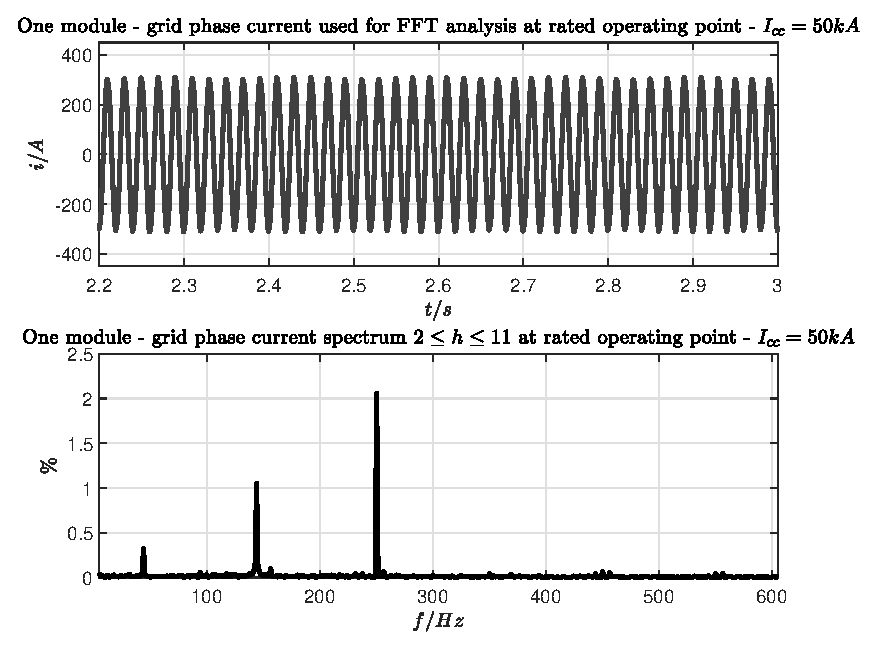
\includegraphics[width =225pt, angle = 0, 
		keepaspectratio]{figures/sim_results/case_1x1150kVA/igrid_1mod_spectrum_figure1.eps}
		\captionsetup{width=0.95\textwidth, font=footnotesize}	
		\caption{Grid current waveform $i_{line} = n\cdot i_{g}$ with $n=1$ (top), and spectrum analysis of the grid current (bottom). The components related to the 5th PSM harmonic distortion are visible at frequency of $\SI{43.6}{\hertz}$, and $\SI{143.6}{\hertz}$, while the residual current harmonic distortion correlated to the 5th harmonic grid voltage is visible at frequency of $\SI{250.0}{\hertz}$.}
		\label{}
	\end{subfigure}%
	\begin{subfigure}{0.5\textwidth}
		\centering
		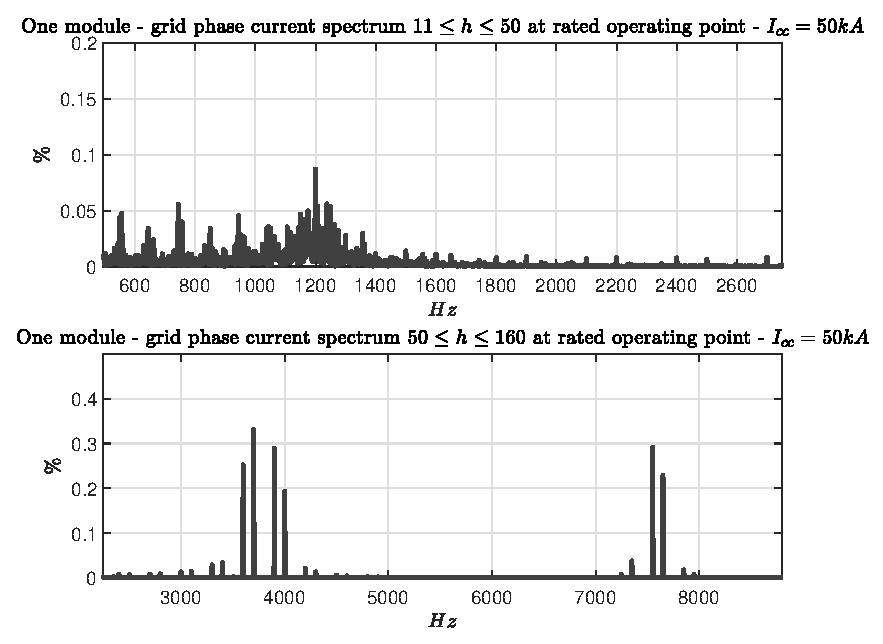
\includegraphics[width =225pt, angle = 0, 
		keepaspectratio]{figures/sim_results/case_1x1150kVA/igrid_1mod_spectrum_figure2.eps}
		\captionsetup{width=0.75\textwidth, font=footnotesize}	
		\caption{Grid current spectrum analysis: grid filter resonance effect is visible (top) around the frequency $f_0=\frac{1}{2\pi\sqrt{L_{grid}\cdot n \cdot C_{Fu}}}$, where $L_{grid} = L_{line} + L_{\sigma}$; residual grid current harmonics related to the PWM modulation are also visible (bottom).}
		\label{}
	\end{subfigure}
	\captionsetup{width=0.65\textwidth, font=small}	
	\caption{Case study with one \textit{ElectricalDrive} operating at 250kW. Current base used for normalization is $i_{line}^{base}\Big|_{m1}=\sqrt{\frac{2}{3}}\frac{P_{base}}{u_{nom}}=\SI{295.8}{\ampere}$, where $P_{base}=\SI{250}{\kilo\watt}$, and $u_{nom}=\SI{690}{\volt}$; the total residual current distortion is $\textit{THD}_i = \SI{2.46}{\percent}$.}
	\label{}
\end{figure}

\begin{figure}[H]
	\centering
	\begin{subfigure}{0.5\textwidth}
		\centering
		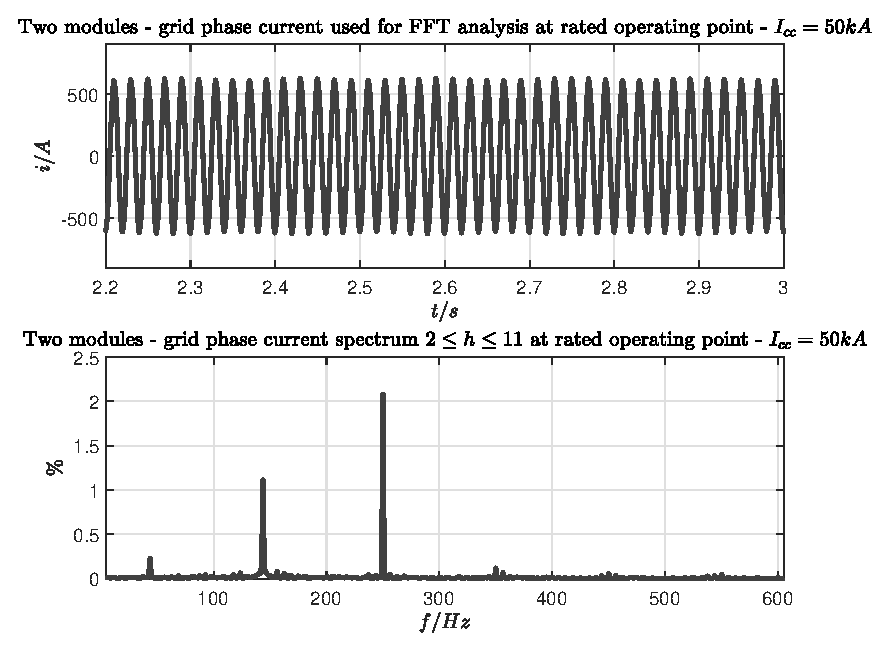
\includegraphics[width =225pt, angle = 0, 
		keepaspectratio]{figures/sim_results/case_1x1150kVA/igrid_2mods_spectrum_figure1.eps}
		\captionsetup{width=0.95\textwidth, font=footnotesize}	
		\caption{Grid current waveform $i_{line} = n\cdot i_{g}$, with $n=2$ (top), and spectrum analysis of the grid current (bottom). The components related to the 5th PSM harmonic distortion are visible at frequency of $\SI{43.6}{\hertz}$, and $\SI{143.6}{\hertz}$, while the residual current harmonic distortion correlated to the 5th harmonic grid voltage is visible at frequency of $\SI{250.0}{\hertz}$.}
		\label{}
	\end{subfigure}%
	\begin{subfigure}{0.5\textwidth}
		\centering
		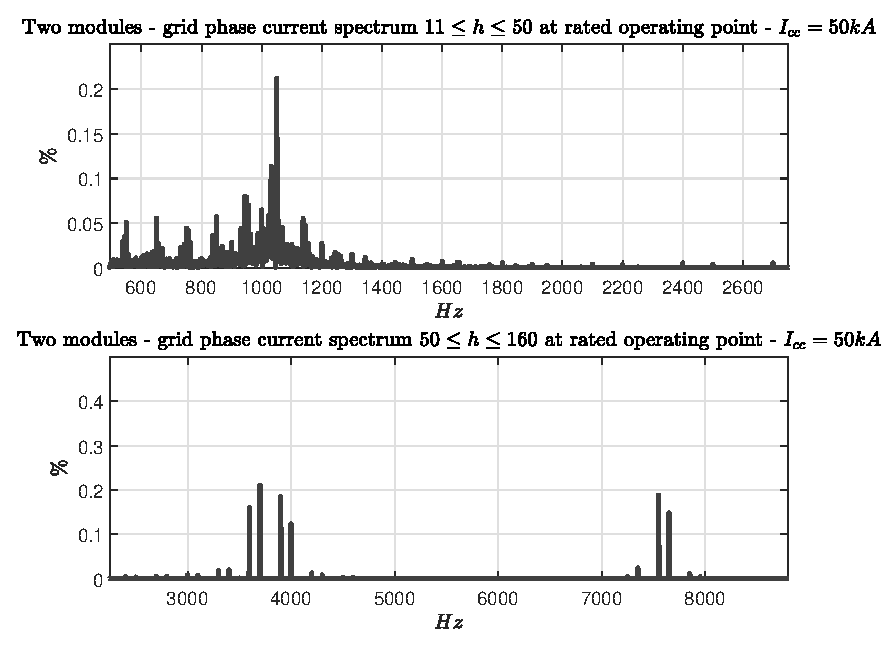
\includegraphics[width =225pt, angle = 0, 
		keepaspectratio]{figures/sim_results/case_1x1150kVA/igrid_2mods_spectrum_figure2.eps}
		\captionsetup{width=0.75\textwidth, font=footnotesize}	
		\caption{Grid current spectrum analysis: effects of the resonance are visible (top) around the frequency $f_0=\frac{1}{2\pi\sqrt{L_{grid}\cdot n \cdot C_{Fu}}}$, where $L_{grid} = L_{line} + L_{\sigma}$; residual grid current harmonics related to the PWM modulation are also visible (bottom).}
		\label{}
	\end{subfigure}
	\captionsetup{width=0.65\textwidth, font=small}	
	\caption{Case study with two \textit{ElectricalDrive} each one operating at 250kW. Current base used for normalization is $i_{line}^{base}\Big|_{m2}=\sqrt{\frac{2}{3}}\frac{P_{base}}{u_{nom}}=\SI{591.7}{\ampere}$, where $P_{base}=\SI{500}{\kilo\watt}$, and $u_{nom}=\SI{690}{\volt}$; the total residual current distortion is $\textit{THD}_i = \SI{2.25}{\percent}$.}
	\label{}
\end{figure}

\begin{figure}[H]
	\centering
	\begin{subfigure}{0.5\textwidth}
		\centering
		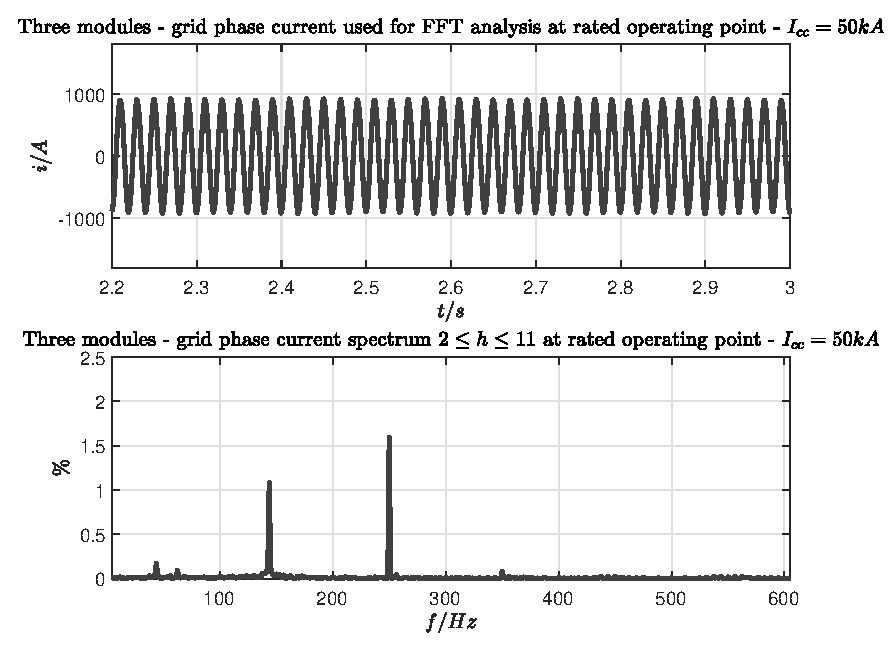
\includegraphics[width =225pt, angle = 0, 
		keepaspectratio]{figures/sim_results/case_1x1150kVA/igrid_3mods_spectrum_figure1.eps}
		\captionsetup{width=0.95\textwidth, font=footnotesize}	
		\caption{Grid current waveform $i_{line} = n\cdot i_{g}$, with $n=3$ (top), and spectrum analysis of the grid current (bottom). The components related to the 5th PSM harmonic distortion are visible at frequency of $\SI{43.6}{\hertz}$, and $\SI{143.6}{\hertz}$, while the residual current harmonic distortion correlated to the 5th harmonic grid voltage is visible at frequency of $\SI{250.0}{\hertz}$.}
		\label{}
	\end{subfigure}%
	\begin{subfigure}{0.5\textwidth}
		\centering
		\includegraphics[width =225pt, angle = 0, 
		keepaspectratio]{figures/sim_results/case_1x1150kVA/igrid_3mods_spectrum_figure2.eps}
		\captionsetup{width=0.75\textwidth, font=footnotesize}	
		\caption{Grid current spectrum analysis; effects of the resonance are visible (top) around the frequency $f_0=\frac{1}{2\pi\sqrt{L_{grid}\cdot n \cdot C_{Fu}}}$, where $L_{grid} = L_{line} + L_{\sigma}$; residual grid current harmonics related to the PWM modulation are also visible (bottom).}
		\label{}
	\end{subfigure}
	\captionsetup{width=0.65\textwidth, font=small}	
	\caption{Case study with three \textit{ElectricalDrive} each one operating at 250kW. Current base used for normalization is $i_{line}^{base}\Big|_{m3}=\sqrt{\frac{2}{3}}\frac{P_{base}}{u_{nom}}=\SI{887.5}{\ampere}$, where $P_{base}=\SI{750}{\kilo\watt}$, and $u_{nom}=\SI{690}{\volt}$; the total residual current distortion is $\textit{THD}_i = \SI{2.0}{\percent}$.}
	\label{}
\end{figure}

\begin{figure}[H]
	\centering
	\begin{subfigure}{0.5\textwidth}
		\centering
		\includegraphics[width =225pt, angle = 0, 
		keepaspectratio]{figures/sim_results/case_1x1150kVA/igrid_4mods_spectrum_figure1.eps}
		\captionsetup{width=0.95\textwidth, font=footnotesize}	
		\caption{Grid current waveform $i_{line} = n\cdot i_{g}$, with $n=4$ (top), and spectrum analysis of the grid current (bottom). The components related to the 5th PSM harmonic distortion are visible at frequency of $\SI{43.6}{\hertz}$, and $\SI{143.6}{\hertz}$, while the residual current harmonic distortion correlated to the 5th harmonic grid voltage is visible at frequency of $\SI{250.0}{\hertz}$.}
		\label{}
	\end{subfigure}%
	\begin{subfigure}{0.5\textwidth}
		\centering
		\includegraphics[width =225pt, angle = 0, 
		keepaspectratio]{figures/sim_results/case_1x1150kVA/igrid_4mods_spectrum_figure2.eps}
		\captionsetup{width=0.75\textwidth, font=footnotesize}	
		\caption{Grid current spectrum analysis; effects of the resonance are visible (top) around the frequency $f_0=\frac{1}{2\pi\sqrt{L_{grid}\cdot n \cdot C_{Fu}}}$, where $L_{grid} = L_{line} + L_{\sigma}$; residual grid current harmonics related to the PWM modulation are also visible (bottom).}
		\label{}
	\end{subfigure}
	\captionsetup{width=0.65\textwidth, font=small}	
	\caption{Case study with four \textit{ElectricalDrive} each one operating at 250kW. Current base used for normalization is $i_{line}^{base}\Big|_{m4}=\sqrt{\frac{2}{3}}\frac{P_{base}}{u_{nom}}=\SI{1183.3}{\ampere}$, where $P_{base}=\SI{1000}{\kilo\watt}$, and $u_{nom}=\SI{690}{\volt}$; the total residual current distortion is $\textit{THD}_i = \SI{1.88}{\percent}$.}
	\label{}
\end{figure}

\subsection{Case scenario 2 - two galvanically isolated systems ($\mathbf{P_{plant} = \SI{1500}{\kilo{\volt\ampere}}}$)}	
This subsection shows the simulation results for the following case scenario
\begin{itemize}
	\item[--] the PSM generator is made by two galvanically isolated three phase systems; that means each independent three phase system has a nominal power of 750kW and should be supplied by the hard parallelization of three \textit{ElectricalDrive};
	\item[--] all two PSM three phase systems have the same back EMF waveform in terms of fundamental phase (system are overlapped) as well as harmonic distortion;
	\item[--] each three phase system is connected to the grid by a triplet hard parallelized (\textit{ElectricalDrive}); all \textit{ElectricalDrive} are connected to the grid via a Dyn11 MV/LV transformer with a nominal power of $P_n=\SI{1670}{\kilo{\volt\ampere}}$ and $u_{cc} = \SI{6}{\percent}$;
	\item[--] line inductance is assumed equal to $L_{line} = \SI{25.4}{\micro\henry}$ which corresponds to a prospective short circuit current at PCC of $i_{cc} = \SI{50}{\kilo\ampere}$ (\textbf{remark}: equivalent values seen at LV side);	
	\item[--] all space vector modulators (four for AFE and four for INVERTER) are synchronized and \textit{in phase}; \textbf{remark}: this correspond to a worst case scenario;
\end{itemize}

\begin{figure}[H]
	\centering
	\includegraphics[width = 450pt, angle = 0, 
	keepaspectratio]{figures/ElectricalDrive_connection_figure_2b.eps}
	\captionsetup{width=0.85\textwidth, font=small}	
	\caption{Functional representation of the 1.5MW power solution. The configuration is made by two identical power systems connected each one to a grid common point. Each power system is composed by three hard-parallelized \textit{ElectricalDrive}. The common point at inverter side is therefore connected to a galvanically isolated PSM three phase system. The configuration made by the hard-parallelization of three \textit{ElectricalDrive} is permitted due to the fact that each \textit{ElectricalDrive} is equipped with three-phase inductors which have both differential and common mode inductance. Moreover PWM modulators, belong to the same hard-parallelized circuit, are each other synchronized respect to a master time. An additional zero sequence current control is moreover activated. In case of PWM misalignment a given zero sequence current will flow only among the thee hard-parallelized \textit{ElectricalDrive} and the \textit{line} current will be not affected.}
	\label{ElectricalDrive_connection_figure_2b}
\end{figure}

\begin{figure}[H]
	\centering
	\begin{subfigure}{0.5\textwidth}
		\centering
		\includegraphics[width =225pt, angle = 0, 
		keepaspectratio]{figures/sim_results/case_1x1670kVA/igrid_1mod_spectrum_figure1.eps}
		\captionsetup{width=0.95\textwidth, font=footnotesize}	
		\caption{Grid current waveform $i_{line} = n\cdot i_{g}$, with $n=1$ (top), and spectrum analysis of the grid current (bottom). The components related to the 5th PSM harmonic distortion are visible at frequency of $\SI{43.6}{\hertz}$, and $\SI{143.6}{\hertz}$, while the residual current harmonic distortion correlated to the 5th harmonic grid voltage is visible at frequency of $\SI{250.0}{\hertz}$.}
		\label{}
	\end{subfigure}%
	\begin{subfigure}{0.5\textwidth}
		\centering
		\includegraphics[width =225pt, angle = 0, 
		keepaspectratio]{figures/sim_results/case_1x1670kVA/igrid_1mod_spectrum_figure2.eps}
		\captionsetup{width=0.75\textwidth, font=footnotesize}	
		\caption{Grid current spectrum analysis; effects of the resonance are visible (top) around the frequency $f_0=\frac{1}{2\pi\sqrt{L_{grid}\cdot n \cdot C_{Fu}}}$, where $L_{grid} = L_{line} + L_{\sigma}$; residual grid current harmonics related to the PWM modulation are also visible (bottom).}
		\label{}
	\end{subfigure}
	\captionsetup{width=0.65\textwidth, font=small}	
	\caption{Case study with one \textit{ElectricalDrive} operating at 250kW. Current base used for normalization is $i_{line}^{base}\Big|_{m1}=\sqrt{\frac{2}{3}}\frac{P_{base}}{u_{nom}}=\SI{295.8}{\ampere}$, where $P_{base}=\SI{250}{\kilo\watt}$, and $u_{nom}=\SI{690}{\volt}$; the total residual current distortion is $\textit{THD}_i = \SI{2.70}{\percent}$.}
	\label{}
\end{figure}


\begin{figure}[H]
	\centering
	\begin{subfigure}{0.5\textwidth}
		\centering
		\includegraphics[width =225pt, angle = 0, 
		keepaspectratio]{figures/sim_results/case_1x1670kVA/igrid_2mods_spectrum_figure1.eps}
		\captionsetup{width=0.95\textwidth, font=footnotesize}	
		\caption{Grid current waveform $i_{line} = n\cdot i_{g}$, with $n=2$ (top), and spectrum analysis of the grid current (bottom). The components related to the 5th PSM harmonic distortion are visible at frequency of $\SI{43.6}{\hertz}$, and $\SI{143.6}{\hertz}$, while the residual current harmonic distortion correlated to the 5th harmonic grid voltage is visible at frequency of $\SI{250.0}{\hertz}$.}
		\label{}
	\end{subfigure}%
	\begin{subfigure}{0.5\textwidth}
		\centering
		\includegraphics[width =225pt, angle = 0, 
		keepaspectratio]{figures/sim_results/case_1x1670kVA/igrid_2mods_spectrum_figure2.eps}
		\captionsetup{width=0.75\textwidth, font=footnotesize}	
		\caption{Grid current spectrum analysis; effects of the resonance are visible (top) around the frequency $f_0=\frac{1}{2\pi\sqrt{L_{grid}\cdot n \cdot C_{Fu}}}$, where $L_{grid} = L_{line} + L_{\sigma}$; residual grid current harmonics related to the PWM modulation are also visible (bottom).}
		\label{}
	\end{subfigure}
	\captionsetup{width=0.65\textwidth, font=small}	
	\caption{Case study with two \textit{ElectricalDrive} each one operating at 250kW. Current base used for normalization is $i_{line}^{base}\Big|_{m2}=\sqrt{\frac{2}{3}}\frac{P_{base}}{u_{nom}}=\SI{591.6}{\ampere}$, where $P_{base}=\SI{500}{\kilo\watt}$, and $u_{nom}=\SI{690}{\volt}$; the total residual current distortion is $\textit{THD}_i = \SI{2.47}{\percent}$.}
	\label{}
\end{figure}

\begin{figure}[H]
	\centering
	\begin{subfigure}{0.5\textwidth}
		\centering
		\includegraphics[width =225pt, angle = 0, 
		keepaspectratio]{figures/sim_results/case_1x1670kVA/igrid_4mods_spectrum_figure1.eps}
		\captionsetup{width=0.95\textwidth, font=footnotesize}	
		\caption{Grid current waveform $i_{line} = n\cdot i_{g}$, with $n=4$ (top), and spectrum analysis of the grid current (bottom). The components related to the 5th PSM harmonic distortion are visible at frequency of $\SI{43.6}{\hertz}$, and $\SI{143.6}{\hertz}$, while the residual current harmonic distortion correlated to the 5th harmonic grid voltage is visible at frequency of $\SI{250.0}{\hertz}$.}
		\label{}
	\end{subfigure}%
	\begin{subfigure}{0.5\textwidth}
		\centering
		\includegraphics[width =225pt, angle = 0, 
		keepaspectratio]{figures/sim_results/case_1x1670kVA/igrid_4mods_spectrum_figure2.eps}
		\captionsetup{width=0.75\textwidth, font=footnotesize}	
		\caption{Grid current spectrum analysis; effects of the resonance are visible (top) around the frequency $f_0=\frac{1}{2\pi\sqrt{L_{grid}\cdot n \cdot C_{Fu}}}$, where $L_{grid} = L_{line} + L_{\sigma}$; residual grid current harmonics related to the PWM modulation are also visible (bottom).}
		\label{}
	\end{subfigure}
	\captionsetup{width=0.65\textwidth, font=small}	
	\caption{Case study with four \textit{ElectricalDrive} each one operating at 250kW. Current base used for normalization is $i_{line}^{base}\Big|_{m2}=\sqrt{\frac{2}{3}}\frac{P_{base}}{u_{nom}}=\SI{1183.3}{\ampere}$, where $P_{base}=\SI{1000}{\kilo\watt}$, and $u_{nom}=\SI{690}{\volt}$; the total residual current distortion is $\textit{THD}_i = \SI{2.14}{\percent}$.}
	\label{}
\end{figure}

\begin{figure}[H]
	\centering
	\begin{subfigure}{0.5\textwidth}
		\centering
		\includegraphics[width =225pt, angle = 0, 
		keepaspectratio]{figures/sim_results/case_1x1670kVA/igrid_6mods_spectrum_figure1.eps}
		\captionsetup{width=0.95\textwidth, font=footnotesize}	
		\caption{Grid current waveform $i_{line} = n\cdot i_{g}$, with $n=6$ (top), and spectrum analysis of the grid current (bottom). The components related to the 5th PSM harmonic distortion are visible at frequency of $\SI{43.6}{\hertz}$, and $\SI{143.6}{\hertz}$, while the residual current harmonic distortion correlated to the 5th harmonic grid voltage is visible at frequency of $\SI{250.0}{\hertz}$.}
		\label{}
	\end{subfigure}%
	\begin{subfigure}{0.5\textwidth}
		\centering
		\includegraphics[width =225pt, angle = 0, 
		keepaspectratio]{figures/sim_results/case_1x1670kVA/igrid_6mods_spectrum_figure2.eps}
		\captionsetup{width=0.75\textwidth, font=footnotesize}	
		\caption{Grid current spectrum analysis; effects of the resonance are visible (top) around the frequency $f_0=\frac{1}{2\pi\sqrt{L_{grid}\cdot n \cdot C_{Fu}}}$, where $L_{grid} = L_{line} + L_{\sigma}$; residual grid current harmonics related to the PWM modulation are also visible (bottom).}
		\label{}
	\end{subfigure}
	\captionsetup{width=0.65\textwidth, font=small}	
	\caption{Case study with six \textit{ElectricalDrive} each one operating at 250kW. Current base used for normalization is $i_{line}^{base}\Big|_{m2}=\sqrt{\frac{2}{3}}\frac{P_{base}}{u_{nom}}=\SI{1775.0}{\ampere}$, where $P_{base}=\SI{1500}{\kilo\watt}$, and $u_{nom}=\SI{690}{\volt}$; the total residual current distortion is $\textit{THD}_i = \SI{1.83}{\percent}$.}
	\label{}
\end{figure}

\subsection{Case scenario 3 - eight galvanically isolated systems ($\mathbf{P_{plant} = \SI{2000}{\kilo{\volt\ampere}}}$)}	
This subsection shows the simulation results for the following case scenario
\begin{itemize}
	\item[--] the PSM generator is made by eight galvanically isolated three phase systems; that means each independent three phase system has a nominal power of 250kW and is supplied by one \textit{ElectricalDrive};
	\item[--] all eight PSM three phase systems have the same back EMF waveform in terms of fundamental phase (system are overlapped) as well as harmonic distortion;
	\item[--] each three phase system is connected to the grid by one \textit{ElectricalDrive}; all \textit{ElectricalDrive} are connected to the grid via two Dyn11 MV/LV transformers where each one has a nominal power of $P_n=\SI{1150}{\kilo{\volt\ampere}}$ and $u_{cc} = \SI{6}{\percent}$;
	\item[--] line inductance is assumed equal to $L_{line} = \SI{25.4}{\micro\henry}$ which corresponds to a prospective short circuit current at PCC of $i_{cc} = \SI{50}{\kilo\ampere}$ (\textbf{remark}: equivalent values seen at LV side);	
	\item[--] all space vector modulators (eight modules for the AFEs and eight modules for the INVERTERs) are synchronized and \textit{in phase}; \textbf{remark}: this correspond to a worst case scenario in term of grid current harmonics content;
\end{itemize}

\begin{figure}[H]
	\centering
	\includegraphics[width = 450pt, angle = 0, 
	keepaspectratio]{figures/ElectricalDrive_connection_figure_3b.eps}
	\captionsetup{width=0.75\textwidth, font=small}	
	\caption{Functional representation of the 2MW power solution, which is basically made by two 1MW power solution. As shown in the figure, the configuration is made by two times a system made by four \textit{ElectricalDrive} each one connected, at inverter side, to one, galvanically isolated PSM three phase system; at grid side the \textit{ElectricalDrive} are connected to each other to create a common connection point.}
	\label{ElectricalDrive_connection_figure_3b}
\end{figure}

\begin{figure}[H]
	\centering
	\begin{subfigure}{0.5\textwidth}
		\centering
		\includegraphics[width =225pt, angle = 0, 
		keepaspectratio]{figures/sim_results/case_2x1150kVA/igrid_1mod_spectrum_figure1.eps}
		\captionsetup{width=0.95\textwidth, font=footnotesize}	
		\caption{Grid current waveform $i_{line} = n\cdot i_{g}$, with $n=1$ (top), and spectrum analysis of the grid current (bottom). The components related to the 5th PSM harmonic distortion are visible at frequency of $\SI{43.6}{\hertz}$, and $\SI{143.6}{\hertz}$, while the residual current harmonic distortion correlated to the 5th harmonic grid voltage is visible at frequency of $\SI{250.0}{\hertz}$.}
		\label{}
	\end{subfigure}%
	\begin{subfigure}{0.5\textwidth}
		\centering
		\includegraphics[width =225pt, angle = 0, 
		keepaspectratio]{figures/sim_results/case_2x1150kVA/igrid_1mod_spectrum_figure2.eps}
		\captionsetup{width=0.75\textwidth, font=footnotesize}	
		\caption{Grid current spectrum analysis; effects of the resonance are visible (top) around the frequency $f_0=\frac{1}{2\pi\sqrt{L_{grid}\cdot n \cdot C_{Fu}}}$, where $L_{grid} = L_{line} + L_{\sigma}$; residual grid current harmonics related to the PWM modulation are also visible (bottom).}
		\label{}
	\end{subfigure}
	\captionsetup{width=0.65\textwidth, font=small}	
	\caption{Case study with one \textit{ElectricalDrive} operating at 250kW. Current base used for normalization is $i_{line}^{base}\Big|_{m1}=\sqrt{\frac{2}{3}}\frac{P_{base}}{u_{nom}}=\SI{295.8}{\ampere}$, where $P_{base}=\SI{250}{\kilo\watt}$, and $u_{nom}=\SI{690}{\volt}$; the total residual current distortion is $\textit{THD}_i = \SI{2.46}{\percent}$.}
	\label{}
\end{figure}

\begin{figure}[H]
	\centering
	\begin{subfigure}{0.5\textwidth}
		\centering
		\includegraphics[width =225pt, angle = 0, 
		keepaspectratio]{figures/sim_results/case_2x1150kVA/igrid_4mods_spectrum_figure1.eps}
		\captionsetup{width=0.95\textwidth, font=footnotesize}	
		\caption{Grid current waveform $i_{line} = n\cdot i_{g}$, with $n=4$ (top), and spectrum analysis of the grid current (bottom). The components related to the 5th PSM harmonic distortion are visible at frequency of $\SI{43.6}{\hertz}$, and $\SI{143.6}{\hertz}$, while the residual current harmonic distortion correlated to the 5th harmonic grid voltage is visible at frequency of $\SI{250.0}{\hertz}$.}
		\label{}
	\end{subfigure}%
	\begin{subfigure}{0.5\textwidth}
		\centering
		\includegraphics[width =225pt, angle = 0, 
		keepaspectratio]{figures/sim_results/case_2x1150kVA/igrid_4mods_spectrum_figure2.eps}
		\captionsetup{width=0.75\textwidth, font=footnotesize}	
		\caption{Grid current spectrum analysis; effects of the resonance are visible (top) around the frequency $f_0=\frac{1}{2\pi\sqrt{L_{grid}\cdot n \cdot C_{Fu}}}$, where $L_{grid} = L_{line} + L_{\sigma}$; residual grid current harmonics related to the PWM modulation are also visible (bottom).}
		\label{}
	\end{subfigure}
	\captionsetup{width=0.65\textwidth, font=small}	
	\caption{Case study with four \textit{ElectricalDrive} operating at 250kW. Current base used for normalization is $i_{line}^{base}\Big|_{m4}=\sqrt{\frac{2}{3}}\frac{P_{base}}{u_{nom}}=\SI{1183.3}{\ampere}$, where $P_{base}=\SI{1000}{\kilo\watt}$, and $u_{nom}=\SI{690}{\volt}$; the total residual current distortion is $\textit{THD}_i = \SI{1.89}{\percent}$.}
	\label{}
\end{figure}

\begin{figure}[H]
	\centering
	\begin{subfigure}{0.5\textwidth}
		\centering
		\includegraphics[width =225pt, angle = 0, 
		keepaspectratio]{figures/sim_results/case_2x1150kVA/igrid_8mods_spectrum_figure1.eps}
		\captionsetup{width=0.95\textwidth, font=footnotesize}	
		\caption{Grid current waveform $i_{line} = n\cdot i_{g}$, with $n=8$ (top), and spectrum analysis of the grid current (bottom). The components related to the 5th PSM harmonic distortion are visible at frequency of $\SI{43.6}{\hertz}$, and $\SI{143.6}{\hertz}$, while the residual current harmonic distortion correlated to the 5th harmonic grid voltage is visible at frequency of $\SI{250.0}{\hertz}$.}
		\label{}
	\end{subfigure}%
	\begin{subfigure}{0.5\textwidth}
		\centering
		\includegraphics[width =225pt, angle = 0, 
		keepaspectratio]{figures/sim_results/case_2x1150kVA/igrid_8mods_spectrum_figure2.eps}
		\captionsetup{width=0.75\textwidth, font=footnotesize}	
		\caption{Grid current spectrum analysis; effects of the resonance are visible (top) around the frequency $f_0=\frac{1}{2\pi\sqrt{L_{grid}\cdot n \cdot C_{Fu}}}$, where $L_{grid} = L_{line} + L_{\sigma}$; residual grid current harmonics related to the PWM modulation are also visible (bottom).}
		\label{}
	\end{subfigure}
	\captionsetup{width=0.65\textwidth, font=small}	
	\caption{Case study with eight \textit{ElectricalDrive} operating at 250kW. Current base used for normalization is $i_{line}^{base}\Big|_{m8}=\sqrt{\frac{2}{3}}\frac{P_{base}}{u_{nom}}=\SI{2366.7}{\ampere}$, where $P_{base}=\SI{2000}{\kilo\watt}$, and $u_{nom}=\SI{690}{\volt}$; the total residual current distortion is $\textit{THD}_i = \SI{1.76}{\percent}$.}
	\label{}
\end{figure}


\subsection{Case scenario 4 -    eight galvanically isolated systems ($\mathbf{P_{plant} = \SI{1650}{\kilo{\volt\ampere}}}$)}	
This subsection shows the simulation results for the following case scenario
\begin{itemize}
	\item[--] the PSM generator is made by eight galvanically isolated three phase systems; that means each independent three phase system has a nominal power of 206.25kW and is supplied by one \textit{ElectricalDrive};
	\item[--] all eight PSM three phase systems have the same back EMF waveform in terms of fundamental phase (system are overlapped) as well as harmonic distortion;
	\item[--] each three phase system is connected to the grid by one \textit{ElectricalDrive}; all \textit{ElectricalDrive} are connected to the grid via one Dyn11 MV/LV transformers with a nominal power of $P_n=\SI{1850}{\kilo{\volt\ampere}}$ and $u_{cc} = \SI{7}{\percent}$;
	\item[--] line inductance is assumed equal to $L_{line} = \SI{25.4}{\micro\henry}$ which corresponds to a prospective short circuit current at PCC of $i_{cc} = \SI{50}{\kilo\ampere}$ (\textbf{remark}: equivalent values seen at LV side);	
	\item[--] all space vector modulators (eight modules for the AFEs and eight modules for the INVERTERs) are synchronized and \textit{in phase}; \textbf{remark}: this correspond to a worst case scenario in term of grid current harmonics content;
\end{itemize}

\begin{figure}[H]
	\centering
	\includegraphics[width = 450pt, angle = 0, 
	keepaspectratio]{figures/ElectricalDrive_connection_figure_6.eps}
	\captionsetup{width=0.75\textwidth, font=small}	
	\caption{Functional representation of the 1.65MW power solution. The configuration is made by eight \textit{ElectricalDrive} each one connected, at inverter side, to one, galvanically isolated PSM three phase system, i.e. the PSM is composed by eight independent, and galvanically isolated three-phase systems; at grid side the \textit{ElectricalDrive} are connected to each other to create a common connection point.}
	\label{ElectricalDrive_connection_figure_6}
\end{figure}

\begin{figure}[H]
	\centering
	\begin{subfigure}{0.5\textwidth}
		\centering
		\includegraphics[width =225pt, angle = 0, 
		keepaspectratio]{figures/sim_results/case_1x1850kVA/igrid_1mod_spectrum_figure1.eps}
		\captionsetup{width=0.95\textwidth, font=footnotesize}	
		\caption{Grid current waveform $i_{line} = n\cdot i_{g}$, with $n=1$ (top), and spectrum analysis of the grid current (bottom). The components related to the 5th PSM harmonic distortion are visible at frequency of $\SI{43.6}{\hertz}$, and $\SI{143.6}{\hertz}$, while the residual current harmonic distortion correlated to the 5th harmonic grid voltage is visible at frequency of $\SI{250.0}{\hertz}$.}
		\label{}
	\end{subfigure}%
	\begin{subfigure}{0.5\textwidth}
		\centering
		\includegraphics[width =225pt, angle = 0, 
		keepaspectratio]{figures/sim_results/case_1x1850kVA/igrid_1mod_spectrum_figure2.eps}
		\captionsetup{width=0.75\textwidth, font=footnotesize}	
		\caption{Grid current spectrum analysis; effects of the resonance are visible (top) around the frequency $f_0=\frac{1}{2\pi\sqrt{L_{grid}\cdot n \cdot C_{Fu}}}$, where $L_{grid} = L_{line} + L_{\sigma}$; residual grid current harmonics related to the PWM modulation are also visible (bottom).}
		\label{}
	\end{subfigure}
	\captionsetup{width=0.65\textwidth, font=small}	
	\caption{Case study with one \textit{ElectricalDrive} operating at 250kW. Current base used for normalization is $i_{line}^{base}\Big|_{m1}=\sqrt{\frac{2}{3}}\frac{P_{base}}{u_{nom}}=\SI{244.1}{\ampere}$, where $P_{base}=\SI{206.25}{\kilo\watt}$, and $u_{nom}=\SI{690}{\volt}$; the total residual current distortion is $\textit{THD}_i = \SI{3.20}{\percent}$.}
	\label{}
\end{figure}

\begin{figure}[H]
	\centering
	\begin{subfigure}{0.5\textwidth}
		\centering
		\includegraphics[width =225pt, angle = 0, 
		keepaspectratio]{figures/sim_results/case_1x1850kVA/igrid_4mods_spectrum_figure1.eps}
		\captionsetup{width=0.95\textwidth, font=footnotesize}	
		\caption{Grid current waveform $i_{line} = n\cdot i_{g}$, with $n=4$ (top), and spectrum analysis of the grid current (bottom). The components related to the 5th PSM harmonic distortion are visible at frequency of $\SI{43.6}{\hertz}$, and $\SI{143.6}{\hertz}$, while the residual current harmonic distortion correlated to the 5th harmonic grid voltage is visible at frequency of $\SI{250.0}{\hertz}$.}
		\label{}
	\end{subfigure}%
	\begin{subfigure}{0.5\textwidth}
		\centering
		\includegraphics[width =225pt, angle = 0, 
		keepaspectratio]{figures/sim_results/case_1x1850kVA/igrid_4mods_spectrum_figure2.eps}
		\captionsetup{width=0.75\textwidth, font=footnotesize}	
		\caption{Grid current spectrum analysis; effects of the resonance are visible (top) around the frequency $f_0=\frac{1}{2\pi\sqrt{L_{grid}\cdot n \cdot C_{Fu}}}$, where $L_{grid} = L_{line} + L_{\sigma}$; residual grid current harmonics related to the PWM modulation are also visible (bottom).}
		\label{}
	\end{subfigure}
	\captionsetup{width=0.65\textwidth, font=small}	
	\caption{Case study with four \textit{ElectricalDrive} operating at 206.25kW. Current base used for normalization is $i_{line}^{base}\Big|_{m4}=\sqrt{\frac{2}{3}}\frac{P_{base}}{u_{nom}}=\SI{976.2}{\ampere}$, where $P_{base}=\SI{825}{\kilo\watt}$, and $u_{nom}=\SI{690}{\volt}$; the total residual current distortion is $\textit{THD}_i = \SI{2.44}{\percent}$.}
	\label{}
\end{figure}

\begin{figure}[H]
	\centering
	\begin{subfigure}{0.5\textwidth}
		\centering
		\includegraphics[width =225pt, angle = 0, 
		keepaspectratio]{figures/sim_results/case_1x1850kVA/igrid_8mods_spectrum_figure1.eps}
		\captionsetup{width=0.95\textwidth, font=footnotesize}	
		\caption{Grid current waveform $i_{line} = n\cdot i_{g}$, with $n=8$ (top), and spectrum analysis of the grid current (bottom). The components related to the 5th PSM harmonic distortion are visible at frequency of $\SI{43.6}{\hertz}$, and $\SI{143.6}{\hertz}$, while the residual current harmonic distortion correlated to the 5th harmonic grid voltage is visible at frequency of $\SI{250.0}{\hertz}$.}
		\label{}
	\end{subfigure}%
	\begin{subfigure}{0.5\textwidth}
		\centering
		\includegraphics[width =225pt, angle = 0, 
		keepaspectratio]{figures/sim_results/case_1x1850kVA/igrid_8mods_spectrum_figure2.eps}
		\captionsetup{width=0.75\textwidth, font=footnotesize}	
		\caption{Grid current spectrum analysis; effects of the resonance are visible (top) around the frequency $f_0=\frac{1}{2\pi\sqrt{L_{grid}\cdot n \cdot C_{Fu}}}$, where $L_{grid} = L_{line} + L_{\sigma}$; residual grid current harmonics related to the PWM modulation are also visible (bottom).}
		\label{}
	\end{subfigure}
	\captionsetup{width=0.65\textwidth, font=small}	
	\caption{Case study with eight \textit{ElectricalDrive} operating at 206.25kW. Current base used for normalization is $i_{line}^{base}\Big|_{m8}=\sqrt{\frac{2}{3}}\frac{P_{base}}{u_{nom}}=\SI{1952.5}{\ampere}$, where $P_{base}=\SI{1650}{\kilo\watt}$, and $u_{nom}=\SI{690}{\volt}$; the total residual current distortion is $\textit{THD}_i = \SI{1.85}{\percent}$.}
	\label{}
\end{figure}

\section{Summary of the main results}
Here a summary of main results are shown. Table~\ref{summary_results_table_1} shows the residual percent grid current harmonic at given frequencies. The frequencies which has been taken into account are as follows
\begin{itemize}
	\item[--] $f_1^i = \SI{43.6}{\hertz} = 6\,f - f_g$ where $f_g = \SI{50.0}{\hertz}$ is the grid frequency, and $f=\SI{15.6}{\hertz}$ is the PSM electrical frequency. This component can be associated to the frequency group called \textit{inter-harmonics} and this component is correlated to the fifth harmonic of PSM back EMF as already explained in section-\ref{fifth_harmonic_psm};
	\item[--] $f_3^i = \SI{143.6}{\hertz} = f_g + 6\,f$ where $f_g = \SI{50.0}{\hertz}$ is the grid frequency, and $f=\SI{15.6}{\hertz}$ is the PSM electrical frequency. This component can be associated to the frequency group called \textit{inter-harmonics} and this component is correlated to the fifth harmonic of PSM back EMF as already explained in section-\ref{fifth_harmonic_psm};
	\item[--] $f_5 = \SI{250.0}{\hertz}$ this component corresponds to the fifth grid current harmonic component and is correlated to the pre-existing fifth voltage harmonic component of the grid voltage;
	\item[--] $\left\langle \SI{3.8}{\kilo\hertz}\right\rangle  = \sum_{h=60}^{100} \sqrt{\abs{i_g^h}^2}$, where $i_g^h$ is the \textit{h}-order harmonic component of the grid current $i_g$; this quantity correspond to the geometric sum of the main harmonic components around the switching frequency $f_{sw} = \SI{3.8}{\kilo\hertz}$;
	\item[--] $\left\langle\SI{7.6}{\kilo\hertz}\right\rangle = \sum_{h=120}^{160} \sqrt{\abs{i_g^h}^2}$, where $i_g^h$ is the \textit{h}-order harmonic component of the grid current $i_g$; this quantity correspond to the geometric sum of the main harmonic components around the double switching frequency $2\cdot f_{sw} = \SI{7.6}{\kilo\hertz}$.
\end{itemize}
\noindent\textbf{Remark} - the last column of Table~\ref{summary_results_table_1} shows also the THDi (total harmonic distortion) of the grid (line) phase current. The harmonic analysis has been done on phase-U. The system has been implemented in symmetric way that means the harmonic distortion is symmetrically distributed among the phases. 

\noindent\textbf{Remark} - the percentage of current harmonic component has been calculated using a current base $i_{line}^{base}$ which reflects the actual number of active modules (\textit{ElectricalDrive}).


 \begin{center}	
	\onehalfspacing
	\begin{longtable}{p{0.25\linewidth}|p{0.09\linewidth}|p{0.09\linewidth}|p{0.09\linewidth}|p{0.09\linewidth}|p{0.09\linewidth}|p{0.09\linewidth}}
		\captionsetup{width=0.65\textwidth, font=small}
		\caption{Summary of case study results: residual current harmonic at given frequency, and total harmonic distortion of the grid (line) current, with prospective short circuit current at PCC equal to $i_{cc}=\SI{50.0}{\kilo\ampere}$.}
		\label{summary_results_table_1} \\
		\hline\hline
		\textbf{case scenario - number of active modules} & \hspace*{\fill} $\SI{43.6}{\hertz}$  & \hspace*{\fill} $\SI{143.6}{\hertz}$  & \hspace*{\fill} $\SI{250}{\hertz}$ & \hspace*{\fill} $\left\langle\SI{3.8}{\kilo\hertz}\right\rangle$ & \hspace*{\fill} $\left\langle\SI{7.6}{\kilo\hertz}\right\rangle$ & \hspace*{\fill} THDi \\
		\hline
		case scenario 1 - 1 & \hspace*{\fill} $\SI{0.341}{\percent}$ & \hspace*{\fill} $\SI{1.09}{\percent}$ & \hspace*{\fill} $\SI{2.06}{\percent}$ & \hspace*{\fill} $\SI{0.545}{\percent}$ & \hspace*{\fill} $\SI{0.372}{\percent}$ & \hspace*{\fill} $\SI{2.53}{\percent}$\\		
		case scenario 1 - 2 & \hspace*{\fill} $\SI{0.209}{\percent}$ & \hspace*{\fill} $\SI{1.08}{\percent}$ & \hspace*{\fill} $\SI{1.87}{\percent}$ & \hspace*{\fill} $\SI{0.264}{\percent}$ & \hspace*{\fill} $\SI{0.184}{\percent}$ & \hspace*{\fill} $\SI{2.28}{\percent}$\\	
		case scenario 1 - 3 & \hspace*{\fill} $\SI{0.225}{\percent}$ & \hspace*{\fill} $\SI{1.12}{\percent}$ & \hspace*{\fill} $\SI{1.59}{\percent}$ & \hspace*{\fill} $\SI{0.176}{\percent}$ & \hspace*{\fill} $\SI{0.123}{\percent}$ & \hspace*{\fill} $\SI{2.01}{\percent}$\\		
		case scenario 1 - 4 & \hspace*{\fill} $\SI{0.301}{\percent}$ & \hspace*{\fill} $\SI{1.00}{\percent}$ & \hspace*{\fill} $\SI{1.55}{\percent}$ & \hspace*{\fill} $\SI{0.133}{\percent}$ & \hspace*{\fill} $\SI{0.092}{\percent}$ & \hspace*{\fill} $\SI{1.91}{\percent}$\\	
		\hline
		case scenario 2 - 1 & \hspace*{\fill} $\SI{0.374}{\percent}$ & \hspace*{\fill} $\SI{1.10}{\percent}$ & \hspace*{\fill} $\SI{2.26}{\percent}$ & \hspace*{\fill} $\SI{0.73}{\percent}$ & \hspace*{\fill} $\SI{0.49}{\percent}$ & \hspace*{\fill} $\SI{2.77}{\percent}$\\		
		case scenario 2 - 2 & \hspace*{\fill} $\SI{0.246}{\percent}$ & \hspace*{\fill} $\SI{1.15}{\percent}$ & \hspace*{\fill} $\SI{2.08}{\percent}$ & \hspace*{\fill} $\SI{0.348}{\percent}$ & \hspace*{\fill} $\SI{0.242}{\percent}$ & \hspace*{\fill} $\SI{2.5}{\percent}$\\	
		case scenario 2 - 4 & \hspace*{\fill} $\SI{0.272}{\percent}$ & \hspace*{\fill} $\SI{1.18}{\percent}$ & \hspace*{\fill} $\SI{1.73}{\percent}$ & \hspace*{\fill} $\SI{0.172}{\percent}$ & \hspace*{\fill} $\SI{0.120}{\percent}$ & \hspace*{\fill} $\SI{2.16}{\percent}$\\		
		case scenario 2 - 6 & \hspace*{\fill} $\SI{0.309}{\percent}$ & \hspace*{\fill} $\SI{0.9}{\percent}$ & \hspace*{\fill} $\SI{1.55}{\percent}$ & \hspace*{\fill} $\SI{0.116}{\percent}$ & \hspace*{\fill} $\SI{0.08}{\percent}$ & \hspace*{\fill} $\SI{1.86}{\percent}$\\
		\hline
		case scenario 3 - 1 & \hspace*{\fill} $\SI{0.341}{\percent}$ & \hspace*{\fill} $\SI{1.09}{\percent}$ & \hspace*{\fill} $\SI{2.06}{\percent}$ & \hspace*{\fill} $\SI{0.545}{\percent}$ & \hspace*{\fill} $\SI{0.372}{\percent}$ & \hspace*{\fill} $\SI{2.53}{\percent}$\\		
		case scenario 3 - 4 & \hspace*{\fill} $\SI{0.300}{\percent}$ & \hspace*{\fill} $\SI{1.01}{\percent}$ & \hspace*{\fill} $\SI{1.55}{\percent}$ & \hspace*{\fill} $\SI{0.133}{\percent}$ & \hspace*{\fill} $\SI{0.092}{\percent}$ & \hspace*{\fill} $\SI{1.91}{\percent}$\\		
		case scenario 3 - 8 & \hspace*{\fill} $\SI{0.324}{\percent}$ & \hspace*{\fill} $\SI{0.83}{\percent}$ & \hspace*{\fill} $\SI{1.51}{\percent}$ & \hspace*{\fill} $\SI{0.107}{\percent}$ & \hspace*{\fill} $\SI{0.740}{\percent}$ & \hspace*{\fill} $\SI{1.79}{\percent}$\\	
		\hline
		case scenario 4 - 1 & \hspace*{\fill} $\SI{0.315}{\percent}$ & \hspace*{\fill} $\SI{1.01}{\percent}$ & \hspace*{\fill} $\SI{2.75}{\percent}$ & \hspace*{\fill} $\SI{0.956}{\percent}$ & \hspace*{\fill} $\SI{0.638}{\percent}$ & \hspace*{\fill} $\SI{3.26}{\percent}$\\		
		case scenario 4 - 4 & \hspace*{\fill} $\SI{0.237}{\percent}$ & \hspace*{\fill} $\SI{0.93}{\percent}$ & \hspace*{\fill} $\SI{2.19}{\percent}$ & \hspace*{\fill} $\SI{0.223}{\percent}$ & \hspace*{\fill} $\SI{0.156}{\percent}$ & \hspace*{\fill} $\SI{2.46}{\percent}$\\		
		case scenario 4 - 8 & \hspace*{\fill} $\SI{0.305}{\percent}$ & \hspace*{\fill} $\SI{0.622}{\percent}$ & \hspace*{\fill} $\SI{1.72}{\percent}$ & \hspace*{\fill} $\SI{0.114}{\percent}$ & \hspace*{\fill} $\SI{0.078}{\percent}$ & \hspace*{\fill} $\SI{1.88}{\percent}$\\	
		\hline
	\end{longtable}
\end{center}


\section{Conclusions}
From Table~\ref{summary_results_table_1} the following conclusions can be assumed
\begin{itemize}
	\item[--] harmonics components associated to the residual PSM flux spatial harmonics (5th, 7th, 11th, 13th, etc) are not influenced by the order of parallelization; 
	\item[--] preexisting harmonics components associated to the grid voltage are slightly influenced by the order of parallelization; 
	\item[--] residual current harmonics components associated to the PWM modulation strongly influenced by the order of parallelization; 
	\item[--] total harmonic distortion (THDi) of the grid current is influenced by the order of parallelization; 
\end{itemize}

\noindent\textbf{Remark} - it is important to recall that the overall above analysis has been done assuming all carries, of the  PWM modulators, aligned and synchronized, which for the purpose of the residual current harmonics components corresponds to the worst case. It can be assumed that in real installation the overall \textbf{attenuation}, of the residual PWM harmonics, under the condition of high order of parallelization, can be much higher than what above evaluated. 

\newpage
\section{Appendix A - 5th PSM harmonic component as source of grid reactive power flicker}
In this appendix, the correlation between \textit{flicker} and torque ripple is explained. As seen from experimental measurements, flicker emission associated to the energy plant production (as wind generators) is strongly correlated with the residual DClink voltage ripple associated to the torque ripple. The DClink harmonics content associated to the PSM torque ripple generates additional harmonics components into the grid which can be associated to the flicker. The dimensioning of the DClink capacitor influence the overall impact.
\begin{equation}
		P(t) = \frac{1}{T}\int_{t}^{t+T}u(t)i(t)dt, \qquad \omega_1=\frac{2\pi}{T}
\end{equation}

DClink fluctuating at $\omega_k$ generates grid current amplitudes affected by the same harmonic as follows  
\begin{equation}
	\begin{aligned}
		i(t) &= I_1 \Big[1+\alpha\cos(\omega_k t)\Big]\cos(\omega_1 t) = I_1 \cos(\omega_1 t) + I_1\alpha\cos(\omega_k t)\cos(\omega_1 t) \\[6pt]
			 &= I_1 \cos(\omega_1 t) + \frac{1}{2}I_1\alpha\Big(\cos\big[(\omega_1-\omega_k)t\big] +\cos\big[(\omega_1+\omega_k)t\big]\Big)
	\end{aligned}
\end{equation}
Product between current (which amplitude is affected by the $\omega_k$ component) and grid voltage generates components, at instantaneous power, around the flicker frequency window ($2\omega_1-\omega_k$)\footnote{where in case $\omega_k = 2\pi\SI{93.6}{\hertz}$, the flicker contribution lay around the frequency of $2\omega_1-\omega_k = 2\pi\SI{6.4}{\hertz}$ which means around the maximum severity level, as shown in Figure~\ref{flicker}
\begin{figure}[H]
	\centering
	\includegraphics[width = 195pt, angle = 0, 
	keepaspectratio]{figures/flicker/flicker.eps}
	\captionsetup{width=0.75\textwidth, font=small}	
	\caption{Flicker window severity.}
	\label{flicker}
\end{figure}
} as follows 

\begin{equation}
	\begin{aligned}
		u(t)i(t) &= U_1 \cos(\omega_1) I_1 \Big[1+\alpha\cos(\omega_k t)\Big]\cos(\omega_1 t) = U_1 I_1 \cos^2(\omega_1 t) + U_1I_1\alpha\cos^2(\omega_k t)\cos(\omega_1 t) \\[6pt]
		&= \frac{U_1I_1}{2} \Big(\cos(2\omega_1 t) + 1 \Big) + \frac{U_1I_1\alpha}{2}\Big[\cos(2\omega_1t) + 1 \Big]\cos(\omega_kt) \\[6pt]
		&= \frac{U_1I_1}{2} + \frac{U_1 I_1}{2}\cos(2\omega_1t) + \frac{U_1I_1\alpha}{2}\cos(\omega_kt) + \frac{U_1I_1\alpha}{4}\Big(\cos\big[(2\omega_1-\omega_k)t\big] + \cos\big[(2\omega_1+\omega_k)t\big]\Big)
	\end{aligned}
\end{equation}


\newpage
\section{Appendix B - control system architecture}
In this section, for the sake of clarity, the control system architectures of the AFE as well as of the INVERTER stage are briefly described.

Section will start with the description of the AFE control system layout, and it follows with the description of vector control used for PSM.

\subsection{AFE control system architecture}
The aim of this appendix subsection is to illustrate a brief overview of the architecture of the afe stage. The control layout is focused on the fundamental signals and is not made in a way to be active on the suppression of some given harmonics, hence, the harmonic content of the grid current is, theoretically, not influenced by the control structure which will be here illustrated. 

Figure~\ref{afe_rst_ctrl_1_overview} shows an overview of the control layout of the afe stage. The overall architecture, can be dichotomized as follows: one part consists of the inner current control loops, implemented respect to the stationary reference frame and based on resonant pi-control; the second part consists of the outer control loops. The outer control loops concern the regulation of the reactive grid current sequences ($\vec{i}_{\xi\eta}^p$, $\vec{i}_{\xi\eta}^n$), as well as of the DClink voltage.

\begin{figure}[H]
	\centering
	\includegraphics[width =500pt, angle = 0, 
	keepaspectratio]{figures/afe_ctrl/afe_rst_ctrl_1_overview.eps}
	\captionsetup{width=0.75\textwidth, font=small}	
	\caption{Global overview of the afe control layout. One important aspect of the afe control layout is related to the fact that the inner current control loop are implemented respect to the stationary reference frame and they are based on resonant pi-control model.}
	\label{afe_rst_ctrl_1_overview}
\end{figure}


\noindent\textbf{AFE-control architecture and description of the sub-systems} - description of the specific control system blocks will be illustrated in the following figures. 

\begin{figure}[H]
	\centering
	\includegraphics[width =450pt, angle = 0, 
	keepaspectratio]{figures/afe_ctrl/dq_pll_1.eps}
	\captionsetup{width=0.75\textwidth, font=small}	
	\caption{Control structure of the DQ-PLL. DQ-PLL is used to \textit{measure} (or incorrectly saying \textit{estimated}) $\hat{\omega}_g(t)$ and $\hat{\vartheta}_g(t)$ the pulsation and the phase of the grid three phase voltage system.}
	\label{}
\end{figure}


\begin{figure}[H]
	\centering
	\begin{subfigure}{0.5\textwidth}
	\centering
	\includegraphics[width = 250pt, angle = 0, 
	keepaspectratio]{figures/afe_ctrl/afe_rst_ctrl_1d.eps}
	\captionsetup{width=0.75\textwidth, font=footnotesize}	
	\caption{Sequences calculation of the three phase grid voltage: $u_p^\xi\Big|_m(t)$, $u_p^\eta\Big|_m(t)$, $u_n^\xi\Big|_m(t)$, $u_n^\eta\Big|_m(t)$ where the subscript \textit{m} means the quantity has been filtered by an half period $\frac{\pi}{\hat{\omega}_g}$ (moving mean) average filter.}
	\label{}
	\end{subfigure}%
	\begin{subfigure}{0.5\textwidth}
	\centering
	\includegraphics[width = 250pt, angle = 0, 
	keepaspectratio]{figures/afe_ctrl/afe_rst_ctrl_1e.eps}
	\captionsetup{width=0.75\textwidth, font=footnotesize}	
	\caption{Sequences calculation of the three phase grid current: $i_p^\xi\Big|_m(t)$, $i_p^\eta\Big|_m(t)$, $i_n^\xi\Big|_m(t)$, $i_n^\eta\Big|_m(t)$ where the subscript \textit{m} means the quantity has been filtered by an half period $\frac{\pi}{\hat{\omega}_g}$ (moving mean) average filter.}
	\label{}
	\end{subfigure}
	\captionsetup{width=0.65\textwidth, font=small}	
	\caption{Grid voltage and current sequences calculation.}
	\label{}
\end{figure}

\begin{figure}[H]
	\centering
	\begin{subfigure}{0.5\textwidth}
	\centering
	\includegraphics[width =250pt, angle = 0, 
	keepaspectratio]{figures/afe_ctrl/afe_rst_ctrl_2a.eps}
	\captionsetup{width=0.95\textwidth, font=footnotesize}	
	\caption{Reactive current references generation: state machine which according to standards generates a set of reactive current references as function of the transition of the grid voltage sequences.}
	\label{}
	\end{subfigure}%
	\begin{subfigure}{0.5\textwidth}
	\centering
	\includegraphics[width =250pt, angle = 0, 
	keepaspectratio]{figures/afe_ctrl/afe_rst_ctrl_2c.eps}
	\captionsetup{width=0.5\textwidth, font=footnotesize}	
	\caption{Inner current reference transformation from rotating reference frame to fixed reference frame, where  .}
	\label{}
	\end{subfigure}
	\captionsetup{width=0.65\textwidth, font=small}	
	\caption{Fault ride through state machine and inner current reference calculation.}
	\label{}
\end{figure}

\begin{figure}[H]
	\centering
	\begin{subfigure}{0.5\textwidth}
	\centering
	\includegraphics[width =250pt, angle = 0, 
	keepaspectratio]{figures/afe_ctrl/afe_rst_ctrl_2b.eps}
	\captionsetup{width=0.75\textwidth, font=footnotesize}	
	\caption{Outer control loops: dclink voltage and reactive current components.}
	\label{}
	\end{subfigure}%
	\begin{subfigure}{0.5\textwidth}
	\centering
	\includegraphics[width =250pt, angle = 0, 
	keepaspectratio]{figures/afe_ctrl/afe_rst_ctrl_3a.eps}
	\captionsetup{width=0.75\textwidth, font=footnotesize}	
	\caption{Inner current control loops based on resonant PI control.}
	\label{}
	\end{subfigure}
	\captionsetup{width=0.65\textwidth, font=small}	
	\caption{PI-based outer control loops, and RPI-based inner control loops.}
	\label{}
\end{figure}

\begin{figure}[H]
	\centering
	\includegraphics[width =375pt, angle = 0, 
	keepaspectratio]{figures/afe_ctrl/afe_rst_ctrl_3b.eps}
	\captionsetup{width=0.5\textwidth, font=small}	
	\caption{Space vector modulation.}
	\label{}
\end{figure}

\subsection{INVERTER control system architecture}
Control system layout of the PSM is, in Figure~\ref{psm_sv_ctrl_1}, illustrated. The transformation from stationary reference frame to the synchronous rotating reference frame is actuated using the electrical rotor phase of the PSM which is estimated by a Luemberger state observer.

\begin{figure}[H]
	\centering
	\includegraphics[width = 500pt, angle = 0, 
	keepaspectratio]{figures/inv_ctrl/psm_sv_ctrl_1.eps}
	\captionsetup{width=0.5\textwidth, font=small}	
	\caption{Control system layout of the inverter: PSM vector control with rotor phase Luenberger state observer.}
	\label{psm_sv_ctrl_1}
\end{figure}



\begin{thebibliography}{99}
	\bibitem{ieee_519} 
	IEEE SA, \emph{IEEE Standard for Harmonic Control in Electric Power Systems}. IEEE Power and Energy Society. IEEE Std 519 2022 (Revision of IEEE 519-2014).
\end{thebibliography}

%*********************************************************
% Print bibliography (If bibliography is empty nothing happens)
%*********************************************************
%\newpage
%\printbibliography[heading=bibintoc]
\end{onehalfspace}
\end{document}